\documentclass[10pt]{report}

% ----------------------------

% ----------------------------
% Pakete - Bilder und Symbole 
% ----------------------------
\usepackage{placeins}
\usepackage{hyperref}
\usepackage{graphicx}          % \includegraphics (pdf-Version)
\usepackage{amssymb}           % AMS - Symbole
\usepackage{amsmath}          % AMS - Umgebungen + Befehle (\begin{cases}...\end{cases},\pmatrix)
\usepackage{csquotes}
% ----------------------------
% Pakete - Format und Sprache
% ----------------------------

\usepackage[paper=a4paper,left=2.5cm,right=2.5cm,top=2cm,bottom=2.5cm]{geometry} % Formatierung
\usepackage[ngerman]{babel}    % Deutsche Bezeichnungen und Trennung nach neuer Rechtschreibung
\usepackage[T1]{fontenc}       % Trennen mit Umlauten
%\usepackage[latin1]{inputenc} % Umlaute direkt im Text (ISO 8859-1 UNIX-Systeme)
\usepackage[utf8]{inputenc}   % Umlaute direkt im Text (MS-Windows)

% ----------------------------
% Pakete - Feineinstellungen
% ----------------------------
\usepackage{courier}           % Courier Schrift in verb-, verbatim- und listing-Umgebungen
%\usepackage{cmbright}         % Schriften-Gruppe im Text [cmbright, mathpazo (Palatino), times]
\usepackage{hyperref}         % Links im Inhaltsverzeichnis und \url
%\usepackage{microtype}        % Bessere Darstellung: margin + extra kerning, expansion, tracking, and spacing
\usepackage{titlesec}          % Packet zur Anpassung der Titel der Kapitel
\titleformat{\chapter}[block]{\bfseries\LARGE}{\thechapter}{2.75ex}{}[\vspace{1ex}\titlerule]

% ----------------------------
% Parameter
% ----------------------------

\linespread{1.05}              % Zeilenabstand einstellen
\setlength{\parindent}{0pt}    % Global \noindent
\setlength{\parskip}{5pt}      % Inhaltsverzeichnis + Platz zwischen Titel und Text

% ----------------------------
% Eigene Definitionen
% ----------------------------
\def\figureautorefname{Abbildung}
\def\tableautorefname{Tabelle}
\newcommand{\qed}{\ensuremath{\square} } % Statt q.e.d. ein kleines Quadrat
\newtheorem{Definition}{Definition}[section]
\newtheorem{Theorem}{Theorem}[section]
\newtheorem{Beispiel}{Beispiel}[section]
\newenvironment{Beweis}[1][Beweis]{\begin{trivlist}\item[\hskip \labelsep {\textit{#1 }}]}{\end{trivlist}
\hfill\qed}

% ----------------------------
% Quellcode-Listings
% ----------------------------

\usepackage{listings}
\lstset{
language    = python,
basicstyle  = \ttfamily, 
frame       = single,
numbers     = left, 
numberstyle = \scriptsize
}
\usepackage{float}
\newfloat{listing}{htbp}{scl}[chapter]
\floatname{listing}{Listing}


\usepackage[
backend=biber,
style=numeric,
sorting=ynt
]{biblatex} %Imports biblatex package
\addbibresource{references.bib}
% ----------------------------

% ----------------------------
\newtheorem{definition}{Definition}[section]
\newtheorem{beweis}{Beweis}[section]
% ----------------------------
\begin{document}
% ----------------------------

% ----------------------------
\begin{titlepage}
% ----------------------------
\begin{center} 
\vfill

\includegraphics[width=0.4\textwidth]{./pic/Logo_THM}
%
\includegraphics[width=0.4\textwidth]{./pic/Logo_h_da}
\vfill
Fachbereich Mathematik, Naturwissenschaften und Datenverarbeitung\\
Studiengang Wirtschaftsmathematik
\vfill
{\LARGE Abschlussarbeit} \\[0.5cm]
{\large zur Erlangung des akademischen Grades} \\[0.5cm]
{\large Bachelor of Science}
\vfill
{\Huge LDPC-Codes}
\vfill
Vorgelegt von Gianni Malam Ibrahim am \today\\[0.1cm] (Matrikelnummer : 5029044)
\vfill
\begin{tabular}{ll}
Referent     & Prof.\ Dr. Beukemann \\
Koreferent   & Prof.\ Dr. Kockmann
\end{tabular}
\vfill
\end{center}
% ----------------------------
\end{titlepage}
% ----------------------------


% ----------------------------
\section*{Erkl\"arung}
% ----------------------------
\thispagestyle{empty}

Hiermit erkl{\"a}re ich, dass ich die vorliegende Arbeit selbstst{\"a}ndig verfasst und keine anderen als die angegebenen Quellen und Hilfsmittel benutzt habe. Soweit ich auf fremde Materialien, Texte oder Gedankeng{\"a}nge zur{\"u}ckgegriffen habe, enthalten meine Ausf{\"u}hrungen vollst{\"a}ndige und eindeutige Verweise auf die Urheber und Quellen. Alle weiteren Inhalte der vorgelegten Arbeit stammen von mir im urheberrechtlichen Sinn, sowie keine Verweise und Zitate erfolgen. Mit ist bekannt, dass ein T{\"a}uschungsversuch vorliegt, wenn die vorstehende Erkl{\"a}rung sich als unrichtig erweist.\\[1.5cm]
\parbox{0.5\textwidth}{Friedberg, den \today}%\\[1.5cm]
\parbox{0.5\textwidth}{
\begin{center}
\rule{0.5\textwidth}{0.5pt}\\
Unterschrift
\end{center}
}


% ----------------------------
\tableofcontents
% ----------------------------
\listoffigures
\listoftables
\chapter{Einleitung}
% ----------------------------

% ----------------------------
\section{Motivation}
% ----------------------------


% ----------------------------
\section{Ziel} 
% ----------------------------

% ----------------------------
\section{Struktur und Aufbau der Arbeit} 

% ----------------------------
% ----------------------------
% ----------------------------
\chapter{Grundlagen der Codierungstheorie}
% ----------------------------

\begin{Beispiel}[Grundlagen der Codierungstheorie]
    Bei einem Satelliten, kann Rauschen durch thermische Störungen verursacht werden, während es bei Compact Discs durch Fingerabdrücke oder Kratzer entsteht. Wenn nun Binäre Daten über den Kanal übertragen werden und eine $0$ gesendet wird, sollte sie im Idealfall auch als eine $0$ empfangen werden, kann jedoch auch als $1$ oder unerkennbar empfangen werden. Anhand der empfangen Daten ist festzustellen, welche Nachricht gesendet wurde, hier liegt das Problem in der Kodierungstheorie.
    
    In \autoref{fig:kommunikationskanal} wird ein Kommunikationskanal dargestellt. 
    
    Eine Nachricht, mit \(x\) bezeichnet, soll am Ausgangspunkt übermittelt werden. Wenn die Nachricht in ursprünglicher Form über den Kanal übermittelt wird, würde Rauschen die Nachricht unkenntlich machen und die Information so verloren gehen.
    
    \begin{figure}[!ht]
        \centering
        {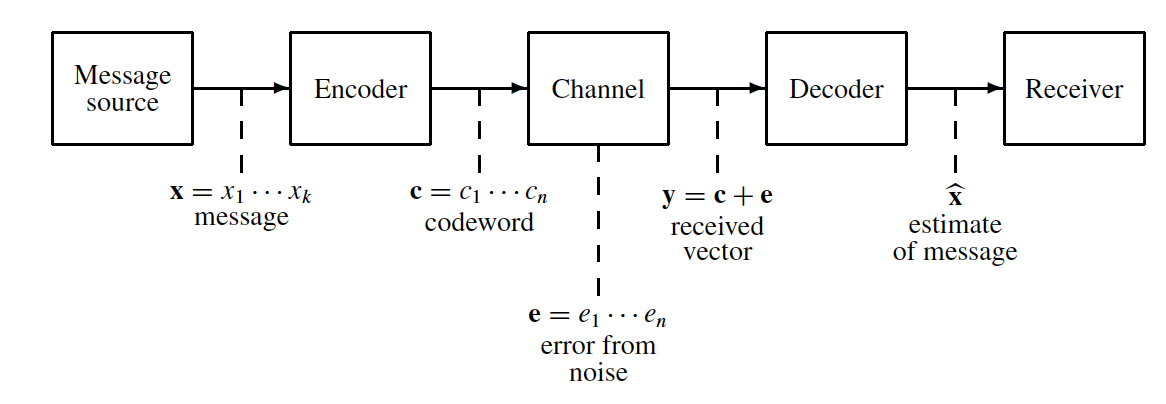
\includegraphics[width=0.7\textwidth]{./pic/LDPC-Codes1}}
        \caption{Kommunikationskanal}
        \label{fig:kommunikationskanal}
    \end{figure} 
    
    
    Die Kodierungstheorie beschäftigt sich damit, Informationen durch Ergänzung durch Redundanz so zu optimieren, dass sie den ursprünglichen Informationen gleichen. Dies geschieht indem der Kodierer die Information ergänzt, hier in der \autoref{fig:kommunikationskanal} als Codewort \(c\) benannt, und dann über einen Kanal übermittelt. Durch Rauschen, in der \autoref{fig:kommunikationskanal} als FehlerVektor \(e\) benannt, wird das Codewort verzerrt und man empfängt Vektor \(y\).
    
    
    Generell entspringen Codewort-Symbole aus einem Körper $\mathbb{F}_q$ mit \(q\) Elementen. Nachrichten und Codewörter sind Vektoren in den Vektorräumen $\mathbb{F}_{q}^{k}$ beziehungsweise $\mathbb{F}_{q}^{n}$.
    
    In \autoref{fig:kommunikationskanal} wird der FehlerVektor als \(e\) bezeichnet, dieser ist in der Abbildung die Differenz \( y - c \) aus dem Codewort \(c\), dass den Kanal betritt und dem empfangenden Vektor \(y\), der den Kanal verlässt. Die Abweichung zwischen dem Codewort \(c\)
    und dem Vektor \(y\) wird also durch den FehlerVektor \(e\) dargestellt. \cite[S. 2]{huffman}.
\end{Beispiel} 
    
    
    
\begin{definition}[Körper]
    Ein Körper ist eine algebraische Struktur. Diese besteht aus einer Menge und zwei Operationen die normalerweise als Mulitplikation mit $*$
    bezeichnet und als Addition mit $+$ bezeichnet benannt werden und bestimmte Axiome erfüllen. 
    Es gibt drei Körperer die man in der Untersuchung von linearen Codes sehr oft vorfindet. Diese sind das binäre Körper, mit zwei Elementen, das ternäre Körper mit drei Elementen und das quaternäre Körper mit vier Elementen. 
    
    \newpage
    Der Binärekörper $\mathbb{F}_2$ mit zwei Elementen \( \{0, 1\} \) hat die folgenden Additions- und Multiplikationstabellen
    
    \begin{table}[!h]
        \begin{center}
            \caption{Binärekörper $\mathbb{F}_2$}
            \label{tab:binäre Körper}
        \begin{tabular}{c|cc}
            
            $+$ & 0 & 1 \\
            \hline
            0 & 0 & 1 \\
            
            1 & 1 & 0 \\
            
            \end{tabular}
        \end{center}
        \end{table}
    
    \hfill
    
    \begin{table}[!h]
        \begin{center}
            \caption{Binärekörper $\mathbb{F}_2$}
            \label{tab:binäre Körper2}
            \begin{tabular}{c|cc}
                
                $*$& 0 & 1 \\
                \hline
                0 & 0 & 0 \\
                
                1 & 0 & 1 \\
                
                \end{tabular}
        \end{center}
        \end{table}
    \FloatBarrier
    Das ist auch der Ring der ganzen Zahlen Modulo 2. \\
    
    Der Ternärekörper $\mathbb{F}_3$ mit drei Elementen \( \{0, 1, 2\} \) hat Additions- und Multiplikationstabellen, die durch Addition und Multiplikation modulo 3 gegeben sind:
    
    
    \begin{table}[!h]
      \begin{center}
        \caption{Ternärekörper $\mathbb{F}_3$}
        \label{tab:ternäre Körper3}
        \begin{tabular}{c|ccc}
        
        $+$ & 0 & 1 & 2 \\
        \hline
        0 & 0 & 1 & 2 \\
        
        1 & 1 & 2 & 0 \\
        
        2 & 2 & 0 & 1 \\
        
        \end{tabular}
        \end{center}
    \end{table}
    
    \hfill
        \begin{table}[!h]
            \begin{center}
                \caption{Ternärekörper $\mathbb{F}_3$}
                \label{tab:ternäre Körper4}
                \begin{tabular}{c|ccc}
                
            $*$& 0 & 1 & 2 \\
            \hline
            0 & 0 & 0 & 0 \\
            
            1 & 0 & 1 & 2 \\
            
            2 & 0 & 2 & 1 \\
            
        \end{tabular}
    \end{center}
    \end{table}
    
    Der Quaternärekörper $\mathbb{F}_4$ mit vier Elementen \( \{0, 1, $\( \omega \)$, $\( \bar\omega\)$\} \) ist etwas komplizierter:\\ Er hat die folgenden Additions- und Multiplikationstabellen.\\
    $\mathbb{F}_4$ ist nicht der Ring der ganzen Zahlen, Modulo $4$:
    
    
    \begin{table}[!h]
        \begin{center}
          \caption{Quaternärekörper $\mathbb{F}_4$}
          \label{tab:quaternäre Körper5}
          \begin{tabular}{c|cccc}
            $+$ & 0 & 1 & $\omega$ & $\bar\omega$ \\
            \hline
            0 & 0 & 1 & $\omega$ & $\bar\omega$ \\
            1 & 1 & 0 & $\bar\omega$ & $\omega$ \\
            $\omega$ & $\omega$ & $\bar\omega$ & 0 & 1 \\
            $\bar\omega$ & $\bar\omega$ & $\omega$ & 1 & 0 \\
          \end{tabular}
          \end{center}
      \end{table}
    
    
    \hfill
    
        \begin{table}[!h]
        \begin{center}
            \caption{Quaternärekörper $\mathbb{F}_4$}
                \label{tab:quaternäre Körper6}
            \begin{tabular}{c|cccc}
            $*$ & 0 & 1 & $\omega$ & $\bar\omega$ \\
            \hline
            0 & 0 & 0 & 0 & 0 \\
            1 & 0 & 1 & $\omega$ & $\bar\omega$ \\
            $\omega$& 0 & $\omega$ & $\bar\omega$ & 1 \\
            $\bar\omega$& 0 & $\bar\omega$& 1 & $\omega$ \\
            \end{tabular}
            \end{center}
        \end{table}
    
       
    
    \FloatBarrier
    
    In diesen Tabellen sind einige grundlegende Gleichungen zu finden.\\
    Zum Beispiel stellt man fest, dass \( x + x = 0 \) für alle \(x\in\) $\mathbb{F}_4$ ist.\\ 
    Und $\bar\omega$ = $\omega^{2}$ = \( 1 + \omega \) und $\omega^{3}$ = $\bar\omega^{3} = 1$ sind.\cite[S. 3]{huffman} \\
\end{definition}

% ----------------------------
\section{Beispielmodell: Linearcodes, Generator- und Paritätsprüfmatrizen und Decodierung} 
% ----------------------------


\begin{definition}[Blockcodes]
    Ein \((n, k)\)-Blockcode \(C\) über dem Binärkörper \(\mathbb{F}_{2}\) ist eine Kodierung, bei der ein \(k\)-Bit langes Datenwort auf ein \(n\)-Bit langes Codewort abgebildet wird.
    
    Nachrichtenvektor mit den Datenbits:\\
    \(
    x = (x_1, \ldots, x_k) \in \mathbb{F}_{2}
    \).\\
    Es gibt \(2^k\) Nachrichtenvektoren der Datenlänge \(k\).\\
    
    Codewörter mit den Codebits:\\
    \(
    c = (c_1, \ldots, c_n) \in \mathbb{F}_{2}
    \).\\
    Es gibt \(2^k\) Nachrichtenvektoren der Datenlänge \(n\).\\
    
    Die Menge aller Codewörter ist definiert als:\\
    \(
    C = \{c \in \mathbb{F}_{2}^n\}
    \).\\

    Die Menge aller Nachrichtenvektoren ist definiert als:\\
    \(
    X = \{x \in \mathbb{F}_{2}^k\}
    \).\\

    Die Coderate \(h\) eines (\(n\),\(k\)) Codes, ist gegegben durch:\\
    \(
    k/n = h
    \).
\end{definition}
    
\begin{Beispiel}[Coderate]
    Der (\(5\),\(1\)) Blockcode besitzt eine Coderate \(h\) von:\\
    \(
    1/5 = 0,2
    \).
    Die Codewörter enthalten bei einer Kodierungsrate von $1/5$ nur $20\%$ Nutzdaten.\\
\end{Beispiel}
    
\begin{Beispiel}[Codewörter]
    Angenommen, es existiert ein (\(3\),\(2\)) Blockcode \(C\) über dem Binärkörper $\mathbb{F}_{2}$. Die Codewörter in \(C\) haben die Coderate $2/3$ und bestehen aus $2^2 = 4$ binären Vektoren der Codewortlänge $3$. Ein binärer Code kann durch eine Linearkombination der Basisvektoren dieses Untervektorraums dargestellt werden und beispielsweise folgende Form besitzen:
    
    $C = \{(c_1, c_2, c_3, c_4)\} = \{(1,1,0),(1,0,1),(0,1,1),(0,0,0)\}$
    \\
\end{Beispiel}
\pagebreak

\begin{Theorem}[linear Binärcode]
    Der (\(3\),\(2\)) Blockcode \(C\) hei\ss{}t dann linear, falls die Summe zweier Codewörter wieder ein Codewort ist:
\end{Theorem}
    
    
\begin{Beweis}
    $c_1, c_2, c_3, c_4 \in C \Rightarrow$ $(c_1 + c_i) \in C \quad (c_2 + c_{i}) \in C \quad (c_3 + c_{i}) \in C \quad (c_4 + c_{i}) \in C \quad mit\\ 
    \quad i \in \{1, 2, 3, 4\}$
    \\
    
    $(c_1 + c_1) = (1,1,0) + (1,1,0) = (2,2,0) \bmod 2 = (0,0,0) = c_4 \in C$
    
    $(c_2 + c_1) = (c_1 + c_2) = (1,1,0) + (1,0,1) = (2,1,1) \bmod 2 = (0,1,1) = c_3 \in C$
    
    $(c_3 + c_1) = (c_1 + c_3) = (1,1,0) + (0,1,1) = (1,2,1) \bmod 2 = (1,0,1) = c_2 \in C$
    
    $(c_4 + c_1) = (c_1 + c_4) = (1,1,0) + (0,0,0) = (1,1,0) = c_1 \in C$
    
    $(c_2 + c_2) = (1,0,1) + (1,0,1) = (2,0,2) \bmod 2 = (0,0,0) = c_4 \in C$
    
    $(c_3 + c_2) = (c_2 + c_3) = (1,0,1) + (0,1,1) = (1,1,2) \bmod 2 = (1,1,0) = c_1 \in C$
    
    $(c_4 + c_2) = (c_2 + c_4) = (1,0,1) + (0,0,0) = (1,0,1) = c_2 \in C$
    
    $(c_3 + c_3) = (0,1,1) + (0,1,1) = (0,2,2) \bmod 2 = (0,0,0) = c_4 \in C$
    
    $(c_4 + c_3) = (c_3 + c_4) = (0,1,1) + (0,0,0) = (0,1,1) = c_3 \in C$
    
    $(c_4 + c_4) = (c_4 + c_4) = (0,0,0) + (0,0,0) = (0,0,0) = c_4 \in C$. 
\end{Beweis}
    
\begin{Beispiel}
    Ein (\(3\),\(2\)) Blockcode \(C\) über dem Binärkörper $\mathbb{F}_{2}$, der die Bedingung der Linearität nicht erfüllt:
    
    $C = \{(c_1, c_2, c_3, c_4)\} = \{(1,1,0),(1,1,1),(0,1,1),(0,0,0)\}$\\
\end{Beispiel}
    
\begin{Beweis}
    $c_1, c_2, c_3, c_4 \in C \Rightarrow$ $(c_1 + c_i) \in C \quad (c_2 + c_{i}) \in C \quad (c_3 + c_{i}) \in C \quad (c_4 + c_{i}) \in C \quad mit\\
    \quad i \in \{1, 2, 3, 4\}$\\
    
    
    $(c_3 + c_1) = (c_1 + c_3) = (1,1,0) + (0,1,1) = (1,2,1) \bmod 2 = (1,0,1) \notin C.$\\ 
\end{Beweis}\cite{lntww2023} 
    
\begin{definition}[Generatormatrix und Paritätsprüfmatrix]
    Die Generatormatrix $G$ für den $[n,k]$ linearen Binärcode $C$ ist eine beliebige $k \times n$ Matrix, deren Zeilen eine Basis für $C$ bilden.
    Die Paritätsprüfungsmatrix $H$ für den $[n,k]$ linearen Binärcode $C$ ist eine beliebige $(n-k) \times n$ Matrix, deren Zeilen auch eine Basis für $C$ bilden. Sie beschreibt den $[n,k]$ linearen Binärcode $C$ durch Verwendung von korrigierter Fehlererkennung. Allgemein gibt es auch mehrere mögliche Paritätsprüfungsmatrizen $H$ für $C$.
    Wählt man sich beispielsweise eine Generatormatrix $G$ für den $[n,k]$ linearen Binärcode $C$, muss der folgende Ausdruck gelten: $HG^\intercal = 0$, damit die Zeilen von $H$ orthogonal zu allen Codewörtern sind. Ist dies nicht der Fall, würde $HG^\intercal \neq 0$ ergeben und die Paritätsprüfung würde eventuell ein fehlerhaftes Codewort prüfen. \cite[S. 4]{huffman}
\end{definition} 
    
    
    
\begin{Beispiel}[Generatormatrix und Paritätsprüfmatrix]
    F{\"u}r den $[3,2]$ linear Binärcode \(C\) ist $G$  eine $2 \times 3$ Matrix und $H$ eine $(3-2=1) \times 3$ Matrix:\\
    
    $G=\left( \begin{array}{rrr}
        1 & 1 & 0 \\
        0 & 1 & 1 \\
     \end{array}\right),
    $
    $G^\intercal=\left( \begin{array}{rrr}
    1 & 0 \\
    1 & 1 \\
    0 & 1 \\
    \end{array}\right), 
    $
    $H=\left( \begin{array}{rrr}
    x_1 & x_2 & x_3 \\
    \end{array}\right).
    $
    \\
    
    Lineares Gleichungssystem von $HG^\intercal = 0$ 
    
    $\left( \begin{array}{rrr}
    x_1+x_2 = 0 \\
    x_2+x_3 = 0 \\
    \end{array}\right).
    $
    
    Zieht man die Zeile zwei von der ersten ab erhält man:
    
    
    $x_1-x_3 = 0$.
    
    Wählt man nun $x_1 = 1$ ist auch $x_3 = 1$ durch Einsetzen in den einzelnen Zeilen $\Rightarrow$ $x_2 = 1$.
    d.h. 
    $H_1=\left( \begin{array}{rrr}
              1 & 1 & 1 \\
             \end{array}\right).
    $
    \\
    
    Wählt man nun $x_1 = 0$ ist auch $x_3 = 0$ durch Einsetzen in den einzelnen Zeilen $\Rightarrow$ $x_2 = 0$.
    d.h. 
    $H_2=\left( \begin{array}{rrr}
              0 & 0 & 0 \\
             \end{array}\right).
    $
    \\
    
    Lineares Gleichungssystem von $HG^\intercal = 1$ 
    
    $\left( \begin{array}{rrr}
    x_1+x_2 = 1 \\
    x_2+x_3 = 1 \\
    \end{array}\right).
    $
    
    Zieht man die Zeile zwei von der ersten ab erhält man:
    
    
    $x_1-x_3 = 0$.
    
    Wählt man nun $x_1 = 1$ ist auch $x_3 = 1$  durch Einsetzen in den einzelnen Zeilen $\Rightarrow$ $x_2 = 0$.
    d.h. 
    $H_3=\left( \begin{array}{rrr}
              1 & 0 & 1 \\
             \end{array}\right).
    $
    \\
    
    Wählt man nun $x_1 = 0$ ist auch $x_3 = 0$  durch Einsetzen in den einzelnen Zeilen $\Rightarrow$ $x_2 = 1$.
    d.h. 
    $H_4=\left( \begin{array}{rrr}
              0 & 1 & 0 \\
             \end{array}\right).
    $
    \\
    \end{Beispiel}
    
    \begin{Beispiel}[Generatormatrix und Paritätsprüfmatrix]
    F{\"u}r den $[4,2]$ Linearen Binärcode \(C\) ist $G$  eine $2 \times 4$ Matrix und $H$ eine $(4-2=2) \times 4$ Matrix:\\
    
    $G=\left( \begin{array}{rrrr}
        1 & 1 & 0 & 1\\
        0 & 1 & 1 & 1\\
     \end{array}\right),
    $
    $G^\intercal=\left( \begin{array}{rrr}
    1 & 0 \\
    1 & 1 \\
    0 & 1 \\
    1 & 1 \\
    \end{array}\right),
    $
    $H=\left( \begin{array}{rrrr}
    x_1 & x_2 & x_3 & x_4 \\
    x_1 & x_2 & x_3 & x_4 \\
    \end{array}\right).
    $
    \\
    
    Lineares Gleichungssystem von $HG^\intercal = 0$ 
    
    
    $\left( \begin{array}{rrr}
        x_1+x_2+x_4 = 0 & x_2+x_3+x_4 = 0 \\
        x_2+x_2+x_4 = 0 & x_2+x_3+x_4 = 0 \\
     \end{array}\right).
    $\\
    
    Zieht man die zweite Gleichung von der ersten ab, erhält man den Ausdruck:
    
    $x_1-x_3 = 0$.
    
    Wählt man nun $x_1=1$ ist auch $x_3=1$. 
    
    Durch Einsetzen in beide Gleichungen erhält man:
    
    $x_2+1+x_4=0$,
    $1+x_2+x_4=0$.
    
    Fall$1:$ $x_2=1$ dann muss $x_4=0$ sein. 
    
    Fall$2:$ $x_2=0$ dann muss $x_4=1$ sein.
    
    Hieraus ergeben sich zwei Möglichkeiten für $H$:
    
    
    $H_1=\left( \begin{array}{rrrr}
                 1 & 1 & 1 & 0 \\
                 1 & 0 & 1 & 1 \\
                \end{array}\right),
    $
    $H_2=\left( \begin{array}{rrrr}
        1 & 0 & 1 & 1 \\
        1 & 1 & 1 & 0 \\
       \end{array}\right).
    $\\
\pagebreak
    
    Wählt man nun $x_1=0$ ist auch $x_3=0$.
    
    Durch Einsetzen in beide Gleichungen erhält man:
    
    $x_2+x_4=0$,
    $x_2+x_4=0$.
    
    Fall$1:$ $x_2=1$ dann muss $x_4=1$ sein. 
    
    Fall$2:$ $x_2=0$ dann muss $x_4=0$ sein.
    
    Hieraus ergeben sich zwei Möglichkeiten für $H$:
    
    
    $H_3=\left( \begin{array}{rrrr}
        0 & 0 & 0 & 0 \\
        0 & 1 & 0 & 1 \\
       \end{array}\right),
    $
    $H_4=\left( \begin{array}{rrrr}
    0 & 1 & 0 & 1 \\
    0 & 0 & 0 & 0 \\
    \end{array}\right).
    $\\
\end{Beispiel}

    
\begin{Beispiel}[Codewörter, Nachrichtenvektoren, Generatormatrix und Paritätsprüfmatrix]
    Im Folgenden wird von einem
    $[3,2]$ linearen Binärcode \(C\) ausgegangen, der eine $2 \times 3$ Generatormatrix $G$ besitzt, zu dem es zwei $(3-2=1) \times 3$ Paitätsprüfmatrizen $H_1$ und $H_4$ gibt, wobei $H_1$ mit der Bedingung $HG^\intercal = 0$ erzeugt wurde und $H_4$ mit der Bedingung $HG^\intercal \neq 0$. 
    Der Vergleich und das Verhalten der beiden Paritätsprüfmatrizen wird anhand derselben Paritätsprüfung durchgeführt und dementsprechen erläutert.\\
    
    $G=\left( \begin{array}{rrr}
        1 & 1 & 0 \\
        0 & 1 & 1 \\
     \end{array}\right),
    $
    $G^\intercal=\left( \begin{array}{rrr}
    1 & 0 \\
    1 & 1 \\
    0 & 1 \\
    \end{array}\right), 
    $
    $H_1=\left( \begin{array}{rrr}
    1 & 1 & 1 \\
    \end{array}\right),
    $
    $H_4=\left( \begin{array}{rrr}
    0 & 1 & 0 \\
    \end{array}\right).
    $\\
    
    Jedes Codewort\\
    $c = (c_{1},c_{2},c_{3}) \in C$\\
    
    kann durch Multiplikation eines Nachrichtenvektoren\\
    $x = (x_{1},x_{2}) \in \mathbb{F}_{2}^{2}$\\
    
    mit der Generatormatrix \(G\) erhalten werden, d. h. es gilt:\\
    $c=xG = (x_1,x_1+x_2,x_2).$\\
    
    Der Binärvektor\\
    $c = (x_1,x_1+x_2,x_2) \in C$\\
    
    ist genau dann ein gültiges Codewort, wenn:
    
    $0 = H_1c^\intercal = (1,1,1) (x_1, x_1 + x_2, x_2)^\intercal = (2x_1+2x_2)$ gilt.\\
    $0 = H_4c^\intercal = (0,1,0) (x_1, x_1 + x_2, x_2)^\intercal = (x_1+x_2)$ gilt. \cite[S. 5]{huffman}\\
    
    
    Der Nachrichtenvektor $x = (x_{1},x_{2}) \in \mathbb{F}_{2}^{2}$  hat $2^2= 4$ Nachrichtenvektoren:
    
    
    $X = \{(x_1, x_2, x_3, x_4)\} = \{(0,0),(0,1),(1,0),(1,1)\}.$\\
    
    Durch Einsetzen der einzelnen Nachrichtenvektoren in $c = (x_1,x_1+x_2,x_2) \in C$\\ erhält man die einzelnen Binärvektoren:
    
    $x_1= (0,0)\Rightarrow c_1=(0,0+0,0)=(0,0,0)$
    
    $x_2= (0,1)\Rightarrow c_2=(0,0+1,1)=(0,1,1)$
    
    $x_3= (1,0)\Rightarrow c_3=(1,1+0,0)=(1,1,0)$
    
    $x_4= (1,1)\Rightarrow c_4=(1,1+1,1)=(1,2,1)\bmod 2=(1,0,1).$\\
    
    
    Dadurch sind unsere linearen Binärcodes definiert durch:
    
    $C = \{(c_1, c_2, c_3, c_4)\} = \{(0,0,0),(0,1,1),(1,1,0),(1,0,1)\}.$\\
    
    
    Um zu prüfen, ob es ein gültiges Codewort in $[3,2]$ linearen Binärcode \(C\) gibt prüft man für alle Codewörter ob:
    
    
    $0 = H_1c^\intercal = (2x_1+2x_2)$ und 
    $0 = H_4c^\intercal = (x_1+x_2)$
    
    für $H_1=\left( \begin{array}{rrr}
    1 & 1 & 1 \\
    \end{array}\right) 
    $ und
    $H_4=\left( \begin{array}{rrr}
    0 & 1 & 0 \\
    \end{array}\right)
    $ gilt.\\
    
    $H_1c^\intercal_1 =$$\left( \begin{array}{rrr}
    1 & 1 & 1 \\
    \end{array}\right) 
    $$(0,0,0)^\intercal=(2*0+2*0)=(0)$\\
    $H_1c^\intercal_2 =$$\left( \begin{array}{rrr}
    1 & 1 & 1 \\
    \end{array}\right) 
    $$(0,1,1)^\intercal=(2*0+2*1)=(2)\bmod 2= (0)$\\
    $H_1c^\intercal_3 =$$\left( \begin{array}{rrr}
    1 & 1 & 1 \\
    \end{array}\right) 
    $$(1,1,0)^\intercal=(2)\bmod 2=(0)=(2*1+2*1)=(4)\bmod 2= (0)$\\
    $H_1c^\intercal_4 =$$\left( \begin{array}{rrr}
    1 & 1 & 1 \\
    \end{array}\right) 
    $$(1,0,1)^\intercal=(2*1+2*0)=(2)\bmod 2= (0).$\\
    
    
    $H_4c^\intercal_1 =$$\left( \begin{array}{rrr}
    0 & 1 & 0 \\
    \end{array}\right) 
    $$(0,0,0)^\intercal=(0+0)=(0)$\\
    $H_4c^\intercal_2 =$$\left( \begin{array}{rrr}
    0 & 1 & 0 \\
    \end{array}\right) 
    $$(0,1,1)^\intercal=(0+1)=(1)$\\
    $H_4c^\intercal_3 =$$\left( \begin{array}{rrr}
    0 & 1 & 0 \\
    \end{array}\right) 
    $$(1,1,0)^\intercal=(1)\neq (1+1)=(2)\bmod 2= (0)$\\
    $H_4c^\intercal_4 =$$\left( \begin{array}{rrr}
    0 & 1 & 0 \\
    \end{array}\right) 
    $$(1,0,1)^\intercal=(0)\neq(1+0)=(1).$\\
    
    Alle Binärcodes $C=\{(c_1, c_2, c_3, c_4)\} = \{(0,0,0),(0,1,1),(1,1,0),(1,0,1)\}$ ergeben durch Einsetzen in $(0) = H_1c^\intercal$
    den Nullvektor und sind somit laut der Paritätspr{\"u}fungsmatrix $H_1$ gültige Codewörter. Trivialerweise gilt, dass auch für $H_2c^\intercal = (0,0,0)c^\intercal$. Durch die lineare Gleichung $HG^\intercal= 0$ wurde bereits dafür gesorgt, dass die Zeilen von $H_1$ orthogonal zu allen Codewörtern sind.\\
    
    Die Binärcodes $c_1 =(0,0,0)$ und $c_4=(1,0,1)$ ergeben durch $H_4c^\intercal = (0)$ den Nullvektor und sind somit laut der Paritätspr{\"u}fungsmatrix $H_4$ gültige Codewörter. 
    
    Die Binärcodes $c_2 =(0,1,1)$ und $c_3=(1,1,0)$ ergeben durch $H_4c^\intercal\neq(0)$ nicht den Nullvektor und sind somit laut der Paritätspr{\"u}fungsmatrix $H_4$ keine gültigen, sondern fehlerhafte Codewörter. Durch die Gleichung $HG^\intercal\neq0$  wurde bereits vermutet, dass die Zeilen von $H_4$ nicht orthogonal zu allen Codewörtern sind und die Paritätsprüfung somit fehlerhafte Codewörter prüft. Die fehlerhaften Codewörter können durch geeignete Dekodieralgorithmen korrigiert werden. 
\end{Beispiel}
    
\begin{definition}[Dekodierung]
    Die Dekodierung besteht darin, zu bestimmen, welcher Nachrichtenvektor 
    $x = (x_{1},x_{2}) \in \mathbb{F}_{2}^{2}$ gesendet wurde, wenn ein möglicherweise fehlerhaftes Codewort $r$ empfangen wird. Bei der Syndromdekodierung wird das Syndrom $s$ berechnet:\\
    $s = Hr^\intercal$.\\
    
    Wenn $s = 0$ ist, dann ist der Vektor $r$ im Code und wird als gültiges Codewort dekodiert, andernfalls ist $r$ fehlerhaft und kann beispielsweise durch eine Tabelle oder einen Dekodieralgorithmus korrigiert werden.\cite[S. 6]{huffman}
\end{definition}
    
    
\begin{Beispiel}[Dekodierung]
    $r = (1,1,1)$ und $e = (0,1,0)$ sind möglicherweise fehlerhaftes Vektoren zum Nachrichtenvektor 
    $x_4 = (1,1)$.
    
    Um das Syndrom $s$ zu bestimmen berechnet man folgendes für  $H_1=\left( \begin{array}{rrr}
        1 & 1 & 1 \\
       \end{array}\right) 
    $:
    
    $s = H_1r^\intercal = $$\left( \begin{array}{rrr}
        1 & 1 & 1 \\
       \end{array}\right) 
    $$(1,1,1)^\intercal = (3)\bmod 2= (1).$\\
    
    Somit ist $s = 1$ und der Vektor $r = (1,1,1)$ kein gültiges sondern ein fehlerhaftes Codewort.\\
    $s = H_1r^\intercal = $$\left( \begin{array}{rrr}
        1 & 1 & 1 \\
       \end{array}\right) 
    $$(0,1,0)^\intercal = (1).$\\
    
    Somit ist $s = 1$ und der Vektor $e = (0,1,0)$ kein gültiges sondern ein fehlerhaftes Codewort zum Nachrichtenvektor 
    $x_4 = (1,1)$. Dementsprechend werden $e = (0,1,0)$ und $r = (1,1,1)$ korrigiert und mit dem gültigem Codewort
    
    $c_4 =r+e=(1,1,1)+(0,1,0)=(1,2,1)\bmod 2 = (1,0,1)$ dekodiert.\\
\end{Beispiel}
\pagebreak

\begin{Beispiel}[Dekodierung]
        $r = (0,1,1)$ und $e = (0,0,1)$ sind möglicherweise fehlerhafte Vektoren zum Nachrichtenvektor 
        $x_4 = (0,1)$.
        
        Um das Syndrom $s$ zu bestimmen berechnet man folgendes für  $H_1=\left( \begin{array}{rrr}
            1 & 1 & 1 \\
           \end{array}\right) 
        $:
        
        $s = H_1r^\intercal = $$\left( \begin{array}{rrr}
            1 & 1 & 1 \\
           \end{array}\right) 
        $$(0,1,1)^\intercal = (2)\bmod 2= (0).$\\
        
        Somit ist $s = 0$ und der Vektor $r = (0,1,1)$ ein gültiges Codewort.\\
        $s = H_1r^\intercal = $$\left( \begin{array}{rrr}
            1 & 1 & 1 \\
           \end{array}\right) 
        $$(0,0,1)^\intercal = (1).$\\
        
        Somit ist $s = 1$ und der Vektor $e = (0,0,1)$ kein gültiges sondern ein fehlerhaftes Codewort zum Nachrichtenvektor 
        $x_4 = (0,1)$. Dementsprechend wird $e = (0,0,1)$ mit $r = (0,1,1)$ korrigiert und als gültiges Codewort dekodiert.\\
\end{Beispiel}
    
\begin{Beispiel}[Dekodierung]
        $r = (1,1,0)$ und $e = (1,0,0)$ sind möglicherweise fehlerhafte Vektoren zum Nachrichtenvektor 
    $x_4 = (0,1)$.
    
    Um das Syndrom $s$ zu bestimmen berechnet man folgendes für  $H_4=\left( \begin{array}{rrr}
        0 & 1 & 0 \\
       \end{array}\right) 
    $:
    
    $s = H_4r^\intercal = $$\left( \begin{array}{rrr}
        0 & 1 & 0 \\
       \end{array}\right) 
    $$(1,1,0)^\intercal = (1).$\\
    
    Somit ist $s = 1$ und der Vektor $r = (1,1,0)$ kein gültiges sondern ein fehlerhaftes Codewort.\\
    $s = H_4r^\intercal = $$\left( \begin{array}{rrr}
        0 & 1 & 0 \\
       \end{array}\right) 
    $$(1,0,0)^\intercal = (0).$\\
    
    Somit ist $s = 0$ und der Vektor $e = (1,0,0)$ kein gültiges sondern ein fehlerhaftes Codewort zum Nachrichtenvektor 
    $x_4 = (0,1)$. Dementsprechend wird $e = (1,0,0)$ mit $r = (1,1,0)$ korrigiert und als gültiges Codewort dekodiert.\\
    
\end{Beispiel}


\chapter{Definition von LDPC-Codes}
% ----------------------------
\begin{definition}[LDPC-Codes]
    Ein (\(n\),\(k\)) Blockcode \(C\) ist ein Low-Density-Parity-Check-Code, kurz (LDPC-Code), der durch eine $m \times n$ Paritätsprüfungsmatrix $H$ 
    spezifiziert ist, die überwiegend aus Nullen und nur aus einer geringen Anzahl von Einsen besteht. 
    Insbesondere ist ein (\(n\),\(c\),\(r\)) Low-Density-Code ein Code der Blocklänge $n$ mit einer $m \times n$ Paritätsprüfungsmatrix $H$,
    wie in \autoref{fig:Paritätsprüfungsmatrix (12×16) H F{\"u} einen (16, 3, 4) LDPC-Code}, 
    bei der jede Spalte eine kleine feste Anzahl $c$ von Einsen und jede Zeile eine kleine feste Anzahl $r$ von Einsen enthält.
    Die daraus resultierenden Codes werden auch als „reguläre“ LDPC-Codes bezeichnet.
    
    Zählt man die Anzahl der Einsen in $H$ nach Zeilen und Spalten, so ergibt sich die Beziehung $nc = mr$ zwischen den Parametern. Im Allgemeinen sollen $r$ und $c$ im Vergleich zu $n$ relativ klein sein, sodass die Dichte der Einsen in $H$ gering ist. Eine solche Matrix $H$ verringert deutlich den benötigten Rechenaufwand beim dekodieren.
    
    Eine natürliche Verallgemeinerung für LDPC-Codes besteht darin, dass die Zeilen- und Spaltengewichte von $H$ auf eine kontrollierte Weise variieren können, also wenn in den Reihen oder Spalten die Anzahl der Einsen nicht konstant ist. Die daraus resultierenden Codes werden auch als „irreguläre“ LDPC-Codes bezeichnet.
test
    
    \begin{figure}[!ht]
        \centering
         {\includegraphics[width=0.7\textwidth]{./pic/Paritätsprüfungsmatrix (12×16) H Für einen (16, 3, 4) LDPC-Code}}
          \caption{ Paritätspr{\"u}fungsmatrix \(12\times16\) H für einen (16, 3, 4) LDPC-Code}
        \label{fig:Paritätsprüfungsmatrix (12×16) H F{\"u} einen (16, 3, 4) LDPC-Code}
    \end{figure}
    
    
     Gallager entwickelte zwei iterative Dekodieralgorithmen zur Dekodierung von LDPC-Codes:\\
     der harte Entscheidungsdekodieralgorithmus und\\
     der weiche Entscheidungsdekodieralgorithmus.
    
     Zu dem harten Entscheidungsdekodieralgorithmus gibt es auch eine „sequentielle“ Version.
    \cite[S. 11]{huffman}
\end{definition}
\pagebreak
    
    
    % ----------------------------
    \section{Beispielmodell: Der harte Entscheidungsdekodierungsalgorithmus} 
    % ----------------------------
    
     
    \begin{Beispiel}[Der harte Entscheidungsdekodierungsalgorithmus]
    Angenommen, das Codewort $c$ wird mit einem (\(n\),\(c\),\(r\)) binären LDPC-Code $C$ übertragen und der Vektor $y$ wird empfangen.
    
    Bei der Berechnung des Syndroms $S=Hy^\intercal$ beeinflusst jedes empfangene Bit $y_i$ höchstens $c$ Komponenten dieses Syndroms, da das $i$-te Bit an $c$ Paritätsprüfungen teilnimmt.
    
    
    Wenn von allen Bits $S$, die an diesen $c$ Paritätsprüfungen beteiligt sind, nur das $i$-te Bit fehlerhaft ist, dann sind diese $c$ Komponenten von $Hy^\intercal=1$, was bedeutet, dass die Gleichungen der Paritätsprüfung nicht erfüllt sind. Dementsprechend können unter den Bits von $S$ noch andere Fehler existieren, was dazu führt, dass noch mehrere der $c$ Komponenten von $Hy^\intercal=1$ sind.
    \end{Beispiel}
    
    \begin{Theorem}[Der harte Entscheidungsdekodierungsalgorithmus]
    Der Algoritmus besteht im Prinzip aus vier Schritte:
    
    I. Berechnen Sie $Hy^\intercal$ und bestimmen Sie die unbefriedigten Paritätsprüfungen, d.h. die Paritätsprüfungen, bei denen die Zeilen von $Hy^\intercal=1$ gleich 1 sind mit.
    
    II. Berechnen Sie für jedes der $n$ Bits die Anzahl der unbefriedigten Paritätsprüfungen, die dieses Bit betreffen.
    
    III. Ändern Sie die Bits von $y$, die an der grö\ss{}ten Anzahl von unbefriedigenden Paritätsprüfungen beteiligt sind; nennen Sie den resultierenden Vektor erneut $y$. 
    
    IV. Iterativ I, II und III wiederholen, bis entweder $Hy^\intercal=0$ ist, 
    in welchem Fall der empfangene Vektor als dieses letzte $y$ dekodiert wird, oder bis eine bestimmte Anzahl von Iterationen erreicht ist, 
    in welchem Fall der empfangene Vektor nicht dekodiert wird.\\
    \end{Theorem}
    
    \begin{Beispiel}[Der harte Entscheidungsdekodierungsalgorithmus]
        Sei $C$ der (\(16\),\(3\),\(4\)) LDPC-Code mit einer $12 \times 16$ -Paritätsprüfungsmatrix $H$ aus 
        \autoref{fig:Paritätsprüfungsmatrix (12×16) H F{\"u} einen (16, 3, 4) LDPC-Code}.\\
        
        Angenommen:\\
        $y = (0,1,0,0,1,0,1,0,0,0,1,0,0,0,0,0)$ wird empfangen.\\
        
        Dann ist $Hy^\intercal = (1,2,1,0,1,1,2,0,1,2,0,1)^\intercal \bmod 2 = (1,0,1,0,1,1,0,0,1,0,0,1)^\intercal$.
        
        Es gibt sechs unbefriedigte Paritätsprüfungen in $Hy^\intercal$, dass hei\ss{}t, es gibt sechs Einsen in $Hy^\intercal.$\\
        Die Zeilen $H_1, H_3, H_5, H_6, H_9$ und $H_{12}$ von $H$ sind demnach daran beteiligt.\\ Dementsprechend werden die Bitstellen in diesen Zeilen untersucht und geprüft.\\
        
        $H_1= \left( \begin{array}{rrrrrrrrrrrrrrrr}
            1 & 1 & 1 & 1 & 0 & 0 & 0 & 0 & 0 & 0 & 0 & 0 & 0 & 0 & 0 & 0 \\
           \end{array}\right). 
        $\\
        Es treten vier Einsen an den Bitstellen $(1, 2, 3, 4)$ auf.\\
        
        $H_3= \left( \begin{array}{rrrrrrrrrrrrrrrr}
            0 & 0 & 0 & 0 & 0 & 0 & 0 & 0 & 1 & 1 & 1 & 1 & 0 & 0 & 0 & 0 \\
           \end{array}\right). 
        $\\
        Es treten vier Einsen an den Bitstellen $(9, 10, 11, 12)$ auf.\\
        
        $H_5= \left( \begin{array}{rrrrrrrrrrrrrrrr}
            1 & 0 & 0 & 0 & 1 & 0 & 0 & 0 & 1 & 0 & 0 & 0 & 1 & 0 & 0 & 0 \\
           \end{array}\right). 
        $\\
        Es treten vier Einsen an den Bitstellen $(1, 5, 9, 13)$ auf.\\
        
        $H_6= \left( \begin{array}{rrrrrrrrrrrrrrrr}
            0 & 1 & 0 & 0 & 0 & 1 & 0 & 0 & 0 & 1 & 0 & 0 & 0 & 1 & 0 & 0 \\
           \end{array}\right). 
        $\\
        Es treten vier Einsen an den Bitstellen $(2, 6, 10, 14)$ auf.\\
        
        $H_9= \left( \begin{array}{rrrrrrrrrrrrrrrr}
            1 & 0 & 0 & 0 & 0 & 1 & 0 & 0 & 0 & 0 & 1 & 0 & 0 & 0 & 0 & 1 \\
           \end{array}\right). 
        $\\
        Es treten vier Einsen an den Bitstellen $(1, 6, 11, 16)$ auf.\\
        
        $H_{12}= \left( \begin{array}{rrrrrrrrrrrrrrrr}
            0 & 0 & 0 & 1 & 1 & 0 & 0 & 0 & 0 & 1 & 0 & 0 & 0 & 0 & 1 & 0 \\
           \end{array}\right). 
        $\\
        Es treten vier Einsen an den Bitstellen $(4, 5, 10, 15)$ auf.\\
        
        
        
        
        Die Bitstellen $(1, 10)$ sind jeweils an drei und somit am meisten an unbefriedigten Paritätsprüfungen beteiligt.\\ 
        Bitstelle $1$ ist in den Zeilen $H_1$, $H_5$ und in $H_9$ mit einer Eins vertreten,\\
        während die Bitstelle $10$ in den Zeilen $H_3$, $H_6$ und in $H_{12}$ mit einer Eins besetzt ist.\\ 
        Alle anderen Bitstellen sind an höchstens zwei Paritätsprüfungen beteiligt.\\
        
         
        Ändert man also die Bitstellen $(1, 10)$ von $y$, erhält man ein neues
        
        $y_{1neu} = (1,1,0,0,1,0,1,0,0,1,1,0,0,0,0,0).$\\
        
        Durch Iteration stellt sich heraus:\\
        $Hy_{1neu}^\intercal=0.$\\
        
        Somit wird dieses letzte $y_{1neu}$ mit einem Abstand von zwei 
        zum empfangenen Vektor\\ 
        $y = (0,1,0,0,1,0,1,0,0,0,1,0,0,0,0,0)$ als gesendetes Codewort erklärt.\\ 
        
    \end{Beispiel}
    
    \begin{Beispiel}[Der harte Entscheidungsdekodierungsalgorithmus]
        Angenommen:\\
        $y = (1,1,0,0,1,0,1,0,0,0,0,0,0,0,0,0)$
        wird empfangen.\\
        
        Dann ist $Hy^\intercal = (2,2,0,0,2,1,1,0,1,2,0,1)^\intercal \bmod 2 =(0,0,0,0,0,1,1,0,1,0,0,1)^\intercal$.\\
        
        Es gibt vier unbefriedigte Paritätsprüfungen in $Hy^\intercal$, dass hei\ss{}t, es gibt vier Einsen in $Hy^\intercal.$\\
        Die Zeilen $H_6, H_7, H_9$ und $H_{12}$ von $H$ sind demnach daran beteiligt.\\ Dementsprechend werden die Bitstellen in diesen Zeilen untersucht und geprüft.\\
        
        
        $H_6= \left( \begin{array}{rrrrrrrrrrrrrrrr}
            0 & 1 & 0 & 0 & 0 & 1 & 0 & 0 & 0 & 1 & 0 & 0 & 0 & 1 & 0 & 0 \\
           \end{array}\right). 
        $\\
        Es treten vier Einsen an den Bitstellen $(2, 6, 10, 14)$ auf.\\
        
        $H_7= \left( \begin{array}{rrrrrrrrrrrrrrrr}
            0 & 0 & 1 & 0 & 0 & 0 & 1 & 0 & 0 & 0 & 1 & 0 & 0 & 0 & 1 & 0 \\
           \end{array}\right). 
        $\\
        Es treten vier Einsen an den Bitstellen $(3, 7, 11, 15)$ auf.\\
        
        $H_9= \left( \begin{array}{rrrrrrrrrrrrrrrr}
            1 & 0 & 0 & 0 & 0 & 1 & 0 & 0 & 0 & 0 & 1 & 0 & 0 & 0 & 0 & 1 \\
           \end{array}\right). 
        $\\
        Es treten vier Einsen an den Bitstellen $(1, 6, 11, 16)$ auf.\\
        
        $H_{12}= \left( \begin{array}{rrrrrrrrrrrrrrrr}
            0 & 0 & 0 & 1 & 1 & 0 & 0 & 0 & 0 & 1 & 0 & 0 & 0 & 0 & 1 & 0 \\
           \end{array}\right). 
        $\\
        Es treten vier Einsen an den Bitstellen $(4, 5, 10, 15)$ auf.\\
        
        
        Die Bitstellen $(6, 10, 11, 15)$ sind jeweils an zwei und somit am meisten an unbefriedigten Paritätsprüfungen beteiligt.\\ 
        Bitstelle $6$ ist in den Zeilen $H_6$ und $H_9$ mit einer Eins vertreten,\\
        Bitstelle $10$ ist in den Zeilen $H_6$ und $H_{12}$ mit einer Eins vertreten,\\
        Bitstelle $11$ ist in den Zeilen $H_7$ und $H_9$ mit einer Eins vertreten\\ 
        und Bitstelle $15$ ist in den Zeilen $H_7$ und $H_{12}$ mit einer Eins besetzt.\\
        \pagebreak
        
        Alle anderen Bitstellen sind an höchstens einer Paritätsprüfung beteiligt.\\
        Ändert man also die Bitstellen $(6, 10, 11, 15)$ von $y$, erhält man ein neues:\\
        $y_{1neu} = (1,1,0,0,1,1,1,0,0,1,1,0,0,0,1,0).$\\
        
        Durch Iteration stellt sich heraus:\\
        $Hy_{1neu}^\intercal = (2,3,2,1,2,3,3,0,3,2,0,3)^\intercal \bmod 2 =(0,1,0,1,0,1,1,0,1,0,0,1)^\intercal.$\\
        
        Es gibt sechs unbefriedigte Paritätsprüfungen in $Hy_{1neu}^\intercal$, dass hei\ss{}t, es gibt sechs Einsen in $Hy_{1neu}^\intercal.$\\
        Die Zeilen $H_2, H_4, H_6, H_7, H_9$ und $H_{12}$ von $H$ sind demnach daran beteiligt.\\ Dementsprechend werden die Bitstellen in diesen Zeilen untersucht und geprüft.\\
        
        $H_2= \left( \begin{array}{rrrrrrrrrrrrrrrr}
            0 & 0 & 0 & 0 & 1 & 1 & 1 & 1 & 0 & 0 & 0 & 0 & 0 & 0 & 0 & 0 \\
           \end{array}\right). 
        $\\
        Es treten vier Einsen an den Bitstellen $(5, 6, 7, 8)$ auf.\\
        
        $H_4= \left( \begin{array}{rrrrrrrrrrrrrrrr}
            0 & 0 & 0 & 0 & 0 & 0 & 0 & 0 & 0 & 0 & 0 & 0 & 1 & 1 & 1 & 1 \\
           \end{array}\right). 
        $\\
        Es treten vier Einsen an den Bitstellen $(13, 14, 15, 16)$ auf.\\
        
        $H_6= \left( \begin{array}{rrrrrrrrrrrrrrrr}
            0 & 1 & 0 & 0 & 0 & 1 & 0 & 0 & 0 & 1 & 0 & 0 & 0 & 1 & 0 & 0 \\
           \end{array}\right). 
        $\\
        Es treten vier Einsen an den Bitstellen $(2, 6, 10, 14)$ auf.\\
        
        $H_7= \left( \begin{array}{rrrrrrrrrrrrrrrr}
            0 & 0 & 1 & 0 & 0 & 0 & 1 & 0 & 0 & 0 & 1 & 0 & 0 & 0 & 1 & 0 \\
           \end{array}\right). 
        $\\
        Es treten vier Einsen an den Bitstellen $(3, 7, 11, 15)$ auf.\\
        
        $H_9= \left( \begin{array}{rrrrrrrrrrrrrrrr}
            1 & 0 & 0 & 0 & 0 & 1 & 0 & 0 & 0 & 0 & 1 & 0 & 0 & 0 & 0 & 1 \\
           \end{array}\right). 
        $\\
        Es treten vier Einsen an den Bitstellen $(1, 6, 11, 16)$ auf.\\
        
        $H_{12}= \left( \begin{array}{rrrrrrrrrrrrrrrr}
            0 & 0 & 0 & 1 & 1 & 0 & 0 & 0 & 0 & 1 & 0 & 0 & 0 & 0 & 1 & 0 \\
           \end{array}\right). 
        $\\
        Es treten vier Einsen an den Bitstellen $(4, 5, 10, 15)$ auf.\\
        
        Die Bitstellen $(6, 15)$ sind jeweils an drei und somit am meisten an unbefriedigten Paritätsprüfungen beteiligt.\\ 
        Bitstelle $6$ ist in den Zeilen $H_2$, $H_6$ und $H_9$ mit einer Eins vertreten,\\ 
        und Bitstelle $15$ ist in den Zeilen $H_4, H_7$ und $H_{12}$ mit einer Eins besetzt.\\
        Alle anderen Bitstellen sind an höchstens zwei Paritätsprüfungen beteiligt.\\
         
        Ändert man also die Bitstellen $(6, 15)$ von $y_{1neu}$, erhält man ein neues:\\
        $y_{2neu} = (1,1,0,0,1,0,1,0,0,1,1,0,0,0,0,0).$\\
        
        Durch Iteration stellt sich heraus:\\
        $Hy_{2neu}^\intercal=  (2,2,2,0,2,2,2,0,2,2,0,2)^\intercal \bmod 2= (0,0,0,0,0,0,0,0,0,0,0,0)^\intercal.$\\
         
        Somit wird dieses letzte $y_{2neu}$ mit einem Abstand von zwei 
        zum empfangenen Vektor\\
        $y = (1,1,0,0,1,0,1,0,0,0,0,0,0,0,0,0)$ als gesendetes Codewort erklärt.\\
        
    \end{Beispiel}
    
    \begin{Beispiel}[Der harte Entscheidungsdekodierungsalgorithmus]
        Angenommen:
    
        $y = (0,1,0,0,1,0,1,0,0,1,0,0,1,0,0,0)$ wird empfangen.\\
        
        Durch Iteration stellt sich heraus:\\
        $Hy^\intercal= (1,2,1,1,2,2,1,0,0,3,0,2)^\intercal \bmod 2= (1,0,1,1,0,0,1,0,0,1,0,0)^\intercal.$\\
        
        Es gibt fünf unbefriedigte Paritätsprüfungen in $Hy^\intercal$, dass hei\ss{}t, es gibt fünf Einsen in $Hy^\intercal.$\\
        Die Zeilen $H_1, H_3, H_4, H_7$ und $H_{10}$ von $H$ sind demnach daran beteiligt.\\ 
        Dementsprechend werden die Bitstellen in diesen Zeilen untersucht und geprüft.\\
        
        $H_1= \left( \begin{array}{rrrrrrrrrrrrrrrr}
            1 & 1 & 1 & 1 & 0 & 0 & 0 & 0 & 0 & 0 & 0 & 0 & 0 & 0 & 0 & 0 \\
           \end{array}\right). 
        $\\
        Es treten vier Einsen an den Bitstellen $(5, 6, 7, 8)$ auf.\\
        
        $H_3= \left( \begin{array}{rrrrrrrrrrrrrrrr}
            0 & 0 & 0 & 0 & 0 & 0 & 0 & 0 & 1 & 1 & 1 & 1 & 0 & 0 & 0 & 0 \\
           \end{array}\right). 
        $\\
        Es treten vier Einsen an den Bitstellen $(9, 10, 11, 12)$ auf.\\
        
        $H_4= \left( \begin{array}{rrrrrrrrrrrrrrrr}
            0 & 0 & 0 & 0 & 0 & 0 & 0 & 0 & 0 & 0 & 0 & 0 & 1 & 1 & 1 & 1 \\
           \end{array}\right). 
        $\\
        Es treten vier Einsen an den Bitstellen $(13, 14, 15, 16)$ auf.\\
        
        $H_7= \left( \begin{array}{rrrrrrrrrrrrrrrr}
            0 & 0 & 1 & 0 & 0 & 0 & 1 & 0 & 0 & 0 & 1 & 0 & 0 & 0 & 1 & 0 \\
           \end{array}\right). 
        $\\
        Es treten vier Einsen an den Bitstellen $(3, 7, 11, 15)$ auf.\\
        
        $H_{10}= \left( \begin{array}{rrrrrrrrrrrrrrrr}
            0 & 1 & 0 & 0 & 0 & 0 & 1 & 0 & 0 & 0 & 0 & 1 & 1 & 0 & 0 & 0 \\
           \end{array}\right). 
        $\\
        Es treten vier Einsen an den Bitstellen $(1, 6, 11, 16)$ auf.\\
        
        
        Die Bitstellen $(2, 3, 7, 11, 12, 13, 15)$ sind jeweils an zwei und somit am meisten an unbefriedigten Paritätsprüfungen beteiligt.\\ 
        Bitstelle $2$ ist in den Zeilen $H_1$ und $H_{10}$ mit einer Eins vertreten,\\ 
        Bitstelle $3$ ist in den Zeilen $H_1$ und $H_7$ mit einer Eins vertreten,\\
        Bitstelle $11$ ist in den Zeilen $H_3$ und $H_7$ mit einer Eins vertreten,\\
        Bitstelle $12$ ist in den Zeilen $H_3$ und $H_{10}$ mit einer Eins vertreten,\\
        Bitstelle $13$ ist in den Zeilen $H_4$ und $H_{10}$ mit einer Eins vertreten\\
        und Bitstelle $15$ ist in den Zeilen $H_4$ und $H_7$ mit einer Eins besetzt.\\
        Alle anderen Bitstellen sind an höchstens einer Paritätsprüfung beteiligt.\\
        
        Ändert man also die Bitstellen $(2, 3, 7, 11, 12, 13, 15)$ von $y$, erhält man ein neues:\\
        $y_{1neu} = (0,0,1,0,1,0,0,0,0,1,1,1,0,0,1,0).$\\
        
        Durch Iteration stellt sich heraus:\\
        $Hy_{1neu}^\intercal = (1,1,3,1,1,1,3,1,1,1,1,3)^\intercal \bmod 2 =(1,1,1,1,1,1,1,1,1,1,1,1)^\intercal.$\\
        
        Der All-Eins-Spaltenvektor bedeutet, dass alle Paritätsprüfungen in $Hy_{1neu}^\intercal$, unbefriedigt sind.\\ 
        Das hei\ss{}t, alle Zeilen in $Hy_{1neu}^\intercal$ bestehen aus Einsen.\\
        Alle Zeilen $H_1, H_2, H_3, H_4, H_5, H_6, H_7, H_8, H_9, H_{10}, H_{11}$ und $H_{12}$ von $H$ sind demnach daran beteiligt.\\
        Dementsprechend sind alle Bitstellen jeweils an drei und somit mit der maximalen Anzahl an unbefriedigten Paritätsprüfungen beteiligt.\\
        
        Demzufolge werden alle Bitstellen von $y_{1neu}$ geändert und man erhält ein neues:\\
        $y_{2neu} = (1,1,0,1,0,1,1,1,1,0,0,0,1,1,0,1).$\\
        
        Durch Iteration stellt sich heraus:\\
        $Hy_{2neu}^\intercal = (3,3,1,3,3,3,1,3,3,3,3,1)^\intercal \bmod 2 =(1,1,1,1,1,1,1,1,1,1,1,1)^\intercal.$\\
        
        Für diese Iteration ist $Hy_{2neu}^\intercal = (1,1,1,1,1,1,1,1,1,1,1,1)^\intercal$ 
        wieder der All-Eins-Spaltenvektor, was wiederum bedeutet, 
        dass alle Paritätsprüfungen in $Hy_{2neu}^\intercal$ unbefriedigt sind.
         
        Somit gilt für die nächste Iteration $y_{3neu} = y_{1neu} = (0,0,1,0,1,0,0,0,0,1,1,1,0,0,1,0).$\\ 
        und $Hy_{3neu}^\intercal = Hy_{1neu}^\intercal = (1,1,1,1,1,1,1,1,1,1,1,1)^\intercal$.\\ 
        Das hei\ss{}t, alle Bits werden wieder in $y_{1neu}$ zurückverwandelt.\\
        Die Iterationen sind eindeutig in einem Zyklus gefangen und werden niemals ein Codewort erreichen, 
        sodass der ursprünglich empfangene Vektor $y = (0,1,0,0,1,0,1,0,0,1,0,0,1,0,0,0)$ nicht entschlüsselbar ist.\\
        
    \end{Beispiel}
    
    \begin{Beispiel}[Der harte Entscheidungsdekodierungsalgorithmus]
        Angenommen:
    
        $y = (1,0,0,0,0,1,0,1,1,0,1,0,0,1,0,0)$ wird empfangen.\\
        
        Durch Iteration stellt sich heraus:\\
        $Hy^\intercal= (1,2,2,1,2,2,1,1,3,0,3,0)^\intercal \bmod 2= (1,0,0,1,0,0,1,1,1,0,1,0)^\intercal.$\\
        
        Es gibt sechs unbefriedigte Paritätsprüfungen in $Hy^\intercal$,
        dass hei\ss{}t, es gibt sechs Einsen in $Hy^\intercal.$\\
        Die Zeilen $H_1, H_4, H_7, H_8, H_9$ und $H_{11}$ von $H$ sind demnach daran beteiligt.\\ 
        Dementsprechend werden die Bitstellen in diesen Zeilen untersucht und geprüft.\\
        
        $H_1= \left( \begin{array}{rrrrrrrrrrrrrrrr}
            1 & 1 & 1 & 1 & 0 & 0 & 0 & 0 & 0 & 0 & 0 & 0 & 0 & 0 & 0 & 0 \\
           \end{array}\right). 
        $\\
        Es treten vier Einsen an den Bitstellen $(1, 2, 3, 4)$ auf.\\
        
        $H_4= \left( \begin{array}{rrrrrrrrrrrrrrrr}
            0 & 0 & 0 & 0 & 0 & 0 & 0 & 0 & 0 & 0 & 0 & 0 & 1 & 1 & 1 & 1 \\
           \end{array}\right). 
        $\\
        Es treten vier Einsen an den Bitstellen $(13, 14, 15, 16)$ auf.\\
        
        $H_7= \left( \begin{array}{rrrrrrrrrrrrrrrr}
            0 & 0 & 1 & 0 & 0 & 0 & 1 & 0 & 0 & 0 & 1 & 0 & 0 & 0 & 1 & 0 \\
           \end{array}\right). 
        $\\
        Es treten vier Einsen an den Bitstellen $(3, 7, 11, 15)$ auf.\\
        
        $H_8= \left( \begin{array}{rrrrrrrrrrrrrrrr}
            0 & 0 & 0 & 1 & 0 & 0 & 0 & 1 & 0 & 0 & 0 & 1 & 0 & 0 & 0 & 1 \\
           \end{array}\right). 
        $\\
        Es treten vier Einsen an den Bitstellen $(4, 8, 12, 16)$ auf.\\
        
        $H_9= \left( \begin{array}{rrrrrrrrrrrrrrrr}
            1 & 0 & 0 & 0 & 0 & 1 & 0 & 0 & 0 & 0 & 1 & 0 & 0 & 0 & 0 & 1 \\
           \end{array}\right). 
        $\\
        Es treten vier Einsen an den Bitstellen $(1, 6, 11, 16)$ auf.\\
        
        $H_{11}= \left( \begin{array}{rrrrrrrrrrrrrrrr}
            0 & 0 & 1 & 0 & 0 & 0 & 0 & 1 & 1 & 0 & 0 & 0 & 0 & 1 & 0 & 0 \\
           \end{array}\right). 
        $\\
        Es treten vier Einsen an den Bitstellen $(3, 8, 9, 14)$ auf.\\
        
        Die Bitstellen $(3, 16)$ sind jeweils an drei und somit am meisten an unbefriedigten Paritätsprüfungen beteiligt.\\ 
        Bitstelle $3$ ist in den Zeilen $H_1$ und $H_7$ und $H_{11}$ mit einer Eins vertreten\\
        und Bitstelle $16$ ist in den Zeilen $H_4$, $H_8$ und $H_9$ mit einer Eins besetzt.\\
        Alle anderen Bitstellen sind an höchstens zwei Paritätsprüfungen beteiligt.\\
         
        Ändert man also die Bitstellen $(3, 16)$ von $y$, erhält man ein neues:\\
        $y_{1neu} = (1,0,1,0,0,1,0,1,1,0,1,0,0,1,0,1).$\\
        
        Durch Iteration stellt sich heraus:\\
        $Hy_{1neu}^\intercal = (2,2,2,2,2,2,2,2,4,0,4,0)^\intercal \bmod 2 =(0,0,0,0,0,0,0,0,0,0,0,0)^\intercal.$\\
        
        Somit wird dieses letzte $y_{1neu}$ mit einem Abstand von zwei zum empfangenen Vektor\\
        $y = (1,0,0,0,0,1,0,1,1,0,1,0,0,1,0,0)$ als gesendetes Codewort erklärt.\\
        
    \end{Beispiel}
    \pagebreak
    
    
    \begin{Beispiel}[Der harte Entscheidungsdekodierungsalgorithmus]
        Angenommen:
    
        $y = (1,0,0,0,0,1,0,1,1,0,1,0,0,0,0,1)$ wird empfangen.\\
        
        Durch Iteration stellt sich heraus:\\
        $Hy^\intercal= (1,2,2,1,2,1,1,2,4,0,2,0)^\intercal \bmod 2= (1,0,0,1,0,1,1,0,0,0,0,0)^\intercal.$\\
        
        Es gibt vier unbefriedigte Paritätsprüfungen in $Hy^\intercal$,
        dass hei\ss{}t, es gibt vier Einsen in $Hy^\intercal.$\\
        Die Zeilen $H_1, H_4, H_6$ und $H_7$ von $H$ sind demnach daran beteiligt. 
        Dementsprechend werden die Bitstellen in diesen Zeilen untersucht und geprüft.\\
        
        
        $H_1= \left( \begin{array}{rrrrrrrrrrrrrrrr}
            1 & 1 & 1 & 1 & 0 & 0 & 0 & 0 & 0 & 0 & 0 & 0 & 0 & 0 & 0 & 0 \\
           \end{array}\right). 
        $\\
        Es treten vier Einsen an den Bitstellen $(1, 2, 3, 4)$ auf.\\
        
        $H_4= \left( \begin{array}{rrrrrrrrrrrrrrrr}
            0 & 0 & 0 & 0 & 0 & 0 & 0 & 0 & 0 & 0 & 0 & 0 & 1 & 1 & 1 & 1 \\
           \end{array}\right). 
        $\\
        Es treten vier Einsen an den Bitstellen $(13, 14, 15, 16)$ auf.\\
        
        $H_6= \left( \begin{array}{rrrrrrrrrrrrrrrr}
            0 & 1 & 0 & 0 & 0 & 1 & 0 & 0 & 0 & 1 & 0 & 0 & 0 & 1 & 0 & 0 \\
           \end{array}\right). 
        $\\
        Es treten vier Einsen an den Bitstellen $(2, 6, 10, 14)$ auf.\\
        
        $H_7= \left( \begin{array}{rrrrrrrrrrrrrrrr}
            0 & 0 & 1 & 0 & 0 & 0 & 1 & 0 & 0 & 0 & 1 & 0 & 0 & 0 & 1 & 0 \\
           \end{array}\right). 
        $\\
        Es treten vier Einsen an den Bitstellen $(3, 7, 11, 15)$ auf.\\
        
        
        
        Die Bitstellen $(2, 3, 14, 15)$ sind jeweils an zwei und somit am meisten an unbefriedigten Paritätsprüfungen beteiligt.\\ 
        Bitstelle $2$ ist in den Zeilen $H_1$ und $H_6$ mit einer Eins vertreten,\\ 
        Bitstelle $3$ ist in den Zeilen $H_1$ und $H_7$ mit einer Eins vertreten,\\
        Bitstelle $14$ ist in den Zeilen $H_4$ und $H_6$ mit einer Eins vertreten\\
        und Bitstelle $15$ ist in den Zeilen $H_4$ und $H_7$ mit einer Eins besetzt.\\
        Alle anderen Bitstellen sind an höchstens einer Paritätsprüfung beteiligt.\\
        
         
        Ändert man also die Bitstellen $(2, 3, 14, 15)$ von $y$, erhält man ein neues:\\
        $y_{1neu} = (1,1,1,0,0,1,0,1,1,0,1,0,0,1,1,1).$\\
        
        Durch Iteration stellt sich heraus:\\
        $Hy_{1neu}^\intercal = (3,2,2,3,2,3,3,2,4,1,4,1)^\intercal \bmod 2 =(1,0,0,1,0,1,1,0,0,1,0,1)^\intercal.$\\
        
        Es gibt sechs unbefriedigte Paritätsprüfungen in $Hy_{1neu}^\intercal$,
        dass hei\ss{}t, es gibt sechs Einsen in $Hy_{1neu}^\intercal.$\\
        Die Zeilen $H_1, H_4, H_6, H_7, H_{10}$ und $H_{12}$1 von $H$ sind demnach daran beteiligt.\\ 
        Dementsprechend werden die Bitstellen in diesen Zeilen untersucht und geprüft.\\
        
        $H_1= \left( \begin{array}{rrrrrrrrrrrrrrrr}
            1 & 1 & 1 & 1 & 0 & 0 & 0 & 0 & 0 & 0 & 0 & 0 & 0 & 0 & 0 & 0 \\
           \end{array}\right). 
        $\\
        Es treten vier Einsen an den Bitstellen $(1, 2, 3, 4)$ auf.\\
        
        $H_4= \left( \begin{array}{rrrrrrrrrrrrrrrr}
            0 & 0 & 0 & 0 & 0 & 0 & 0 & 0 & 0 & 0 & 0 & 0 & 1 & 1 & 1 & 1 \\
           \end{array}\right). 
        $\\
        Es treten vier Einsen an den Bitstellen $(13, 14, 15, 16)$ auf.\\
        
        
        $H_6= \left( \begin{array}{rrrrrrrrrrrrrrrr}
            0 & 1 & 0 & 0 & 0 & 1 & 0 & 0 & 0 & 1 & 0 & 0 & 0 & 1 & 0 & 0 \\
           \end{array}\right). 
        $\\
        Es treten vier Einsen an den Bitstellen $(2, 6, 10, 14)$ auf.\\
        
        $H_7= \left( \begin{array}{rrrrrrrrrrrrrrrr}
            0 & 0 & 1 & 0 & 0 & 0 & 1 & 0 & 0 & 0 & 1 & 0 & 0 & 0 & 1 & 0 \\
           \end{array}\right). 
        $\\
        Es treten vier Einsen an den Bitstellen $(3, 7, 11, 15)$ auf.\\
        
        $H_{10}= \left( \begin{array}{rrrrrrrrrrrrrrrr}
            0 & 1 & 0 & 0 & 0 & 0 & 1 & 0 & 0 & 0 & 0 & 1 & 1 & 0 & 0 & 0 \\
           \end{array}\right). 
        $\\
        Es treten vier Einsen an den Bitstellen $(2, 7, 12, 13)$ auf.\\
        
        $H_{12}= \left( \begin{array}{rrrrrrrrrrrrrrrr}
            0 & 0 & 0 & 1 & 1 & 0 & 0 & 0 & 0 & 1 & 0 & 0 & 0 & 0 & 1 & 0 \\
           \end{array}\right). 
        $\\
        Es treten vier Einsen an den Bitstellen $(4, 5, 10, 15)$ auf.\\
        
        
        Die Bitstellen $(2, 15)$ sind jeweils an drei und somit am meisten an unbefriedigten Paritätsprüfungen beteiligt.\\ 
        Bitstelle $2$ ist in den Zeilen $H_1$, $H_6$ und in $H_{10}$ mit einer Eins vertreten\\ 
        und Bitstelle $15$ ist in den Zeilen $H_4$, $H_7$ und in $H_{12}$ mit einer Eins besetzt.\\
        Alle anderen Bitstellen sind an höchstens zwei Paritätsprüfungen beteiligt.\\
         
        Ändert man also die Bitstellen $(2, 15)$ von $y_{1neu}$, erhält man ein neues:\\
        $y_{2neu} = (1,0,1,0,0,1,0,1,1,0,1,0,0,1,0,1).$\\
        
        Durch Iteration stellt sich heraus:\\
        $Hy_{2neu}^\intercal = (2,2,2,2,2,2,2,2,4,0,4,0)^\intercal \bmod 2 =(0,0,0,0,0,0,0,0,0,0,0,0)^\intercal.$\\
        
        Somit wird dieses letzte $y_{2neu}$ mit einem Abstand von zwei 
        zum empfangenen Vektor\\
        $y = (1,0,0,0,0,1,0,1,1,0,1,0,0,0,0,1)$ als gesendetes Codewort erklärt.\\ 
        
    \end{Beispiel}
    
    \begin{Beispiel}[Der harte Entscheidungsdekodierungsalgorithmus]
        Angenommen:
    
        $y = (0,1,1,0,1,1,0,1,1,0,1,0,0,1,0,1)$ wird empfangen.\\
        
        Durch Iteration stellt sich heraus:\\
        $Hy^\intercal= (2,3,2,2,2,3,2,2,3,1,4,1)^\intercal \bmod 2= (0,1,0,0,0,1,0,0,1,1,0,1)^\intercal.$\\
        
        Es gibt fünf unbefriedigte Paritätsprüfungen in $Hy^\intercal$,
        dass hei\ss{}t, es gibt fünf Einsen in $Hy^\intercal.$\\
        Die Zeilen $H_2, H_6, H_9, H_{10}$ und $H_{12}$ von $H$ sind demnach daran beteiligt.\\ 
        Dementsprechend werden die Bitstellen in diesen Zeilen untersucht und geprüft.\\
        
        $H_2= \left( \begin{array}{rrrrrrrrrrrrrrrr}
            0 & 0 & 0 & 0 & 1 & 1 & 1 & 1 & 0 & 0 & 0 & 0 & 0 & 0 & 0 & 0 \\
           \end{array}\right). 
        $\\
        Es treten vier Einsen an den Bitstellen $(5, 6, 7, 8)$ auf.\\
        
        $H_6= \left( \begin{array}{rrrrrrrrrrrrrrrr}
            0 & 1 & 0 & 0 & 0 & 1 & 0 & 0 & 0 & 1 & 0 & 0 & 0 & 1 & 0 & 0 \\
           \end{array}\right). 
        $\\
        Es treten vier Einsen an den Bitstellen $(2, 6, 10, 14)$ auf.\\
        
        $H_9= \left( \begin{array}{rrrrrrrrrrrrrrrr}
            1 & 0 & 0 & 0 & 0 & 1 & 0 & 0 & 0 & 0 & 1 & 0 & 0 & 0 & 0 & 1 \\
           \end{array}\right). 
        $\\
        Es treten vier Einsen an den Bitstellen $(1, 6, 11, 16)$ auf.\\
        
        $H_{10}= \left( \begin{array}{rrrrrrrrrrrrrrrr}
            0 & 1 & 0 & 0 & 0 & 0 & 1 & 0 & 0 & 0 & 0 & 1 & 1 & 0 & 0 & 0 \\
           \end{array}\right). 
        $\\
        Es treten vier Einsen an den Bitstellen $(1, 6, 11, 16)$ auf.\\
        
        $H_{12}= \left( \begin{array}{rrrrrrrrrrrrrrrr}
            0 & 0 & 0 & 1 & 1 & 0 & 0 & 0 & 0 & 1 & 0 & 0 & 0 & 0 & 1 & 0 \\
           \end{array}\right). 
        $\\
        Es treten vier Einsen an den Bitstellen $(4, 5, 10, 15)$ auf.\\
        
        Die Bitstelle $6$ ist jeweils an drei und somit am meisten an unbefriedigten Paritätsprüfungen beteiligt.\\ 
        Bitstelle $6$ ist in den Zeilen $H_2$, $H_6$ und in $H_9$ mit einer Eins vertreten\\ 
        Alle anderen Bitstellen sind an höchstens zwei Paritätsprüfungen beteiligt.\\
         
        Ändert man also die Bitstellen $6$ von $y$, erhält man ein neues:\\
        $y_{1neu} = (0,1,1,0,1,0,0,1,1,0,1,0,0,1,0,1).$\\
        
        
        Durch Iteration stellt sich heraus:\\
        $Hy_{1neu}^\intercal = (2,2,2,2,2,2,2,2,2,1,4,1)^\intercal \bmod 2 =(0,0,0,0,0,0,0,0,0,1,0,1)^\intercal.$\\
        
        Es gibt zwei unbefriedigte Paritätsprüfungen in $Hy^\intercal$,
        dass hei\ss{}t, es gibt zwei Einsen in $Hy^\intercal.$\\
        Die Zeilen $H_{10}$ und $H_{12}$ von $H$ sind demnach daran beteiligt.\\ 
        Dementsprechend werden die Bitstellen in diesen Zeilen untersucht und geprüft.\\
        
        $H_{10}= \left( \begin{array}{rrrrrrrrrrrrrrrr}
            0 & 1 & 0 & 0 & 0 & 0 & 1 & 0 & 0 & 0 & 0 & 1 & 1 & 0 & 0 & 0 \\
           \end{array}\right). 
        $\\
        Es treten vier Einsen an den Bitstellen $(1, 6, 11, 16)$ auf.\\
        
        $H_{12}= \left( \begin{array}{rrrrrrrrrrrrrrrr}
            0 & 0 & 0 & 1 & 1 & 0 & 0 & 0 & 0 & 1 & 0 & 0 & 0 & 0 & 1 & 0 \\
           \end{array}\right). 
        $\\
        Es treten vier Einsen an den Bitstellen $(4, 5, 10, 15)$ auf.\\
        
        
        Die Bitstellen $(2, 4, 5, 7, 10, 12, 13, 15)$ sind jeweils an einen und somit am meisten an unbefriedigten Paritätsprüfungen beteiligt.\\ 
        Bitstelle $2$ ist in der Zeile $H_{10}$ mit einer Eins vertreten,\\
        Bitstelle $4$ ist in der Zeile $H_{12}$ mit einer Eins vertreten,\\
        Bitstelle $5$ ist in der Zeile $H_{12}$ mit einer Eins vertreten,\\
        Bitstelle $7$ ist in der Zeile $H_{10}$ mit einer Eins vertreten,\\
        Bitstelle $10$ ist in der Zeile $H_{12}$ mit einer Eins vertreten,\\
        Bitstelle $12$ ist in der Zeile $H_{10}$ mit einer Eins vertreten,\\
        Bitstelle $13$ ist in der Zeile $H_{10}$ mit einer Eins vertreten\\      
        und Bitstelle $15$ ist in der Zeile $H_{12}$ mit einer Eins besetzt.\\
        Alle anderen Bitstellen sind an keiner Paritätsprüfung beteiligt.\\
        
        Ändert man also die Bitstellen $(2, 4, 5, 7, 10, 12, 13, 15)$  von $y_{1neu}$, erhält man ein neues:\\
        $y_{2neu} = (0,0,1,1,0,0,1,1,1,1,1,1,1,1,1,1).$\\
        
        Durch Iteration stellt sich heraus:\\
        $Hy_{2neu}^\intercal = (2,2,4,4,2,2,4,4,2,3,4,3)^\intercal \bmod 2 =(0,0,0,0,0,0,0,0,0,1,0,1)^\intercal.$\\
        
        Somit ist $Hy_{1neu}^\intercal = Hy_{2neu}^\intercal = (0,0,0,0,0,0,0,0,0,1,0,1)^\intercal.$\\
        Das wiederum hei\ss{}t, dass für den nächste Iterationschritt:\\
        $y_{3neu} = y_{1neu} = (0,1,1,0,1,0,0,1,1,0,1,0,0,1,0,1)$ gilt. Die Iterationen sind eindeutig in einem Zyklus gefangen, wobei abwechselnd 
        der Vektor $y_{1neu}$ und Vektor $y_{2neu}$ angezeigt werden und 
        das Syndrom $S= Hy^\intercal$ immer ungleich null ist.
        Daher wird $y_{2neu}$ niemals ein Codewort erreichen,
        sodass der ursprünglich empfangene Vektor $y = (0,1,1,0,1,1,0,1,1,0,1,0,0,1,0,1)$ nicht entschlüsselbar ist.\\
        \pagebreak
    \end{Beispiel}

    Im folgenden sei $H$ eine $15 \times 20$ Paritätspr{\"u}fungsmatrix die in  \autoref{fig:Paritätsprüfungsmatrix (15×20) H F{\"u} einen (20, 3, 4) LDPC-Code} dargestellt wird.
    
    \begin{figure}[!ht]
        \centering
         {\includegraphics[width=0.7\textwidth]{./pic/Paritätsprüfungsmatrix (15×20) H Für einen (20, 3, 4) LDPC-Code}}
        \caption{ Paritätspr{\"u}fungsmatrix  \(15\times20\) H für einen (20, 3, 4) LDPC-Code}
        \label{fig:Paritätsprüfungsmatrix (15×20) H F{\"u} einen (20, 3, 4) LDPC-Code}
    \end{figure} 
    

\begin{Beispiel}[Der harte Entscheidungsdekodierungsalgorithmus]
    Sei $C$ der (20, 3, 4) LDPC-Code mit einer $15 \times 20$ Paritätspr{\"u}fungsmatrix $H$\\
    Angenommen, dass
    
    $y = (1,0,0,0,1,0,0,0,0,0,0,0,0,1,0,0,0,1,0,0)$ wird empfangen.\\
    
    Durch Iteration stellt sich heraus:\\
    $Hy^\intercal= (1,1,0,1,1,2,0,2,0,0,2,0,0,1,1)^\intercal \bmod 2= (1,1,0,1,1,0,0,0,0,0,0,0,0,1,1)^\intercal.$\\
    
    
    Es gibt sechs unbefriedigte Paritätsprüfungen in $Hy^\intercal$,
    dass hei\ss{}t, es gibt sechs Einsen in $Hy^\intercal.$\\
    Die Zeilen $H_1, H_2, H_4, H_5, H_{14}$ und $H_{15}$ von $H$ sind demnach daran beteiligt.\\ 
    Dementsprechend werden die Bitstellen in diesen Zeilen untersucht und geprüft.\\
    
    $H_1= \left( \begin{array}{rrrrrrrrrrrrrrrrrrrr}
        1 & 1 & 1 & 1 & 0 & 0 & 0 & 0 & 0 & 0 & 0 & 0 & 0 & 0 & 0 & 0 & 0 & 0 & 0 & 0 \\
       \end{array}\right). 
    $\\
    Es treten vier Einsen an den Bitstellen $(1, 2, 3, 4)$ auf.\\
    
    $H_2= \left( \begin{array}{rrrrrrrrrrrrrrrrrrrr}
        0 & 0 & 0 & 0 & 1 & 1 & 1 & 1 & 0 & 0 & 0 & 0 & 0 & 0 & 0 & 0 & 0 & 0 & 0 & 0 \\
       \end{array}\right). 
    $\\
    Es treten vier Einsen an den Bitstellen $(5, 6, 7, 8)$ auf.\\
    
    $H_4= \left( \begin{array}{rrrrrrrrrrrrrrrrrrrr}
        0 & 0 & 0 & 0 & 0 & 0 & 0 & 0 & 0 & 0 & 0 & 0 & 1 & 1 & 1 & 1 & 0 & 0 & 0 & 0 \\
       \end{array}\right). 
    $\\
    Es treten vier Einsen an den Bitstellen $(13, 14, 15, 16)$ auf.\\
    
    $H_5= \left( \begin{array}{rrrrrrrrrrrrrrrrrrrr}
        0 & 0 & 0 & 0 & 0 & 0 & 0 & 0 & 0 & 0 & 0 & 0 & 0 & 0 & 0 & 0 & 1 & 1 & 1 & 1 \\
       \end{array}\right). 
    $\\
    Es treten vier Einsen an den Bitstellen $(17, 18, 19, 20)$ auf.\\
    
    $H_{14}=\left( \begin{array}{rrrrrrrrrrrrrrrrrrrr}
        0 & 0 & 0 & 1 & 0 & 0 & 0 & 0 & 1 & 0 & 0 & 0 & 0 & 1 & 0 & 0 & 1 & 0 & 0 & 0 \\
       \end{array}\right). 
    $\\
    Es treten vier Einsen an den Bitstellen $(4, 9, 14, 17)$ auf.\\
    
    $H_{15}=\left( \begin{array}{rrrrrrrrrrrrrrrrrrrr}
        0 & 0 & 0 & 0 & 1 & 0 & 0 & 0 & 0 & 1 & 0 & 0 & 0 & 0 & 1 & 0 & 0 & 0 & 0 & 1 \\
       \end{array}\right). 
    $\\
    Es treten vier Einsen an den Bitstellen $(5, 10, 15, 20)$ auf.\\
    \pagebreak
    
    
    Die Bitstellen $(1, 4, 5, 14, 15, 17, 20)$ sind jeweils an zwei und somit am meisten an unbefriedigten Paritätsprüfungen beteiligt.\\ 
    Bitstelle $4$ ist in den Zeilen $H_1$ und $H_{14}$ mit einer Eins vertreten,\\
    Bitstelle $5$ ist in den Zeilen $H_2$ und $H_{15}$  mit einer Eins vertreten,\\
    Bitstelle $14$ ist in den Zeilen $H_4$ und $H_{14}$  mit einer Eins vertreten,\\ 
    Bitstelle $15$ ist in den Zeilen $H_4$ und $H_{15}$ mit einer Eins vertreten,\\
    Bitstelle $17$ ist in den Zeilen $H_5$ und $H_{14}$ mit einer Eins vertreten\\    
    und Bitstelle $20$ ist in den Zeilen $H_5$ und $H_{15}$ mit einer Eins besetzt.\\
    Alle anderen Bitstellen sind an höchstens einer Paritätsprüfung beteiligt.\\
     
    Ändert man also die Bitstellen $(1, 4, 5, 14, 15, 17, 20)$ von $y$, erhält man ein neues:\\
    $y_{1neu} = (1,0,0,1,0,0,0,0,0,0,0,0,0,0,1,0,1,1,0,1).$\\
    
    Durch Iteration stellt sich heraus:\\
    $Hy_{1neu}^\intercal= (2,0,0,1,3,1,1,1,2,1,2,0,0,2,2)^\intercal \bmod 2= (0,0,0,1,1,1,1,1,0,1,0,0,0,0,0)^\intercal.$\\
    
    Es gibt sechs unbefriedigte Paritätsprüfungen in $Hy_{1neu}^\intercal$,
    dass hei\ss{}t, es gibt sechs Einsen in $Hy_{1neu}^\intercal.$\\
    Die Zeilen $H_4, H_5, H_6, H_7, H_8$ und $H_{10}$ von $H$ sind demnach daran beteiligt.\\ 
    Dementsprechend werden die Bitstellen in diesen Zeilen untersucht und geprüft.\\
    
    $H_4= \left( \begin{array}{rrrrrrrrrrrrrrrrrrrr}
        0 & 0 & 0 & 0 & 0 & 0 & 0 & 0 & 0 & 0 & 0 & 0 & 1 & 1 & 1 & 1 & 0 & 0 & 0 & 0 \\
       \end{array}\right). 
    $\\
    Es treten vier Einsen an den Bitstellen $(13, 14, 15, 16)$ auf.\\
    
    $H_5= \left( \begin{array}{rrrrrrrrrrrrrrrrrrrr}
        0 & 0 & 0 & 0 & 0 & 0 & 0 & 0 & 0 & 0 & 0 & 0 & 0 & 0 & 0 & 0 & 1 & 1 & 1 & 1 \\
       \end{array}\right). 
    $\\
    Es treten vier Einsen an den Bitstellen $(17, 18, 19, 20)$ auf.\\
    
    $H_6= \left( \begin{array}{rrrrrrrrrrrrrrrrrrrr}
        1 & 0 & 0 & 0 & 1 & 0 & 0 & 0 & 1 & 0 & 0 & 0 & 1 & 0 & 0 & 0 & 0 & 0 & 0 & 0 \\
       \end{array}\right). 
    $\\
    Es treten vier Einsen an den Bitstellen $(1, 5, 9, 13)$ auf.\\
    
    $H_7= \left( \begin{array}{rrrrrrrrrrrrrrrrrrrr}
        0 & 1 & 0 & 0 & 0 & 1 & 0 & 0 & 0 & 1 & 0 & 0 & 0 & 0 & 0 & 0 & 1 & 0 & 0 & 0 \\
       \end{array}\right). 
    $\\
    Es treten vier Einsen an den Bitstellen $(2, 6, 10, 17)$ auf.\\
    
    $H_8=\left( \begin{array}{rrrrrrrrrrrrrrrrrrrr}
        0 & 0 & 1 & 0 & 0 & 0 & 1 & 0 & 0 & 0 & 0 & 0 & 0 & 1 & 0 & 0 & 0 & 1 & 0 & 0 \\
       \end{array}\right). 
    $\\
    Es treten vier Einsen an den Bitstellen $(3, 7, 14, 18)$ auf.\\
    
    $H_{10}=\left( \begin{array}{rrrrrrrrrrrrrrrrrrrr}
        0 & 0 & 0 & 0 & 0 & 0 & 0 & 0 & 1 & 0 & 0 & 0 & 1 & 0 & 0 & 1 & 0 & 0 & 0 & 1 \\
       \end{array}\right). 
    $\\
    Es treten vier Einsen an den Bitstellen $(8, 12, 16, 20)$ auf.\\
    
    
    Die Bitstellen $(13, 14, 16, 17, 18, 20)$ sind jeweils an zwei und somit am meisten an unbefriedigten Paritätsprüfungen beteiligt.\\ 
    Bitstelle $13$ ist in den Zeilen $H_4$ und $H_6$ mit einer Eins vertreten,\\
    Bitstelle $14$ ist in den Zeilen $H_4$ und $H_8$  mit einer Eins vertreten,\\
    Bitstelle $16$ ist in den Zeilen $H_4$ und $H_{10}$  mit einer Eins vertreten,\\ 
    Bitstelle $17$ ist in den Zeilen $H_5$ und $H_7$ mit einer Eins vertreten,\\
    Bitstelle $18$ ist in den Zeilen $H_5$ und $H_8$ mit einer Eins vertreten\\    
    und Bitstelle $20$ ist in den Zeilen $H_5$ und $H_{10}$ mit einer Eins besetzt.\\
    \pagebreak
    
    Alle anderen Bitstellen sind an höchstens einer Paritätsprüfung beteiligt.\\
    Ändert man also die Bitstellen $(13, 14, 16, 17, 18, 20)$ von $y_{1neu}$, erhält man ein neues:\\
    $y_{2neu} = (1,0,0,1,0,0,0,0,0,0,0,0,1,1,1,1,0,0,0,0).$\\
    
    Durch Iteration stellt sich heraus:\\
    $Hy_{2neu}^\intercal= (2,0,0,4,0,2,0,1,2,1,1,1,1,2,1)^\intercal \bmod 2= (0,0,0,0,0,0,0,1,0,1,1,1,1,0,1)^\intercal.$\\
    
    Es gibt sechs unbefriedigte Paritätsprüfungen in $Hy_{2neu}^\intercal$,
    dass hei\ss{}t, es gibt sechs Einsen in $Hy_{2neu}^\intercal.$\\
    Die Zeilen $H_8, H_{10}, H_{11}, H_{12}, H_{13}$ und $H_{15}$ von $H$ sind demnach daran beteiligt.\\ 
    Dementsprechend werden die Bitstellen in diesen Zeilen untersucht und geprüft.\\
    
    $H_8=\left( \begin{array}{rrrrrrrrrrrrrrrrrrrr}
        0 & 0 & 1 & 0 & 0 & 0 & 1 & 0 & 0 & 0 & 0 & 0 & 0 & 1 & 0 & 0 & 0 & 1 & 0 & 0 \\
       \end{array}\right). 
    $\\
    Es treten vier Einsen an den Bitstellen $(3, 7, 14, 18)$ auf.\\
    
    $H_{10}=\left( \begin{array}{rrrrrrrrrrrrrrrrrrrr}
        0 & 0 & 0 & 0 & 0 & 0 & 0 & 0 & 1 & 0 & 0 & 0 & 1 & 0 & 0 & 1 & 0 & 0 & 0 & 1 \\
       \end{array}\right). 
    $\\
    Es treten vier Einsen an den Bitstellen $(8, 12, 16, 20)$ auf.\\
    
    $H_{11}= \left( \begin{array}{rrrrrrrrrrrrrrrrrrrr}
        1 & 0 & 0 & 0 & 0 & 1 & 0 & 0 & 0 & 0 & 0 & 1 & 0 & 0 & 0 & 0 & 0 & 1 & 0 & 0 \\
       \end{array}\right). 
    $\\
    Es treten vier Einsen an den Bitstellen $(1, 6, 12, 18)$ auf.\\
    
    $H_{12}= \left( \begin{array}{rrrrrrrrrrrrrrrrrrrr}
        0 & 1 & 0 & 0 & 0 & 0 & 1 & 0 & 0 & 0 & 1 & 0 & 0 & 0 & 0 & 1 & 0 & 0 & 0 & 0 \\
       \end{array}\right). 
    $\\
    Es treten vier Einsen an den Bitstellen $(2, 7, 11, 16)$ auf.\\
    
    $H_{13}= \left( \begin{array}{rrrrrrrrrrrrrrrrrrrr}
        0 & 0 & 1 & 0 & 0 & 0 & 0 & 1 & 0 & 0 & 0 & 0 & 1 & 0 & 0 & 0 & 0 & 0 & 1 & 0 \\
       \end{array}\right). 
    $\\
    Es treten vier Einsen an den Bitstellen $(3, 8, 13, 19)$ auf.\\
    
    $H_{15}=\left( \begin{array}{rrrrrrrrrrrrrrrrrrrr}
        0 & 0 & 0 & 0 & 1 & 0 & 0 & 0 & 0 & 1 & 0 & 0 & 0 & 0 & 1 & 0 & 0 & 0 & 0 & 1 \\
       \end{array}\right). 
    $\\
    Es treten vier Einsen an den Bitstellen $(5, 10, 15, 20)$ auf.\\
    
    Die Bitstellen $(3, 7, 8, 12, 16, 18, 20)$ sind jeweils an zwei und somit am meisten an unbefriedigten Paritätsprüfungen beteiligt.\\ 
    Bitstelle $3$ ist in den Zeilen $H_8$ und $H_{13}$ mit einer Eins vertreten,\\
    Bitstelle $7$ ist in den Zeilen $H_8$ und $H_{12}$  mit einer Eins vertreten,\\
    Bitstelle $8$ ist in den Zeilen $H_{10}$ und $H_{13}$  mit einer Eins vertreten,\\ 
    Bitstelle $12$ ist in den Zeilen $H_{10}$ und $H_{11}$ mit einer Eins vertreten,\\
    Bitstelle $16$ ist in den Zeilen $H_{10}$ und $H_{12}$ mit einer Eins vertreten\\   
    Bitstelle $18$ ist in den Zeilen $H_8$ und $H_{11}$ mit einer Eins vertreten\\   
    und Bitstelle $20$ ist in den Zeilen $H_{10}$ und $H_{15}$ mit einer Eins besetzt.\\
    Alle anderen Bitstellen sind an höchstens einer Paritätsprüfung beteiligt.\\
    
    Ändert man also die Bitstellen $(3, 7, 8, 12, 16, 18, 20)$ von $y_{2neu}$, erhält man ein neues:\\
    $y_{3neu} = (1,0,1,1,0,0,1,1,0,0,0,1,1,1,1,0,0,1,0,1).$\\
    
    Durch Iteration stellt sich heraus:\\
    $Hy_{3neu}^\intercal= (3,2,1,3,2,2,0,4,2,3,3,1,3,2,2)^\intercal \bmod 2= (1,0,1,1,0,0,0,0,0,1,1,1,1,0,0)^\intercal.$\\
    
    Es gibt sieben unbefriedigte Paritätsprüfungen in $Hy_{3neu}^\intercal$,
    dass hei\ss{}t, es gibt sieben Einsen in $Hy_{3neu}^\intercal.$\\
    Die Zeilen $H_1, H_3, H_4, H_{10}, H_{11}, H_{12} $ und $H_{13}$ von $H$ sind demnach daran beteiligt.\\ 
    Dementsprechend werden die Bitstellen in diesen Zeilen untersucht und geprüft.\\
    \pagebreak
    
    $H_1= \left( \begin{array}{rrrrrrrrrrrrrrrrrrrr}
        1 & 1 & 1 & 1 & 0 & 0 & 0 & 0 & 0 & 0 & 0 & 0 & 0 & 0 & 0 & 0 & 0 & 0 & 0 & 0 \\
       \end{array}\right). 
    $\\
    Es treten vier Einsen an den Bitstellen $(1, 2, 3, 4)$ auf.\\
    
    $H_3= \left( \begin{array}{rrrrrrrrrrrrrrrrrrrr}
        0 & 0 & 0 & 0 & 0 & 0 & 0 & 0 & 1 & 1 & 1 & 1 & 0 & 0 & 0 & 0 & 0 & 0 & 0 & 0 \\
       \end{array}\right). 
    $\\
    Es treten vier Einsen an den Bitstellen $(9, 10, 11, 12)$ auf.\\
    
    $H_4= \left( \begin{array}{rrrrrrrrrrrrrrrrrrrr}
        0 & 0 & 0 & 0 & 0 & 0 & 0 & 0 & 0 & 0 & 0 & 0 & 1 & 1 & 1 & 1 & 0 & 0 & 0 & 0 \\
       \end{array}\right). 
    $\\
    Es treten vier Einsen an den Bitstellen $(13, 14, 15, 16)$ auf.\\
    
    $H_{10}=\left( \begin{array}{rrrrrrrrrrrrrrrrrrrr}
        0 & 0 & 0 & 0 & 0 & 0 & 0 & 0 & 1 & 0 & 0 & 0 & 1 & 0 & 0 & 1 & 0 & 0 & 0 & 1 \\
       \end{array}\right). 
    $\\
    Es treten vier Einsen an den Bitstellen $(8, 12, 16, 20)$ auf.\\
    
    $H_{11}= \left( \begin{array}{rrrrrrrrrrrrrrrrrrrr}
        1 & 0 & 0 & 0 & 0 & 1 & 0 & 0 & 0 & 0 & 0 & 1 & 0 & 0 & 0 & 0 & 0 & 1 & 0 & 0 \\
       \end{array}\right). 
    $\\
    Es treten vier Einsen an den Bitstellen $(1, 6, 12, 18)$ auf.\\
    
    $H_{12}= \left( \begin{array}{rrrrrrrrrrrrrrrrrrrr}
        0 & 1 & 0 & 0 & 0 & 0 & 1 & 0 & 0 & 0 & 1 & 0 & 0 & 0 & 0 & 1 & 0 & 0 & 0 & 0 \\
       \end{array}\right). 
    $\\
    Es treten vier Einsen an den Bitstellen $(2, 7, 11, 16)$ auf.\\
    
    $H_{13}= \left( \begin{array}{rrrrrrrrrrrrrrrrrrrr}
        0 & 0 & 1 & 0 & 0 & 0 & 0 & 1 & 0 & 0 & 0 & 0 & 1 & 0 & 0 & 0 & 0 & 0 & 1 & 0 \\
       \end{array}\right). 
    $\\
    Es treten vier Einsen an den Bitstellen $(3, 8, 13, 19)$ auf.\\
    
    Die Bitstellen $(12, 16)$ sind jeweils an drei und somit am meisten an unbefriedigten Paritätsprüfungen beteiligt.\\ 
    Bitstelle $12$ ist in den Zeilen $H_3$, $H_{10}$ und $H_{11}$ mit einer Eins vertreten\\
    und Bitstelle $16$ ist in den Zeilen $H_4$, $H_{10}$ und $H_{12}$ mit einer Eins besetzt.\\
    Alle anderen Bitstellen sind an höchstens zwei Paritätsprüfungen beteiligt.\\
     
    Ändert man also die Bitstellen $(12, 16)$ von $y_{3neu}$, erhält man ein neues:\\
    $y_{4neu} = (1,0,1,1,0,0,1,1,0,0,0,0,1,1,1,1,0,1,0,1).$\\
    
    Durch Iteration stellt sich heraus:\\
    $Hy_{4neu}^\intercal= (3,2,0,4,2,2,0,4,2,3,2,2,3,2,2)^\intercal \bmod 2= (1,0,0,0,0,0,0,0,0,1,0,0,1,0,0)^\intercal.$\\
    
    Es gibt drei unbefriedigte Paritätsprüfungen in $Hy_{4neu}^\intercal$,
    dass hei\ss{}t, es gibt drei Einsen in $Hy_{4neu}^\intercal.$\\
    Die Zeilen $H_1, H_{10}$ und $H_{13}$ von $H$ sind demnach daran beteiligt.\\ 
    Dementsprechend werden die Bitstellen in diesen Zeilen untersucht und geprüft.\\
    
    $H_1= \left( \begin{array}{rrrrrrrrrrrrrrrrrrrr}
        1 & 1 & 1 & 1 & 0 & 0 & 0 & 0 & 0 & 0 & 0 & 0 & 0 & 0 & 0 & 0 & 0 & 0 & 0 & 0 \\
       \end{array}\right). 
    $\\
    Es treten vier Einsen an den Bitstellen $(1, 2, 3, 4)$ auf.\\
    
    $H_{10}=\left( \begin{array}{rrrrrrrrrrrrrrrrrrrr}
        0 & 0 & 0 & 0 & 0 & 0 & 0 & 0 & 1 & 0 & 0 & 0 & 1 & 0 & 0 & 1 & 0 & 0 & 0 & 1 \\
       \end{array}\right). 
    $\\
    Es treten vier Einsen an den Bitstellen $(8, 12, 16, 20)$ auf.\\
    
    $H_{13}= \left( \begin{array}{rrrrrrrrrrrrrrrrrrrr}
        0 & 0 & 1 & 0 & 0 & 0 & 0 & 1 & 0 & 0 & 0 & 0 & 1 & 0 & 0 & 0 & 0 & 0 & 1 & 0 \\
       \end{array}\right). 
    $\\
    Es treten vier Einsen an den Bitstellen $(3, 8, 13, 19)$ auf.\\
    
    Die Bitstellen $(3, 8)$ sind jeweils an zwei und somit am meisten an unbefriedigten Paritätsprüfungen beteiligt.\\
    Bitstelle $3$ ist in den Zeilen $H_1$ und $H_{13}$ mit einer Eins vertreten\\
    und Bitstelle $8$ ist in den Zeilen $H_{10}$ und $H_{13}$ mit einer Eins besetzt.\\
    \pagebreak
    
    Alle anderen Bitstellen sind an höchstens einer Paritätsprüfung beteiligt.\\
    Ändert man also die Bitstellen $(3, 8)$ von $y_{4neu}$, erhält man ein neues:\\
    $y_{5neu} = (1,0,0,1,0,0,1,0,0,0,0,0,1,1,1,1,0,1,0,1).$\\
    
    Durch Iteration stellt sich heraus:\\
    $Hy_{5neu}^\intercal= (2,1,0,4,2,2,0,3,2,2,2,2,1,2,2)^\intercal \bmod 2= (0,1,0,0,0,0,0,1,0,0,0,0,1,0,0)^\intercal.$\\
    
    Es gibt drei unbefriedigte Paritätsprüfungen in $Hy_{5neu}^\intercal$,
    dass hei\ss{}t, es gibt drei Einsen in $Hy_{5neu}^\intercal.$\\
    Die Zeilen $H_2, H_8$ und $H_{13}$ von $H$ sind demnach daran beteiligt.\\ 
    Dementsprechend werden die Bitstellen in diesen Zeilen untersucht und geprüft.\\
    
    $H_2= \left( \begin{array}{rrrrrrrrrrrrrrrrrrrr}
        0 & 0 & 0 & 0 & 1 & 1 & 1 & 1 & 0 & 0 & 0 & 0 & 0 & 0 & 0 & 0 & 0 & 0 & 0 & 0 \\
       \end{array}\right). 
    $\\
    Es treten vier Einsen an den Bitstellen $(5, 6, 7, 8)$ auf.\\
    
    $H_8=\left( \begin{array}{rrrrrrrrrrrrrrrrrrrr}
        0 & 0 & 1 & 0 & 0 & 0 & 1 & 0 & 0 & 0 & 0 & 0 & 0 & 1 & 0 & 0 & 0 & 1 & 0 & 0 \\
       \end{array}\right). 
    $\\
    Es treten vier Einsen an den Bitstellen $(3, 7, 14, 18)$ auf.\\
    
    $H_{13}= \left( \begin{array}{rrrrrrrrrrrrrrrrrrrr}
        0 & 0 & 1 & 0 & 0 & 0 & 0 & 1 & 0 & 0 & 0 & 0 & 1 & 0 & 0 & 0 & 0 & 0 & 1 & 0 \\
       \end{array}\right). 
    $\\
    Es treten vier Einsen an den Bitstellen $(3, 8, 13, 19)$ auf.\\
    
    Die Bitstellen $(3, 7, 8)$ sind jeweils an zwei und somit am meisten an unbefriedigten Paritätsprüfungen beteiligt.\\
    Bitstelle $3$ ist in den Zeilen $H_8$ und $H_{13}$ mit einer Eins vertreten,\\
    Bitstelle $7$ ist in den Zeilen $H_2$ und $H_8$ mit einer Eins vertreten\\
    und Bitstelle $8$ ist in den Zeilen $H_2$ und $H_{13}$ mit einer Eins besetzt.\\
    Alle anderen Bitstellen sind an höchstens einer Paritätsprüfung beteiligt.\\
    
    Ändert man also die Bitstellen $(3, 7, 8)$ von $y_{5neu}$, erhält man ein neues:\\
    $y_{6neu} = (1,0,1,1,0,0,0,1,0,0,0,0,1,1,1,1,0,1,0,1).$\\
    
    Durch Iteration stellt sich heraus:\\
    $Hy_{6neu}^\intercal= (3,1,0,4,2,2,0,3,2,3,2,1,3,2,2)^\intercal \bmod 2= (1,1,0,0,0,0,0,1,0,1,0,1,1,0,0)^\intercal.$\\
    
    Es gibt sechs unbefriedigte Paritätsprüfungen in $Hy_{6neu}^\intercal$,
    dass hei\ss{}t, es gibt sechs Einsen in $Hy_{6neu}^\intercal.$\\
    Die Zeilen $H_2, H_8$ und $H_{13}$ von $H$ sind demnach daran beteiligt.\\ 
    Dementsprechend werden die Bitstellen in diesen Zeilen untersucht und geprüft.\\
    
    $H_1= \left( \begin{array}{rrrrrrrrrrrrrrrrrrrr}
        1 & 1 & 1 & 1 & 0 & 0 & 0 & 0 & 0 & 0 & 0 & 0 & 0 & 0 & 0 & 0 & 0 & 0 & 0 & 0 \\
       \end{array}\right). 
    $\\
    Es treten vier Einsen an den Bitstellen $(1, 2, 3, 4)$ auf.\\
    
    $H_2= \left( \begin{array}{rrrrrrrrrrrrrrrrrrrr}
        0 & 0 & 0 & 0 & 1 & 1 & 1 & 1 & 0 & 0 & 0 & 0 & 0 & 0 & 0 & 0 & 0 & 0 & 0 & 0 \\
       \end{array}\right). 
    $\\
    Es treten vier Einsen an den Bitstellen $(5, 6, 7, 8)$ auf.\\
    
    $H_8=\left( \begin{array}{rrrrrrrrrrrrrrrrrrrr}
        0 & 0 & 1 & 0 & 0 & 0 & 1 & 0 & 0 & 0 & 0 & 0 & 0 & 1 & 0 & 0 & 0 & 1 & 0 & 0 \\
       \end{array}\right). 
    $\\
    Es treten vier Einsen an den Bitstellen $(3, 7, 14, 18)$ auf.\\
    
    $H_{10}=\left( \begin{array}{rrrrrrrrrrrrrrrrrrrr}
        0 & 0 & 0 & 0 & 0 & 0 & 0 & 0 & 1 & 0 & 0 & 0 & 1 & 0 & 0 & 1 & 0 & 0 & 0 & 1 \\
       \end{array}\right). 
    $\\
    Es treten vier Einsen an den Bitstellen $(8, 12, 16, 20)$ auf.\\
    \pagebreak
    
    $H_{12}= \left( \begin{array}{rrrrrrrrrrrrrrrrrrrr}
        0 & 1 & 0 & 0 & 0 & 0 & 1 & 0 & 0 & 0 & 1 & 0 & 0 & 0 & 0 & 1 & 0 & 0 & 0 & 0 \\
       \end{array}\right). 
    $\\
    Es treten vier Einsen an den Bitstellen $(2, 7, 11, 16)$ auf.\\
    
    $H_{13}= \left( \begin{array}{rrrrrrrrrrrrrrrrrrrr}
        0 & 0 & 1 & 0 & 0 & 0 & 0 & 1 & 0 & 0 & 0 & 0 & 1 & 0 & 0 & 0 & 0 & 0 & 1 & 0 \\
       \end{array}\right). 
    $\\
    Es treten vier Einsen an den Bitstellen $(3, 8, 13, 19)$ auf.\\
    
    Die Bitstellen $(3, 7, 8)$ sind jeweils an drei und somit am meisten an unbefriedigten Paritätsprüfungen beteiligt.\\ 
    Bitstelle $3$ ist in den Zeilen $H_1$, $H_8$ und $H_{13}$ mit einer Eins vertreten,\\
    Bitstelle $7$ ist in den Zeilen $H_2$, $H_8$ und $H_{12}$ mit einer Eins vertreten\\
    und Bitstelle $8$ ist in den Zeilen $H_2$, $H_{10}$ und $H_{13}$ mit einer Eins besetzt.\\
    Alle anderen Bitstellen sind an höchstens zwei Paritätsprüfungen beteiligt.\\
     
    Ändert man also die Bitstellen $(3, 7, 8)$ von $y_{6neu}$, erhält man ein neues:\\
    $y_{7neu} = (1,0,0,1,0,0,1,0,0,0,0,0,1,1,1,1,0,1,0,1).$\\
    
    Somit ist $y_{7neu} = y_{5neu} = (1,0,0,1,0,0,1,0,0,0,0,0,1,1,1,1,0,1,0,1)$\\ 
    und in der nächsten Iteration ist $Hy_{5neu}^\intercal= Hy_{7neu}^\intercal$, was wiederum hei\ss{}t, dass für\\
    $y_{6neu} = y_{8neu} = (1,0,1,1,0,0,0,1,0,0,0,0,1,1,1,1,0,1,0,1)$ gilt.\\ 
    Die Iterationen sind eindeutig in einem Zyklus gefangen, wobei abwechselnd der Vektor $y_{5neu}$ und $y_{6neu}$ angezeigt werden und  
    das Syndrom $S= Hy^\intercal$ immer ungleich null ist. 
    Daher wird $y_{7neu}$ niemals ein Codewort erreichen, 
    sodass der ursprünglich empfangene Vektor $y = (1,0,0,0,1,0,0,0,0,0,0,0,0,1,0,0,0,1,0,0)$ nicht entschlüsselbar ist.
    
\end{Beispiel}

% ----------------------------
\section{Beispielmodell: Die sequentielle Version des harten Entscheidungsdekodierungsalgorithmus} 
% ----------------------------

\begin{Theorem}[Die sequentielle Version des harten Entscheidungsdekodierungsalgorithmus]
Der Gallager harte Entscheidungdekodierungsalgorithmus wird „parallel“ ausgeführt. 
Alle Bits von $y$, die an der grö\ss{}ten Anzahl von unbefriedigten Paritätsprüfungen beteiligt sind, werden bei jeder Iteration geändert. 
Es gibt auch eine „sequentielle“ Version des Algorithmus. 
In dieser Version wird jeweils nur ein Bit geändert, d.h. Schritt III wird ersetzt durch III$_{neu}$:

Alle Bits von $y$, die an der grö\ss{}ten Anzahl von unbefriedigten Paritätsprüfungen
beteiligt sind, verändern sich nur das Bit $y_i$, dass den kleinsten Index $i$ hat. Der resultierende Vektor $y$ wird erneut überprüft.\\
\end{Theorem}

Im Folgenden wird die sequentielle Version des Algorithmus auf die gleichen empfangenen Vektoren wie 
in den Aufgaben, die mit den harten Entscheidungsdekodierungsalgorithmus dekodiert wurden,
angewandt und verglichen.



\begin{Beispiel}[Die sequentielle Version des harten Entscheidungsdekodierungsalgorithmus]
    Sei $C$ der (\(16\),\(3\),\(4\)) LDPC-Code mit $12 \times 16$ -Paritätsprüfungsmatrix $H$ aus 
    \autoref{fig:Paritätsprüfungsmatrix (12×16) H F{\"u} einen (16, 3, 4) LDPC-Code}.\\
    Angenommen:\\
    $y = (0,1,0,0,1,0,1,0,0,0,1,0,0,0,0,0)$ wird empfangen.\\
    
    Dann ist $Hy^\intercal = (1,2,1,0,1,1,2,0,1,2,0,1)^\intercal \bmod 2 = (1,0,1,0,1,1,0,0,1,0,0,1)^\intercal$.
    
    Es gibt sechs unbefriedigte Paritätsprüfungen in $Hy^\intercal$, dass hei\ss{}t, es gibt sechs Einsen in $Hy^\intercal.$\\
    Die Zeilen $H_1, H_3, H_5, H_6, H_9$ und $H_{12}$ von $H$ sind demnach daran beteiligt.\\ Dementsprechend werden die Bitstellen in diesen Zeilen untersucht und geprüft.\\
    
    $H_1= \left( \begin{array}{rrrrrrrrrrrrrrrr}
        1 & 1 & 1 & 1 & 0 & 0 & 0 & 0 & 0 & 0 & 0 & 0 & 0 & 0 & 0 & 0 \\
       \end{array}\right). 
    $\\
    Es treten vier Einsen an den Bitstellen $(1, 2, 3, 4)$ auf.\\
    
    $H_3= \left( \begin{array}{rrrrrrrrrrrrrrrr}
        0 & 0 & 0 & 0 & 0 & 0 & 0 & 0 & 1 & 1 & 1 & 1 & 0 & 0 & 0 & 0 \\
       \end{array}\right). 
    $\\
    Es treten vier Einsen an den Bitstellen $(9, 10, 11, 12)$ auf.\\
    
    $H_5= \left( \begin{array}{rrrrrrrrrrrrrrrr}
        1 & 0 & 0 & 0 & 1 & 0 & 0 & 0 & 1 & 0 & 0 & 0 & 1 & 0 & 0 & 0 \\
       \end{array}\right). 
    $\\
    Es treten vier Einsen an den Bitstellen $(1, 5, 9, 13)$ auf.\\
    
    $H_6= \left( \begin{array}{rrrrrrrrrrrrrrrr}
        0 & 1 & 0 & 0 & 0 & 1 & 0 & 0 & 0 & 1 & 0 & 0 & 0 & 1 & 0 & 0 \\
       \end{array}\right). 
    $\\
    Es treten vier Einsen an den Bitstellen $(2, 6, 10, 14)$ auf.\\
    
    $H_9= \left( \begin{array}{rrrrrrrrrrrrrrrr}
        1 & 0 & 0 & 0 & 0 & 1 & 0 & 0 & 0 & 0 & 1 & 0 & 0 & 0 & 0 & 1 \\
       \end{array}\right). 
    $\\
    Es treten vier Einsen an den Bitstellen $(1, 6, 11, 16)$ auf.\\
    
    $H_{12}= \left( \begin{array}{rrrrrrrrrrrrrrrr}
        0 & 0 & 0 & 1 & 1 & 0 & 0 & 0 & 0 & 1 & 0 & 0 & 0 & 0 & 1 & 0 \\
       \end{array}\right). 
    $\\
    Es treten vier Einsen an den Bitstellen $(4, 5, 10, 15)$ auf.\\
    
    
    
    Die Bitstellen $(1, 10)$ sind jeweils an drei und somit am meisten an unbefriedigten Paritätsprüfungen beteiligt.
    Bitstelle $1$ ist in den Zeilen $H_1$, $H_5$ und $H_9$ mit einer Eins vertreten,\\
    Bitstelle $10$ ist in den Zeilen $H_3$, $H_6$ und $H_{12}$ mit einer Eins vertreten.\\
    Mit Bitstelle $1 < 10$ gilt für den sequentiellen Algorithmus, dass nur das Bit $y_i$ mit dem kleinsten Index $i$ geändert werden soll.\\
    
    Ändert man also Bit $1$ von $y$, so erhält man ein neues:\\
    $y_{1neu} = (1,1,0,0,1,0,1,0,0,0,1,0,0,0,0,0)$.\\
    
    Dann ist $Hy_{1neu}^\intercal = (2,2,1,0,2,1,2,0,2,2,0,1)^\intercal \bmod 2 = (0,0,1,0,0,1,0,0,0,0,0,1)^\intercal$.\\
    
    Es gibt drei unbefriedigte Paritätsprüfungen in $Hy_{1neu}^\intercal$,
    dass hei\ss{}t, es gibt drei Einsen in $Hy_{1neu}^\intercal.$\\
    Die Zeilen $H_3, H_6$ und $H_{12}$ von $H$ sind demnach daran beteiligt.\\
    Dementsprechend werden die Bitstellen in diesen Zeilen untersucht und geprüft.\\
    
    $H_3= \left( \begin{array}{rrrrrrrrrrrrrrrr}
        0 & 0 & 0 & 0 & 0 & 0 & 0 & 0 & 1 & 1 & 1 & 1 & 0 & 0 & 0 & 0 \\
       \end{array}\right). 
    $\\
    Es treten vier Einsen an den Bitstellen $(9, 10, 11, 12)$ auf.\\
    
    $H_6= \left( \begin{array}{rrrrrrrrrrrrrrrr}
        0 & 1 & 0 & 0 & 0 & 1 & 0 & 0 & 0 & 1 & 0 & 0 & 0 & 1 & 0 & 0 \\
       \end{array}\right). 
    $\\
    Es treten vier Einsen an den Bitstellen $(2, 6, 10, 14)$ auf.\\
    
    $H_{12}= \left( \begin{array}{rrrrrrrrrrrrrrrr}
        0 & 0 & 0 & 1 & 1 & 0 & 0 & 0 & 0 & 1 & 0 & 0 & 0 & 0 & 1 & 0 \\
       \end{array}\right). 
    $\\
    Es treten vier Einsen an den Bitstellen $(4, 5, 10, 15)$ auf.\\
    
    
    Die Bitstelle $10$ ist jeweils an drei und somit am meisten an unbefriedigten Paritätsprüfungen beteiligt. 
    Bitstelle $10$ ist in den Zeilen $H_3$, $H_6$ und $H_{12}$ mit einer Eins vertreten.\\
    Die Bitstelle $10$ ist die einzige Stelle und wird somit für den sequentiellen Algorithmus geändert.\\
    
    Ändert man also Bit $10$ von $y_{1neu}$, so erhält man ein neues\\
    $y_{2neu} = (1,1,0,0,1,0,1,0,0,1,1,0,0,0,0,0).$\\
    
    Durch Iteration stellt sich heraus:\\
    $Hy_{2neu}^\intercal= (2,2,2,0,2,2,2,0,2,2,0,2)^\intercal \bmod 2= (0,0,0,0,0,0,0,0,0,0,0,0)^\intercal.$\\
    \pagebreak
    
    Somit ist $Hy_{2neu}^\intercal$ der Nullvektor, dementsprechend wird dieses letzte $y_{2neu}$  mit einem Abstand von zwei zum empfangenen Vektor\\
    $y = (0,1,0,0,1,0,1,0,0,0,1,0,0,0,0,0)$ als gesendetes Codewort erklärt.\\
    
    Die sequentielle Version des Algorithmus hat einen Abstand von $2$ zum empfangenen Ursprungsvektor Vektor $y = (0,1,0,0,1,0,1,0,0,0,1,0,0,0,0,0)$, 
    genauso wie der harte Entscheidungsdekodieralgorithmus, der ebenfalls einen Abstand von $2$ zum empfangenen Ursprungsvektor $y = (0,1,0,0,1,0,1,0,0,0,1,0,0,0,0,0)$ erklärt.
    Dennoch zeigt die sequentielle Version des Algorithmus mehrere Iterationsschritte auf,
    da die sequentielle Version des Algorithmus pro Iterationsschritt nur ein Bit ändert,
    im Gegensatz zum harten Entscheidungsadekodieralgorithmus, der pro Iterationsschritt die maximale Anzahl der Codewortlänge an Bits des empfangenen Vektors $y$ ändern kann.:\\
    
    In diesem Szenario hat die sequentielle Version des Algorithmus nur ein Iterationsschritt mehr,
    was diese Version etwas aufwendiger macht, da die Wahrscheinlichkeit, ein Fehler bei mehreren Schritten zu begehen,
    deutlich grö\ss{}er ist. Demnach scheint es so, dass wenn für beide Dekodieralgorithmen ein empfangener Vektor $y$ existiert,
    der durch Prüfung der beiden Dekodieralgorithmen ein gültiges Codewort y ergibt, 
    der harte Entscheidungsdekodieralgorithmus  eine weitaus effizientere Methode liefert, vor allem bei deutlich längeren Codes.\\
    
\end{Beispiel}



\begin{Beispiel}[Die sequentielle Version des harten Entscheidungsdekodierungsalgorithmus]
    Angenommen:\\
    $y = (1,1,0,0,1,0,1,0,0,0,0,0,0,0,0,0)$ wird empfangen.\\
    
    Dann ist $Hy^\intercal = (2,2,0,0,2,1,1,0,1,2,0,1)^\intercal \bmod 2 = (0,0,0,0,0,1,1,0,1,0,0,1)^\intercal$.\\
    
    Es gibt vier unbefriedigte Paritätsprüfungen in $Hy^\intercal$, 
    dass hei\ss{}t, es gibt vier Einsen in $Hy^\intercal.$\\
    Die Zeilen $H_6, H_7, H_9$ und $H_{12}$ von $H$ sind demnach daran beteiligt.\\ 
    Dementsprechend werden die Bitstellen in diesen Zeilen untersucht und geprüft.\\
    
    $H_6= \left( \begin{array}{rrrrrrrrrrrrrrrr}
        0 & 1 & 0 & 0 & 0 & 1 & 0 & 0 & 0 & 1 & 0 & 0 & 0 & 1 & 0 & 0 \\
       \end{array}\right). 
    $\\
    Es treten vier Einsen an den Bitstellen $(2, 6, 10, 14)$ auf.\\
    
    $H_7= \left( \begin{array}{rrrrrrrrrrrrrrrr}
        0 & 0 & 1 & 0 & 0 & 0 & 1 & 0 & 0 & 0 & 1 & 0 & 0 & 0 & 1 & 0 \\
       \end{array}\right). 
    $\\
    Es treten vier Einsen an den Bitstellen $(3, 7, 11, 15)$ auf.\\
    
    $H_9= \left( \begin{array}{rrrrrrrrrrrrrrrr}
        1 & 0 & 0 & 0 & 0 & 1 & 0 & 0 & 0 & 0 & 1 & 0 & 0 & 0 & 0 & 1 \\
       \end{array}\right). 
    $\\
    Es treten vier Einsen an den Bitstellen $(1, 6, 11, 16)$ auf.\\
    
    $H_{12}= \left( \begin{array}{rrrrrrrrrrrrrrrr}
        0 & 0 & 0 & 1 & 1 & 0 & 0 & 0 & 0 & 1 & 0 & 0 & 0 & 0 & 1 & 0 \\
       \end{array}\right). 
    $\\
    Es treten vier Einsen an den Bitstellen $(4, 5, 10, 15)$ auf.\\
    
    
    Die Bitstellen $(6, 10, 11, 15)$ sind jeweils an zwei und somit am meisten an unbefriedigten Paritätsprüfungen beteiligt.
    Bitstelle $6$ ist in den Zeilen $H_6$ und $H_9$ mit einer Eins vertreten,\\
    Bitstelle $10$ ist in den Zeilen $H_6$ und $H_{12}$ mit einer Eins vertreten,\\
    Bitstelle $11$ ist in den Zeilen $H_7$ und $H_9$ mit einer Eins vertreten,\\
    Bitstelle $15$ ist in den Zeilen $H_7$ und $H_{12}$ mit einer Eins vertreten.\\
    Mit Bitstelle $6 < 10, 11, 15$ gilt für den sequentiellen Algorithmus, dass nur das\\
    Bit $y_i$ mit dem kleinsten Index $i$ geändert werden soll.\\
    
    Ändert man also Bit $6$ von $y$, so erhält man ein neues:\\
    $y_{1neu} = (1,1,0,0,1,1,1,0,0,0,0,0,0,0,0,0).$\\
    
    Durch Iteration stellt sich heraus:\\
    $Hy_{1neu}^\intercal= (2,3,0,0,2,2,1,0,2,2,0,1)^\intercal \bmod 2= (0,1,0,0,0,0,1,0,0,0,0,1)^\intercal.$\\
    
    Es gibt drei unbefriedigte Paritätsprüfungen in $Hy_{1neu}^\intercal$, 
    dass hei\ss{}t, es gibt drei Einsen in $Hy_{1neu}^\intercal.$\\
    Die Zeilen $H_2, H_7$ und $H_{12}$ von $H$ sind demnach daran beteiligt.\\ 
    Dementsprechend werden die Bitstellen in diesen Zeilen untersucht und geprüft.\\
    
    $H_2= \left( \begin{array}{rrrrrrrrrrrrrrrr}
        0 & 0 & 0 & 0 & 1 & 1 & 1 & 1 & 0 & 0 & 0 & 0 & 0 & 0 & 0 & 0 \\
       \end{array}\right). 
    $\\
    Es treten vier Einsen an den Bitstellen $(5, 6, 7, 8)$ auf.\\
    
    
    $H_7= \left( \begin{array}{rrrrrrrrrrrrrrrr}
        0 & 0 & 1 & 0 & 0 & 0 & 1 & 0 & 0 & 0 & 1 & 0 & 0 & 0 & 1 & 0 \\
       \end{array}\right). 
    $\\
    Es treten vier Einsen an den Bitstellen $(3, 7, 11, 15)$ auf.\\
    
    $H_{12}= \left( \begin{array}{rrrrrrrrrrrrrrrr}
        0 & 0 & 0 & 1 & 1 & 0 & 0 & 0 & 0 & 1 & 0 & 0 & 0 & 0 & 1 & 0 \\
       \end{array}\right). 
    $\\
    Es treten vier Einsen an den Bitstellen $(4, 5, 10, 15)$ auf.\\
    
    Die Bitstellen $(5, 7, 15)$ sind jeweils an zwei und somit am meisten an unbefriedigten Paritätsprüfungen beteiligt.
    Bitstelle $5$ ist in den Zeilen $H_2$ und $H_{12}$ mit einer Eins vertreten,\\
    Bitstelle $7$ ist in den Zeilen $H_2$ und $H_7$ mit einer Eins vertreten,\\
    Bitstelle $15$ ist in den Zeilen $H_7$ und $H_{12}$ mit einer Eins vertreten.\\
    Mit Bitstelle $5 < 7, 15$ gilt für den sequentiellen Algorithmus, dass nur das Bit $y_i$ mit dem kleinsten Index $i$ geändert werden soll.\\
    
    Ändert man also Bit $5$ von $y_{1neu}$, so erhält man ein neues:\\
    $y_{2neu} = (1,1,0,0,0,1,1,0,0,0,0,0,0,0,0,0).$\\
    
    Durch Iteration stellt sich heraus:\\
    $Hy_{2neu}^\intercal= (2,2,0,0,1,2,1,0,2,2,0,0)^\intercal \bmod 2= (0,0,0,0,1,0,1,0,0,,0,0,0)^\intercal.$\\
    
    Es gibt zwei unbefriedigte Paritätsprüfungen in $Hy_{2neu}^\intercal$, 
    dass hei\ss{}t, es gibt zwei Einsen in $Hy_{2neu}^\intercal.$\\
    Die Zeilen $H_5$ und $H_7$ von $H$ sind demnach daran beteiligt.\\ 
    Dementsprechend werden die Bitstellen in diesen Zeilen untersucht und geprüft.\\
    
    $H_5= \left( \begin{array}{rrrrrrrrrrrrrrrr}
        1 & 0 & 0 & 0 & 1 & 0 & 0 & 0 & 1 & 0 & 0 & 0 & 1 & 0 & 0 & 0 \\
       \end{array}\right). 
    $\\
    Es treten vier Einsen an den Bitstellen $(1, 5, 9, 13)$ auf.\\
    
    $H_7= \left( \begin{array}{rrrrrrrrrrrrrrrr}
        0 & 0 & 1 & 0 & 0 & 0 & 1 & 0 & 0 & 0 & 1 & 0 & 0 & 0 & 1 & 0 \\
       \end{array}\right). 
    $\\
    Es treten vier Einsen an den Bitstellen $(3, 7, 11, 15)$ auf.\\
    
    Die Bitstellen $(1, 3, 5, 7, 9, 11, 13, 15)$ sind jeweils an einen und somit am meisten an unbefriedigten Paritätsprüfungen beteiligt.
    Bitstelle $1$ ist in der Zeile $H_5$ mit einer Eins vertreten,\\
    Bitstelle $3$ ist in der Zeile $H_7$ mit einer Eins vertreten,\\
    Bitstelle $5$ ist in der Zeile $H_5$ mit einer Eins vertreten,\\
    Bitstelle $7$ ist in der Zeile $H_7$ mit einer Eins vertreten,\\
    Bitstelle $9$ ist in der Zeile $H_5$ mit einer Eins vertreten,\\
    Bitstelle $11$ ist in der Zeile $H_7$ mit einer Eins vertreten,\\
    Bitstelle $13$ ist in der Zeile $H_5$ mit einer Eins vertreten,\\
    Bitstelle $15$ ist in der Zeile $H_7$ mit einer Eins vertreten.\\
    Mit Bitstelle $1 < 3, 5, 7, 9, 11, 13, 15$ gilt für den sequentiellen Algorithmus, dass nur das Bit $y_i$ mit dem kleinsten Index $i$ geändert werden soll.\\
    \pagebreak

    Ändert man also Bit $1$ von $y_{2neu}$, so erhält man ein neues\\
    $y_{3neu} = (0,1,0,0,0,1,1,0,0,0,0,0,0,0,0,0).$\\
    
    Durch Iteration stellt sich heraus:\\
    $Hy_{3neu}^\intercal= (1,2,0,0,0,2,1,0,1,2,0,0)^\intercal \bmod 2= (1,0,0,0,0,0,1,0,1,0,0,0)^\intercal.$\\
    
    Es gibt drei unbefriedigte Paritätsprüfungen in $Hy_{3neu}^\intercal$, 
    dass hei\ss{}t, es gibt drei Einsen in $Hy_{3neu}^\intercal.$\\
    Die Zeilen $H_1$, $H_7$ und $H_9$ von $H$ sind demnach daran beteiligt.\\ 
    Dementsprechend werden die Bitstellen in diesen Zeilen untersucht und geprüft.\\
    
    $H_1= \left( \begin{array}{rrrrrrrrrrrrrrrr}
        1 & 1 & 1 & 1 & 0 & 0 & 0 & 0 & 0 & 0 & 0 & 0 & 0 & 0 & 0 & 0 \\
       \end{array}\right). 
    $\\
    Es treten vier Einsen an den Bitstellen $(1, 2, 3, 4)$ auf.\\
    
    $H_7= \left( \begin{array}{rrrrrrrrrrrrrrrr}
        0 & 0 & 1 & 0 & 0 & 0 & 1 & 0 & 0 & 0 & 1 & 0 & 0 & 0 & 1 & 0 \\
       \end{array}\right). 
    $\\
    Es treten vier Einsen an den Bitstellen $(3, 7, 11, 15)$ auf.\\
    
    $H_9= \left( \begin{array}{rrrrrrrrrrrrrrrr}
        1 & 0 & 0 & 0 & 0 & 1 & 0 & 0 & 0 & 0 & 1 & 0 & 0 & 0 & 0 & 1 \\
       \end{array}\right). 
    $\\
    Es treten vier Einsen an den Bitstellen $(1, 6, 11, 16)$ auf.\\
    
    Die Bitstellen $(1, 3, 11)$ sind jeweils an zwei und somit am meisten an unbefriedigten Paritätsprüfungen beteiligt.
    Bitstelle $1$ ist in den Zeilen $H_1$ und $H_9$ mit einer Eins vertreten,\\
    Bitstelle $3$ ist in den Zeilen $H_1$ und $H_7$ mit einer Eins vertreten,\\
    Bitstelle $11$ ist in den Zeilen $H_7$ und $H_9$ mit einer Eins vertreten.\\
    Mit Bitstelle $1 < 3, 11$ gilt für den sequentiellen Algorithmus, dass nur das Bit $y_i$ mit dem kleinsten Index $i$ geändert werden soll.\\
    
    Ändert man also Bit $1$ von $y_{3neu}$, so erhält man ein neues:\\
    $y_{4neu} = (1,1,0,0,0,1,1,0,0,0,0,0,0,0,0,0).$\\
    
    Somit ist $y_{4neu} = y_{2neu} = (1,1,0,0,0,1,1,0,0,0,0,0,0,0,0,0)$, was wiederum hei\ss{}t, dass $Hy_{4neu}^\intercal= Hy_{2neu}^\intercal$ gilt.
    Die Iterationen sind eindeutig in einem Zyklus gefangen, wobei abwechselnd der Vektor $y_{2neu}$ und der Vektor $y_{3neu}$ angezeigt werden und das Syndrom $S= Hy^\intercal$ immer ungleich null ist.
    Daher wird $y_{4neu}$ niemals ein Codewort erreichen, sodass der ursprünglich empfangene Vektor $y = (1,1,0,0,1,0,1,0,0,0,0,0,0,0,0,0)$ nicht entschlüsselbar ist.\\
    
    Die sequentielle Version des Algorithmus liefert keinen Codewort zum empfangenen Vektor\\
    $y = (1,1,0,0,1,0,1,0,0,0,0,0,0,0,0,0)$. 
    Dies zeigt deutlich, dass im harten Entscheidungsdekodieralgorithmus die Gültigkeit für diesen Fall aussagekräftiger ist, a der Algorithmus den empfangenen Vektor der $y = (1,1,0,0,1,0,1,0,0,0,0,0,0,0,0,0)$.
    mit einem Abstand von zwei als Gültig erklärt.\\
    
    Dies weist darauf hin, dass in der sequentiellen Version des Algorithmus bei fehlerhaften empfangenen Vektor $y = (1,1,0,0,1,0,1,0,0,0,0,0,0,0,0,0)$ die Aussagekraft nicht garantiert, 
    ob es eventuell doch ein gültiges Codewort sein könnte bzw:\\
    
    wenn ein empfangenes Codewort $y = (1,1,0,0,1,0,1,0,0,0,0,0,0,0,0,0)$ durch eine sequentiellen Version des Algorithmus 
    geprüft wird und als fehlerhaft deklariert wird, 
    muss das nicht zwingend hei\ss{}en, dass dieses Codewort bei eine Prüfung im harten Entscheidungsdekodieralgorithmus ebenfalls fehlerhaft ist.\\
    \pagebreak
    
\end{Beispiel}



\begin{Beispiel}[Die sequentielle Version des harten Entscheidungsdekodierungsalgorithmus]
    Angenommen:\\
    $y = (0,1,0,0,1,0,1,0,0,1,0,0,1,0,0,0)$ wird empfangen.\\
    
    Durch Iteration stellt sich heraus:\\
    $Hy^\intercal = (1,2,1,1,2,2,1,0,0,3,0,2)^\intercal \bmod 2 = (1,0,1,1,0,0,1,0,0,1,0,0)^\intercal$.\\
    
    Es gibt fünf unbefriedigte Paritätsprüfungen in $Hy^\intercal$, dass hei\ss{}t, es gibt fünf Einsen in $Hy^\intercal.$\\
    Die Zeilen $H_1, H_3, H_4, H_7$ und $H_{10}$ von $H$ sind demnach daran beteiligt.\\ 
    Dementsprechend werden die Bitstellen in diesen Zeilen untersucht und geprüft.\\
    
    $H_1= \left( \begin{array}{rrrrrrrrrrrrrrrr}
        1 & 1 & 1 & 1 & 0 & 0 & 0 & 0 & 0 & 0 & 0 & 0 & 0 & 0 & 0 & 0 \\
       \end{array}\right). 
    $\\
    Es treten vier Einsen an den Bitstellen $(1, 2, 3, 4)$ auf.\\
    
    $H_3= \left( \begin{array}{rrrrrrrrrrrrrrrr}
        0 & 0 & 0 & 0 & 0 & 0 & 0 & 0 & 1 & 1 & 1 & 1 & 0 & 0 & 0 & 0 \\
       \end{array}\right). 
    $\\
    Es treten vier Einsen an den Bitstellen $(9, 10, 11, 12)$ auf.\\
    
    $H_4= \left( \begin{array}{rrrrrrrrrrrrrrrr}
        0 & 0 & 0 & 0 & 0 & 0 & 0 & 0 & 0 & 0 & 0 & 0 & 1 & 1 & 1 & 1 \\
       \end{array}\right). 
    $\\
    Es treten vier Einsen an den Bitstellen $(13, 14, 15, 16)$ auf.\\
    
    $H_7= \left( \begin{array}{rrrrrrrrrrrrrrrr}
        0 & 0 & 1 & 0 & 0 & 0 & 1 & 0 & 0 & 0 & 1 & 0 & 0 & 0 & 1 & 0 \\
       \end{array}\right). 
    $\\
    Es treten vier Einsen an den Bitstellen $(3, 7, 11, 15)$ auf.\\
    
    $H_{10}= \left( \begin{array}{rrrrrrrrrrrrrrrr}
        0 & 1 & 0 & 0 & 0 & 0 & 1 & 0 & 0 & 0 & 0 & 1 & 1 & 0 & 0 & 0 \\
       \end{array}\right). 
    $\\
    Es treten vier Einsen an den Bitstellen $(1, 6, 11, 16)$ auf.\\
    
    
    Die Bitstellen $(2, 3, 7, 11, 12, 13, 15)$ sind jeweils an zwei und somit am meisten an unbefriedigten Paritätsprüfungen beteiligt.
    Bitstelle $2$ ist in den Zeilen $H_1$ und $H_{10}$ mit einer Eins vertreten,\\
    Bitstelle $3$ ist in den Zeilen $H_1$ und $H_7$ mit einer Eins vertreten,\\
    Bitstelle $7$ ist in den Zeilen $H_7$ und $H_{10}$ mit einer Eins vertreten,\\
    Bitstelle $11$ ist in den Zeilen $H_3$ und $H_7$ mit einer Eins vertreten,\\
    Bitstelle $12$ ist in den Zeilen $H_3$ und $H_{10}$ mit einer Eins vertreten,\\
    Bitstelle $13$ ist in den Zeilen $H_4$ und $H_{10}$ mit einer Eins vertreten,\\
    Bitstelle $15$ ist in den Zeilen $H_4$ und $H_7$ mit einer Eins vertreten.\\
    Mit Bitstelle $2 < 3, 7, 11, 12, 13, 15$ gilt für den sequentiellen Algorithmus, dass nur das Bit $y_i$ mit dem kleinsten Index $i$ geändert werden soll.\\
    
    Ändert man also Bit $2$ von $y$, so erhält man ein neues:\\
    $y_{1neu} = (0,0,0,0,1,0,1,0,0,1,0,0,1,0,0,0).$\\
    
    Durch Iteration stellt sich heraus:\\
    $Hy_{1neu}^\intercal = (0,2,1,1,2,1,1,0,0,2,0,2)^\intercal \bmod 2 = (0,0,1,1,0,1,1,0,0,0,0,0)^\intercal$.\\
    
    Es gibt vier unbefriedigte Paritätsprüfungen in $Hy_{1neu}^\intercal$, 
    dass hei\ss{}t, es gibt vier Einsen in $Hy_{1neu}^\intercal.$\\
    Die Zeilen $H_3, H_4, H_6$ und $H_7$ von $H$ sind demnach daran beteiligt.\\ 
    Dementsprechend werden die Bitstellen in diesen Zeilen untersucht und geprüft.\\
    
    $H_3= \left( \begin{array}{rrrrrrrrrrrrrrrr}
        0 & 0 & 0 & 0 & 0 & 0 & 0 & 0 & 1 & 1 & 1 & 1 & 0 & 0 & 0 & 0 \\
       \end{array}\right). 
    $\\
    Es treten vier Einsen an den Bitstellen $(9, 10, 11, 12)$ auf.\\
    \pagebreak
    
    $H_4= \left( \begin{array}{rrrrrrrrrrrrrrrr}
        0 & 0 & 0 & 0 & 0 & 0 & 0 & 0 & 0 & 0 & 0 & 0 & 1 & 1 & 1 & 1 \\
       \end{array}\right). 
    $\\
    Es treten vier Einsen an den Bitstellen $(13, 14, 15, 16)$ auf.\\
    
    $H_6= \left( \begin{array}{rrrrrrrrrrrrrrrr}
        0 & 1 & 0 & 0 & 0 & 1 & 0 & 0 & 0 & 1 & 0 & 0 & 0 & 1 & 0 & 0 \\
       \end{array}\right). 
    $\\
    Es treten vier Einsen an den Bitstellen $(2, 6, 10, 14)$ auf.\\
    
    $H_7= \left( \begin{array}{rrrrrrrrrrrrrrrr}
        0 & 0 & 1 & 0 & 0 & 0 & 1 & 0 & 0 & 0 & 1 & 0 & 0 & 0 & 1 & 0 \\
       \end{array}\right). 
    $\\
    Es treten vier Einsen an den Bitstellen $(3, 7, 11, 15)$ auf.\\
    
    
    Die Bitstellen $(10, 11, 14, 15)$ sind jeweils an zwei und somit am meisten an unbefriedigten Paritätsprüfungen beteiligt.
    Bitstelle $10$ ist in den Zeilen $H_3$ und $H_6$ mit einer Eins vertreten,\\
    Bitstelle $11$ ist in den Zeilen $H_3$ und $H_7$ mit einer Eins vertreten,\\
    Bitstelle $14$ ist in den Zeilen $H_4$ und $H_6$ mit einer Eins vertreten,\\
    Bitstelle $15$ ist in den Zeilen $H_4$ und $H_7$ mit einer Eins vertreten.\\
    Mit Bitstelle $10 < 11, 14, 15$ gilt für den sequentiellen Algorithmus, dass nur das Bit $y_i$ mit dem kleinsten Index $i$ geändert werden soll.\\
    
    Ändert man also Bit $2$ von $y_{1neu}$, so erhält man ein neues:\\
    $y_{2neu} = (0,0,0,0,1,0,1,0,0,0,0,0,1,0,0,0).$\\
    
    Durch Iteration stellt sich heraus:\\
    $Hy_{2neu}^\intercal = (0,2,0,1,2,0,1,0,0,2,0,1)^\intercal \bmod 2 = (0,0,0,1,0,0,1,0,0,0,0,1)^\intercal$.\\
    
    Es gibt vier unbefriedigte Paritätsprüfungen in $Hy_{2neu}^\intercal$, 
    dass hei\ss{}t, es gibt vier Einsen in $Hy_{2neu}^\intercal.$\\
    Die Zeilen $H_4, H_7$ und $H_{12}$ von $H$ sind demnach daran beteiligt.\\ 
    Dementsprechend werden die Bitstellen in diesen Zeilen untersucht und geprüft.\\
    
    $H_4= \left( \begin{array}{rrrrrrrrrrrrrrrr}
        0 & 0 & 0 & 0 & 0 & 0 & 0 & 0 & 0 & 0 & 0 & 0 & 1 & 1 & 1 & 1 \\
       \end{array}\right). 
    $\\
    Es treten vier Einsen an den Bitstellen $(13, 14, 15, 16)$ auf.\\
    
    $H_7= \left( \begin{array}{rrrrrrrrrrrrrrrr}
        0 & 0 & 1 & 0 & 0 & 0 & 1 & 0 & 0 & 0 & 1 & 0 & 0 & 0 & 1 & 0 \\
       \end{array}\right). 
    $\\
    Es treten vier Einsen an den Bitstellen $(3, 7, 11, 15)$ auf.\\
    
    $H_{12}= \left( \begin{array}{rrrrrrrrrrrrrrrr}
        0 & 0 & 0 & 1 & 1 & 0 & 0 & 0 & 0 & 1 & 0 & 0 & 0 & 0 & 1 & 0 \\
       \end{array}\right). 
    $\\
    Es treten vier Einsen an den Bitstellen $(4, 5, 10, 15)$ auf.\\
    
    Die Bitstelle $15$ ist jeweils an drei und somit am meisten an unbefriedigten Paritätsprüfungen beteiligt.
    Bitstelle $15$ ist in den Zeilen $H_4$, $H_7$ und $H_{12}$ mit einer Eins vertreten.\\
    Die Bitstelle $10$ ist die einzige Stelle und wird somit für den sequentiellen Algorithmus geändert.\\
    
    Ändert man also Bit $10$ von $y_{2neu}$, so erhält man ein neues:\\
    $y_{3neu} = (0,0,0,0,1,0,1,0,0,0,0,0,1,0,1,0).$\\
    
    Durch Iteration stellt sich heraus:\\
    $Hy_{3neu}^\intercal = (0,2,0,2,2,0,2,0,0,2,0,2)^\intercal \bmod 2 = (0,0,0,0,0,0,0,0,0,0,0,0)^\intercal$.\\
    \pagebreak
    
    Somit wird $y_{3neu}$ mit einem Abstand von eins zum empfangenen Ursprungsvektor $y = (0,1,0,0,1,0,1,0,0,1,0,0,1,0,0,0)$ als Gültig erklärt. 
     
    Im Gegensatz dazu konnte der harte Entscheidungsdekodieralgorithmus den empfangenen Vektor\\
    $y = (0,1,0,0,1,0,1,0,0,1,0,0,1,0,0,0)$ nicht entschlüsseln.
    
    Dies zeigt, dass der harte Entscheidungsdekodieralgorithmus
    bei einem fehlerhaften empfangenen Codewort $y$ nicht garantiert, 
    ob es eventuell doch ein gültiges Codewort sein könnte.
    
    Wenn ein empfangenes Codewort $y$ durch einen 
    harten Entscheidungsdekodieralgorithmus geprüft wird und 
    als fehlerhaft deklariert wird, muss dass nicht zwingend hei\ss{}en, dass dieses 
    Codewort auch bei einer Prüfung durch die sequentiellen Version des Algorithmus fehlerhaft ist.
    
\end{Beispiel}



\begin{Beispiel}[Die sequentielle Version des harten Entscheidungsdekodierungsalgorithmus]
    Angenommen:\\
    $y = (1,0,0,0,0,1,0,1,1,0,1,0,0,1,0,0)$ wird empfangen.\\
    
    Durch Iteration stellt sich heraus:\\
    $Hy^\intercal = (1,2,2,1,2,2,1,1,3,0,3,0)^\intercal \bmod 2 = (1,0,0,1,0,0,1,1,,1,0,1,0)^\intercal$.\\
    
    Es gibt sechs unbefriedigte Paritätsprüfungen in $Hy^\intercal$, dass hei\ss{}t, es gibt sechs Einsen in $Hy^\intercal.$\\
    Die Zeilen $H_1, H_4, H_7, H_8, H_9$ und $H_{11}$ von $H$ sind demnach daran beteiligt.\\
    Dementsprechend werden die Bitstellen in diesen Zeilen untersucht und geprüft.\\
    
    $H_1= \left( \begin{array}{rrrrrrrrrrrrrrrr}
        1 & 1 & 1 & 1 & 0 & 0 & 0 & 0 & 0 & 0 & 0 & 0 & 0 & 0 & 0 & 0 \\
       \end{array}\right). 
    $\\
    Es treten vier Einsen an den Bitstellen $(1, 2, 3, 4)$ auf.\\
    
    $H_4= \left( \begin{array}{rrrrrrrrrrrrrrrr}
        0 & 0 & 0 & 0 & 0 & 0 & 0 & 0 & 0 & 0 & 0 & 0 & 1 & 1 & 1 & 1 \\
       \end{array}\right). 
    $\\
    Es treten vier Einsen an den Bitstellen $(13, 14, 15, 16)$ auf.\\
    
    $H_7= \left( \begin{array}{rrrrrrrrrrrrrrrr}
        0 & 0 & 1 & 0 & 0 & 0 & 1 & 0 & 0 & 0 & 1 & 0 & 0 & 0 & 1 & 0 \\
       \end{array}\right). 
    $\\
    Es treten vier Einsen an den Bitstellen $(3, 7, 11, 15)$ auf.\\
    
    $H_8= \left( \begin{array}{rrrrrrrrrrrrrrrr}
        0 & 0 & 0 & 1 & 0 & 0 & 0 & 1 & 0 & 0 & 0 & 1 & 0 & 0 & 0 & 1 \\
       \end{array}\right). 
    $\\
    Es treten vier Einsen an den Bitstellen $(4, 8, 12, 16)$ auf.\\
    
    $H_9= \left( \begin{array}{rrrrrrrrrrrrrrrr}
        1 & 0 & 0 & 0 & 0 & 1 & 0 & 0 & 0 & 0 & 1 & 0 & 0 & 0 & 0 & 1 \\
       \end{array}\right). 
    $\\
    Es treten vier Einsen an den Bitstellen $(1, 6, 11, 16)$ auf.\\
    
    $H_{11}= \left( \begin{array}{rrrrrrrrrrrrrrrr}
        0 & 0 & 1 & 0 & 0 & 0 & 0 & 1 & 1 & 0 & 0 & 0 & 0 & 1 & 0 & 0 \\
       \end{array}\right). 
    $\\
    Es treten vier Einsen an den Bitstellen $(3, 8, 9, 14)$ auf.\\
    
    Die Bitstellen $(3, 16)$ sind jeweils an drei und somit am meisten an unbefriedigten Paritätsprüfungen beteiligt.
    Bitstelle $3$ ist in den Zeilen $H_1$, $H_7$ und $H_{11}$ mit einer Eins vertreten,\\
    Bitstelle $16$ ist in den Zeilen $H_4$, $H_8$ und $H_9$ mit einer Eins vertreten.\\
    Mit Bitstelle $3 < 16$ gilt für den sequentiellen Algorithmus, dass nur das Bit $y_i$ mit dem kleinsten Index $i$ geändert werden soll.\\
    
    Ändert man also Bit $3$ von $y$, so erhält man ein neues:\\
    $y_{1neu} = (1,0,1,0,0,1,0,1,1,0,1,0,0,1,0,0).$\\
    
    Durch Iteration stellt sich heraus:\\
    $Hy_{1neu}^\intercal = (2,2,2,1,2,2,2,1,3,0,4,0)^\intercal \bmod 2 = (0,0,0,1,0,0,0,1,1,0,0,0)^\intercal$.\\
    
    Es gibt drei unbefriedigte Paritätsprüfungen in $Hy_{1neu}^\intercal$, 
    dass hei\ss{}t, es gibt drei Einsen in $Hy_{1neu}^\intercal.$\\
    Die Zeilen $H_4, H_8,$ und $H_9$ von $H$ sind demnach daran beteiligt.\\ 
    Dementsprechend werden die Bitstellen in diesen Zeilen untersucht und geprüft.\\
    
    $H_4= \left( \begin{array}{rrrrrrrrrrrrrrrr}
        0 & 0 & 0 & 0 & 0 & 0 & 0 & 0 & 0 & 0 & 0 & 0 & 1 & 1 & 1 & 1 \\
       \end{array}\right). 
    $\\
    Es treten vier Einsen an den Bitstellen $(13, 14, 15, 16)$ auf.\\
    
    
    $H_8= \left( \begin{array}{rrrrrrrrrrrrrrrr}
        0 & 0 & 0 & 1 & 0 & 0 & 0 & 1 & 0 & 0 & 0 & 1 & 0 & 0 & 0 & 1 \\
       \end{array}\right). 
    $\\
    Es treten vier Einsen an den Bitstellen $(4, 8, 12, 16)$ auf.\\
    
    $H_9= \left( \begin{array}{rrrrrrrrrrrrrrrr}
        1 & 0 & 0 & 0 & 0 & 1 & 0 & 0 & 0 & 0 & 1 & 0 & 0 & 0 & 0 & 1 \\
       \end{array}\right). 
    $\\
    Es treten vier Einsen an den Bitstellen $(1, 6, 11, 16)$ auf.\\
    
    Die Bitstelle $16$ ist jeweils an drei und somit am meisten an unbefriedigten Paritätsprüfungen beteiligt.
    Bitstelle $16$ ist in den Zeilen $H_4$, $H_8$ und $H_9$ mit einer Eins vertreten.\\
    Die Bitstelle $16$ ist die einzige Stelle und wird somit für den sequentiellen Algorithmus geändert.\\
    
    Ändert man also Bit $16$ von $y_{1neu}$, so erhält man ein neues:\\
    $y_{2neu} = (1,0,1,0,0,1,0,1,1,0,1,0,0,1,0,1).$\\
    
    Durch Iteration stellt sich heraus:\\
    $Hy_{2neu}^\intercal = (2,2,2,2,2,2,2,2,4,0,4,0)^\intercal \bmod 2 = (0,0,0,0,0,0,0,0,0,0,0,0)^\intercal$.\\
    
    Somit wird $y_{2neu}$ mit einem Abstand von zwei zum empfangenen Ursprungsvektor $y = (1,0,0,0,0,1,0,1,1,0,1,0,0,1,0,0)$ als gültig erklärt.
    
    Ebenso wird im harten Entscheidungsdekodieralgorithmus der Ursprungsvektor\\
    $y = (1,0,0,0,0,1,0,1,1,0,1,0,0,1,0,0)$ mit einem Abstand von zwei als gültig erklärt.\\
    
\end{Beispiel}



\begin{Beispiel}[Die sequentielle Version des harten Entscheidungsdekodierungsalgorithmus]
    Angenommen:\\
    $y = (1,0,0,0,0,1,0,1,1,0,1,0,0,0,0,1)$ wird empfangen.\\
    
    Durch Iteration stellt sich heraus:\\
    $Hy^\intercal = (1,2,2,1,2,1,1,2,4,0,2,0)^\intercal \bmod 2 = (1,0,0,1,0,1,1,0,0,0,0,0)^\intercal$.\\
    
    Es gibt vier unbefriedigte Paritätsprüfungen in $Hy^\intercal$, dass hei\ss{}t, es gibt vier Einsen in $Hy^\intercal.$\\
    Die Zeilen $H_1, H_4, H_6$ und $H_7$ von $H$ sind demnach daran beteiligt.\\ 
    Dementsprechend werden die Bitstellen in diesen Zeilen untersucht und geprüft.\\
    
    $H_1= \left( \begin{array}{rrrrrrrrrrrrrrrr}
        1 & 1 & 1 & 1 & 0 & 0 & 0 & 0 & 0 & 0 & 0 & 0 & 0 & 0 & 0 & 0 \\
       \end{array}\right). 
    $\\
    Es treten vier Einsen an den Bitstellen $(1, 2, 3, 4)$ auf.\\
    
    $H_4= \left( \begin{array}{rrrrrrrrrrrrrrrr}
        0 & 0 & 0 & 0 & 0 & 0 & 0 & 0 & 0 & 0 & 0 & 0 & 1 & 1 & 1 & 1 \\
       \end{array}\right). 
    $\\
    Es treten vier Einsen an den Bitstellen $(13, 14, 15, 16)$ auf.\\
    
    $H_6= \left( \begin{array}{rrrrrrrrrrrrrrrr}
        0 & 1 & 0 & 0 & 0 & 1 & 0 & 0 & 0 & 1 & 0 & 0 & 0 & 1 & 0 & 0 \\
       \end{array}\right). 
    $\\
    Es treten vier Einsen an den Bitstellen $(2, 6, 10, 14)$ auf.\\
    
    $H_7= \left( \begin{array}{rrrrrrrrrrrrrrrr}
        0 & 0 & 1 & 0 & 0 & 0 & 1 & 0 & 0 & 0 & 1 & 0 & 0 & 0 & 1 & 0 \\
       \end{array}\right). 
    $\\
    Es treten vier Einsen an den Bitstellen $(3, 7, 11, 15)$ auf.\\
    
    Die Bitstellen $(2, 3, 14, 15)$ sind jeweils an zwei und somit am meisten an unbefriedigten Paritätsprüfungen beteiligt.
    Bitstelle $2$ ist in den Zeilen $H_1$ und $H_6$ mit einer Eins vertreten,\\
    Bitstelle $3$ ist in den Zeilen $H_1$ und $H_7$ mit einer Eins vertreten,\\
    Bitstelle $14$ ist in den Zeilen $H_4$ und $H_6$ mit einer Eins vertreten,\\
    Bitstelle $15$ ist in den Zeilen $H_4$ und $H_7$ mit einer Eins vertreten.\\
    Mit Bitstelle $2 < 3, 14, 15$ gilt für den sequentiellen Algorithmus, dass nur das Bit $y_i$ mit dem kleinsten Index $i$ geändert werden soll.\\
    
    Ändert man also Bit $2$ von $y$, so erhält man ein neues:\\
    $y_{1neu} = (1,1,0,0,0,1,0,1,1,0,1,0,0,0,0,1).$\\
    
    Durch Iteration stellt sich heraus:\\
    $Hy_{1neu}^\intercal = (2,2,2,1,2,2,1,2,4,1,2,0)^\intercal \bmod 2 = (0,0,0,1,0,0,1,0,0,1,0,0)^\intercal$.\\
    
    Es gibt drei unbefriedigte Paritätsprüfungen in $Hy_{1neu}^\intercal$, 
    dass hei\ss{}t, es gibt drei Einsen in $Hy_{1neu}^\intercal.$\\
    Die Zeilen $H_4, H_7,$ und $H_{10}$ von $H$ sind demnach daran beteiligt.\\
    Dementsprechend werden die Bitstellen in diesen Zeilen untersucht und geprüft.\\
    
    $H_4= \left( \begin{array}{rrrrrrrrrrrrrrrr}
        0 & 0 & 0 & 0 & 0 & 0 & 0 & 0 & 0 & 0 & 0 & 0 & 1 & 1 & 1 & 1 \\
       \end{array}\right). 
    $\\
    Es treten vier Einsen an den Bitstellen $(13, 14, 15, 16)$ auf.\\
    
    $H_7= \left( \begin{array}{rrrrrrrrrrrrrrrr}
        0 & 0 & 1 & 0 & 0 & 0 & 1 & 0 & 0 & 0 & 1 & 0 & 0 & 0 & 1 & 0 \\
       \end{array}\right). 
    $\\
    Es treten vier Einsen an den Bitstellen $(3, 7, 11, 15)$ auf.\\
    
    $H_{10}= \left( \begin{array}{rrrrrrrrrrrrrrrr}
        0 & 1 & 0 & 0 & 0 & 0 & 1 & 0 & 0 & 0 & 0 & 1 & 1 & 0 & 0 & 0 \\
       \end{array}\right). 
    $\\
    Es treten vier Einsen an den Bitstellen $(1, 6, 11, 16)$ auf.\\
    
    Die Bitstellen $(7, 13, 15)$ sind jeweils an zwei und somit am meisten an unbefriedigten Paritätsprüfungen beteiligt.
    Bitstelle $7$ ist in den Zeilen $H_7$ und $H_{10}$ mit einer Eins vertreten,\\
    Bitstelle $13$ ist in den Zeilen $H_4$ und $H_{10}$ mit einer Eins vertreten,\\
    Bitstelle $15$ ist in den Zeilen $H_4$ und $H_7$ mit einer Eins vertreten.\\
    Mit Bitstelle $7 < 13, 15$ gilt für den sequentiellen Algorithmus, dass nur das Bit mit dem kleinsten Index $i$ geändert werden soll.\\
    
    Ändert man also Bit $7$ von $y_{1neu}$, so erhält man ein neues:\\
    $y_{2neu} = (1,1,0,0,0,1,1,1,1,0,1,0,0,0,0,1).$\\
    
    Durch Iteration stellt sich heraus:\\
    $Hy_{2neu}^\intercal = (2,3,2,1,2,2,2,2,4,2,2,0)^\intercal \bmod 2 = (0,1,0,1,0,0,0,0,0,0,0,0)^\intercal$.\\
    
    Es gibt zwei unbefriedigte Paritätsprüfungen in $Hy_{2neu}^\intercal$, 
    dass hei\ss{}t, es gibt zwei Einsen in $Hy_{2neu}^\intercal.$\\
    Die Zeilen $H_2$ und $H_4$ von $H$ sind demnach daran beteiligt.\\ 
    Dementsprechend werden die Bitstellen in diesen Zeilen untersucht und geprüft.\\
    
    $H_2= \left( \begin{array}{rrrrrrrrrrrrrrrr}
        0 & 0 & 0 & 0 & 1 & 1 & 1 & 1 & 0 & 0 & 0 & 0 & 0 & 0 & 0 & 0 \\
       \end{array}\right). 
    $\\
    Es treten vier Einsen an den Bitstellen $(5, 6, 7, 8)$ auf.\\
    \pagebreak
    
    $H_4= \left( \begin{array}{rrrrrrrrrrrrrrrr}
        0 & 0 & 0 & 0 & 0 & 0 & 0 & 0 & 0 & 0 & 0 & 0 & 1 & 1 & 1 & 1 \\
       \end{array}\right). 
    $\\
    Es treten vier Einsen an den Bitstellen $(13, 14, 15, 16)$ auf.\\
    
    Die Bitstellen $(5, 6, 7, 8, 13, 14, 15, 16)$ sind jeweils an einer und somit am meisten an unbefriedigten Paritätsprüfungen beteiligt.
    Bitstelle $5$ ist in der Zeile $H_2$ mit einer Eins vertreten,\\
    Bitstelle $6$ ist in der Zeile $H_2$ mit einer Eins vertreten,\\
    Bitstelle $7$ ist in der Zeile $H_2$ mit einer Eins vertreten,\\
    Bitstelle $8$ ist in der Zeile $H_2$ mit einer Eins vertreten,\\
    Bitstelle $13$ ist in der Zeile $H_4$ mit einer Eins vertreten,\\
    Bitstelle $14$ ist in der Zeile $H_4$ mit einer Eins vertreten,\\
    Bitstelle $15$ ist in der Zeile $H_4$ mit einer Eins vertreten,\\
    Bitstelle $16$ ist in der Zeile $H_4$ mit einer Eins vertreten.\\
    Mit Bitstelle $5 < 6, 7, 8, 13, 14, 15, 16$ gilt für den sequentiellen Algorithmus, dass nur das Bit $y_i$ mit dem kleinsten Index $i$ geändert werden soll.\\
    
    Ändert man also Bit $5$ von $y_{2neu}$, so erhält man ein neues:\\
    $y_{3neu} = (1,1,0,0,1,1,1,1,1,0,1,0,0,0,0,1).$\\
    
    Durch Iteration stellt sich heraus:\\
    $Hy_{3neu}^\intercal = (2,4,2,1,3,2,2,2,4,2,2,1)^\intercal \bmod 2 = (0,0,0,1,1,0,0,0,0,0,0,1)^\intercal$.\\
    
    Es gibt drei unbefriedigte Paritätsprüfungen in $Hy_{3neu}^\intercal$, 
    dass hei\ss{}t, es gibt zwei Einsen in $Hy_{3neu}^\intercal.$\\
    Die Zeilen $H_4, H_5$ und $H_{12}$ von $H$ sind demnach daran beteiligt.\\ 
    Dementsprechend werden die Bitstellen in diesen Zeilen untersucht und geprüft.\\
    
    $H_4= \left( \begin{array}{rrrrrrrrrrrrrrrr}
        0 & 0 & 0 & 0 & 0 & 0 & 0 & 0 & 0 & 0 & 0 & 0 & 1 & 1 & 1 & 1 \\
       \end{array}\right). 
    $\\
    Es treten vier Einsen an den Bitstellen $(13, 14, 15, 16)$ auf.\\
    
    $H_5= \left( \begin{array}{rrrrrrrrrrrrrrrr}
        1 & 0 & 0 & 0 & 1 & 0 & 0 & 0 & 1 & 0 & 0 & 0 & 1 & 0 & 0 & 0 \\
       \end{array}\right). 
    $\\
    Es treten vier Einsen an den Bitstellen $(1, 5, 9, 13)$ auf.\\
    
    $H_{12}= \left( \begin{array}{rrrrrrrrrrrrrrrr}
        0 & 0 & 0 & 1 & 1 & 0 & 0 & 0 & 0 & 1 & 0 & 0 & 0 & 0 & 1 & 0 \\
       \end{array}\right). 
    $\\
    Es treten vier Einsen an den Bitstellen $(4, 5, 10, 15)$ auf.\\
    
    Die Bitstellen $(5, 13, 15)$ sind jeweils an einer und somit am meisten an unbefriedigten Paritätsprüfungen beteiligt.
    Bitstelle $5$ ist in den Zeilen $H_5$ und $H_{12}$ mit einer Eins vertreten,\\
    Bitstelle $13$ ist in den Zeilen $H_4$ und $H_5$ mit einer Eins vertreten,\\
    Bitstelle $15$ ist in den Zeilen $H_4$ und $H_{12}$ mit einer Eins vertreten.\\
    Mit Bitstelle $5 < 13, 15$ gilt für den sequentiellen Algorithmus, dass nur das Bit $y_i$ mit dem kleinsten Index $i$ geändert werden soll.\\
    
    Ändert man also Bit $5$ von $y_{3neu}$, so erhält man ein neues:\\
    $y_{4neu} = (1,1,0,0,0,1,1,1,1,0,1,0,0,0,0,1).$\\
    \pagebreak
    
    Somit ist $y_{4neu} = y_{2neu} = (1,1,0,0,0,1,1,1,1,0,1,0,0,0,0,1)$\\ was wiederum hei\ss{}t, dass für $Hy_{4neu}^\intercal = Hy_{2neu}^\intercal$ gilt. 
    Die Iterationen sind eindeutig in einem Zyklus gefangen, wobei abwechselnd der Vektor $y_{2neu}$ und der Vektor $y_{3neu}$ angezeigt werden und das Syndrom $S=Hy^\intercal$ immer ungleich null ist. 
    Daher wird $y_{4neu}$ niemals ein Codewort erreichen, sodass der ursprünglich empfangene Vektor $y = (1,0,0,0,0,1,0,1,1,0,1,0,0,0,0,1)$ nicht entschlüsselbar ist.\\
    
    Die sequentielle Version des Algorithmus liefert kein gültiges Codewort, 
    während der harte Entscheidungsdekodieralgorithmus ein gültiges Codewort mit einem Abstand von zwei ausgibt, 
    sodass der ursprünglich empfangene Vektor $y = (1,0,0,0,0,1,0,1,1,0,1,0,0,0,0,1)$ entschlüsselbar ist.\\
    
\end{Beispiel}

\begin{Beispiel}[Die sequentielle Version des harten Entscheidungsdekodierungsalgorithmus]
    Angenommen:\\

    $y = (0,1,1,0,1,1,0,1,1,0,1,0,0,1,0,1)$ wird empfangen.\\
    
    $Hy^\intercal= (2,3,2,2,2,3,2,2,3,1,4,1)^\intercal \bmod 2= (0,1,0,0,0,1,0,0,1,1,0,1)^\intercal.$\\
    
    Es gibt fünf unbefriedigte Paritätsprüfungen in $Hy^\intercal$, dass hei\ss{}t, es gibt fünf Einsen in $Hy^\intercal.$.\\
    Die Zeilen $H_2, H_6, H_9, H_{10}$ und $H_{12}$ von $H$ sind demnach daran beteiligt.\\ 
    Dementsprechend werden die Bitstellen in diesen Zeilen untersucht und geprüft.\\
    
    $H_2= \left( \begin{array}{rrrrrrrrrrrrrrrr}
        0 & 0 & 0 & 0 & 1 & 1 & 1 & 1 & 0 & 0 & 0 & 0 & 0 & 0 & 0 & 0 \\
       \end{array}\right). 
    $\\
    Es treten vier Einsen an den Bitstellen $(5, 6, 7, 8)$ auf.\\
    
    $H_6= \left( \begin{array}{rrrrrrrrrrrrrrrr}
        0 & 1 & 0 & 0 & 0 & 1 & 0 & 0 & 0 & 1 & 0 & 0 & 0 & 1 & 0 & 0 \\
       \end{array}\right). 
    $\\
    Es treten vier Einsen an den Bitstellen $(2, 6, 10, 14)$ auf.\\
    
    $H_9= \left( \begin{array}{rrrrrrrrrrrrrrrr}
        1 & 0 & 0 & 0 & 0 & 1 & 0 & 0 & 0 & 0 & 1 & 0 & 0 & 0 & 0 & 1 \\
       \end{array}\right). 
    $\\
    Es treten vier Einsen an den Bitstellen $(1, 6, 11, 16)$ auf.\\
    
    $H_{10}= \left( \begin{array}{rrrrrrrrrrrrrrrr}
        0 & 1 & 0 & 0 & 0 & 0 & 1 & 0 & 0 & 0 & 0 & 1 & 1 & 0 & 0 & 0 \\
       \end{array}\right). 
    $\\
    Es treten vier Einsen an den Bitstellen $(1, 6, 11, 16)$ auf.\\
    
    $H_{12}= \left( \begin{array}{rrrrrrrrrrrrrrrr}
        0 & 0 & 0 & 1 & 1 & 0 & 0 & 0 & 0 & 1 & 0 & 0 & 0 & 0 & 1 & 0 \\
       \end{array}\right). 
    $\\
    Es treten vier Einsen an den Bitstellen $(4, 5, 10, 15)$ auf.\\
    
    Die Bitstelle $6$ ist jeweils an drei und somit am meisten an unbefriedigten Paritätsprüfungen beteiligt.
    Bitstelle $6$ ist in den Zeilen $H_2$, $H_6$ und $H_9$ mit einer Eins vertreten.\\
    Die Bitstelle $6$ ist die einzige Stelle und wird somit für den sequentiellen Algorithmus geändert.\\
    
    Ändert man also Bit $6$ von $y$, so erhält man ein neues:\\
    $y_{1neu} = (0,1,1,0,1,0,0,1,1,0,1,0,0,1,0,1).$\\
    
    Durch Iteration stellt sich heraus:\\
    $Hy_{1neu}^\intercal = (2,2,2,2,2,2,2,2,2,1,4,1)^\intercal \bmod 2 =(0,0,0,0,0,0,0,0,0,1,0,1)^\intercal.$\\
    
    Es gibt zwei unbefriedigte Paritätsprüfungen in $Hy^\intercal$, dass hei\ss{}t, es gibt zwei Einsen in $Hy^\intercal.$\\
    Die Zeilen $H_{10}$ und $H_{12}$ von $H$ sind demnach daran beteiligt.\\ 
    Dementsprechend werden die Bitstellen in diesen Zeilen untersucht und geprüft.\\
    \pagebreak
    
    $H_{10}= \left( \begin{array}{rrrrrrrrrrrrrrrr}
        0 & 1 & 0 & 0 & 0 & 0 & 1 & 0 & 0 & 0 & 0 & 1 & 1 & 0 & 0 & 0 \\
       \end{array}\right). 
    $\\
    Es treten vier Einsen an den Bitstellen $(1, 6, 11, 16)$ auf.\\
    
    $H_{12}= \left( \begin{array}{rrrrrrrrrrrrrrrr}
        0 & 0 & 0 & 1 & 1 & 0 & 0 & 0 & 0 & 1 & 0 & 0 & 0 & 0 & 1 & 0 \\
       \end{array}\right). 
    $\\
    Es treten vier Einsen an den Bitstellen $(4, 5, 10, 15)$ auf.\\
    
    Die Bitstellen $(2, 4, 5, 7, 10, 12, 13, 15)$ sind jeweils an einen und somit am meisten an unbefriedigten Paritätsprüfungen beteiligt.
    Bitstelle $2$ ist in der Zeile $H_{10}$ mit einer Eins vertreten,\\
    Bitstelle $4$ ist in der Zeile $H_{12}$ mit einer Eins vertreten,\\
    Bitstelle $5$ ist in der Zeile $H_{12}$ mit einer Eins vertreten,\\
    Bitstelle $7$ ist in der Zeile $H_{10}$ mit einer Eins vertreten,\\ 
    Bitstelle $10$ ist in der Zeile $H_{12}$ mit einer Eins vertreten,\\
    Bitstelle $12$ ist in der Zeile $H_{10}$ mit einer Eins vertreten,\\
    Bitstelle $13$ ist in der Zeile $H_{10}$ mit einer Eins vertreten\\     
    und Bitstelle $15$ die in der Zeile $H_{12}$ mit einer Eins besetzt ist.\\
    Mit Bitstelle $2 < 4, 5, 7, 10, 12, 13, 15$ gilt für den sequentiellen Algorithmus, dass nur das Bit mit dem kleinsten Index $i$ geändert werden soll.\\
    
    Ändert man also Bit $2$ von $y_{2neu}$, so erhält man ein neues\\
    $y_{2neu} = (0,0,1,0,1,0,0,1,1,0,1,0,0,1,0,1).$\\
    
    Durch Iteration stellt sich heraus:\\
    $Hy_{2neu}^\intercal = (1,2,2,2,2,1,2,2,2,0,4,1)^\intercal \bmod 2 =(1,0,0,0,0,1,0,0,0,0,0,1)^\intercal.$\\
    
    Es gibt drei unbefriedigte Paritätsprüfungen in $Hy_{2neu}^\intercal$,
    dass hei\ss{}t, es gibt drei Einsen in $Hy_{2neu}^\intercal.$\\
    Die Zeilen $H_{1}$, $H_{6}$ und $H_{12}$ von $H$ sind demnach daran beteiligt.\\ 
    Dementsprechend werden die Bitstellen in diesen Zeilen untersucht und geprüft.\\
    
    $H_1= \left( \begin{array}{rrrrrrrrrrrrrrrr}
        1 & 1 & 1 & 1 & 0 & 0 & 0 & 0 & 0 & 0 & 0 & 0 & 0 & 0 & 0 & 0 \\
       \end{array}\right). 
    $\\
    Es treten vier Einsen an den Bitstellen $(1, 2, 3, 4)$ auf.\\
    
    $H_6= \left( \begin{array}{rrrrrrrrrrrrrrrr}
        0 & 1 & 0 & 0 & 0 & 1 & 0 & 0 & 0 & 1 & 0 & 0 & 0 & 1 & 0 & 0 \\
       \end{array}\right). 
    $\\
    Es treten vier Einsen an den Bitstellen $(2, 6, 10, 14)$ auf.\\
    
    $H_{12}= \left( \begin{array}{rrrrrrrrrrrrrrrr}
        0 & 0 & 0 & 1 & 1 & 0 & 0 & 0 & 0 & 1 & 0 & 0 & 0 & 0 & 1 & 0 \\
       \end{array}\right). 
    $\\
    Es treten vier Einsen an den Bitstellen $(4, 5, 10, 15)$ auf.\\
    
    Die Bitstellen $(2, 4, 10)$ sind jeweils an zwei und somit am meisten an unbefriedigten Paritätsprüfungen beteiligt.
    Bitstelle $2$ ist in den Zeilen $H_{1}$ und $H_{6}$ mit einer Eins vertreten,\\ 
    Bitstelle $4$ ist in den Zeilen $H_{1}$ und $H_{12}$ mit einer Eins vertreten,\\ 
    Bitstelle $10$ ist in den Zeilen $H_{6}$ und $H_{12}$ mit einer Eins vertreten.\\ 
    Mit Bitstelle $2 < 4, 10$ gilt für den sequentiellen Algorithmus, dass nur das Bit mit dem kleinsten Index $i$ geändert werden soll.\\
    
    Ändert man also Bit $2$ von $y_{2neu}$, so erhält man ein neues:\\
    $y_{3neu} = (0,1,1,0,1,0,0,1,1,0,1,0,0,1,0,1).$\\
    \pagebreak
    
    Somit ist $y_{3neu} = y_{1neu}= (0,1,1,0,1,0,0,1,1,0,1,0,0,1,0,1)$, was wiederum hei\ss{}t, dass $Hy_{3neu}^\intercal = Hy_{1neu}^\intercal =$ gilt. 
    Die Iterationen sind eindeutig in einem Zyklus gefangen, wobei abwechselnd
    der Vektor $y_{1neu}$ und der Vektor $y_{2neu}$ angezeigt werden und
    das Syndrom $S=Hy^\intercal$ immer ungleich null ist. 
    Daher wird $y_{3neu}$ niemals ein Codewort erreichen, 
    sodass der ursprünglich empfangene Vektor\\
    $y = (0,1,1,0,1,1,0,1,1,0,1,0,0,1,0,1)$ nicht entschlüsselbar ist.
    
    
    Die sequentielle Version des Algorithmus und der harte Entscheidungsdekodieralgorithmus
    liefern beide kein gültiges Codewort, 
    sodass der ursprünglich empfangene Vektor $y = (0,1,1,0,1,1,0,1,1,0,1,0,0,1,0,1)$ für beide Dekodieralgorithmen 
    nicht entschlüsselbar ist. 
    Beide Dekodieralgorithmen erbrachten in diesem Szenario die gleiche Anzahl 
    an Iterationsschritten, um festzustellen, 
    das der Vektor $y$ nicht entschlüsselbar ist. 
    Dies muss jedoch nicht bei deutlich längeren Codwörtern 
    der Fall sein. Demnach scheint es so, dass der ursprünglich 
    empfangene Vektor $y = (0,1,1,0,1,1,0,1,1,0,1,0,0,1,0,1)$ in keiner Weise 
    nach Gallager entschlüsselbar ist.\\
    
\end{Beispiel}



\begin{Beispiel}[Die sequentielle Version des harten Entscheidungsdekodierungsalgorithmus]
    Sei $C$ der (20, 3, 4) LDPC-Code mit einer $15 \times 20$ Paritätspr{\"u}fungsmatrix $H$ wie in \autoref{fig:Paritätsprüfungsmatrix (15×20) H F{\"u} einen (20, 3, 4) LDPC-Code}\\
    Angenommen:\\
    $y = (1,0,0,0,1,0,0,0,0,0,0,0,0,1,0,0,0,1,0,0)$ wird empfangen.\\
    
    Durch Iteration stellt sich heraus:\\
    $Hy^\intercal= (1,1,0,1,1,2,0,2,0,0,2,0,0,1,1)^\intercal \bmod 2= (1,1,0,1,1,0,0,0,0,0,0,0,0,1,1)^\intercal.$\\
    
    Es gibt sechs unbefriedigte Paritätsprüfungen in $Hy^\intercal$, dass hei\ss{}t, es gibt sechs Einsen in $Hy^\intercal.$\\
    Die Zeilen $H_1, H_2, H_4, H_5, H_{14}$ und $H_{15}$ von $H$ sind demnach daran beteiligt.\\ 
    Dementsprechend werden die Bitstellen in diesen Zeilen untersucht und geprüft.\\
    
    
    $H_1= \left( \begin{array}{rrrrrrrrrrrrrrrrrrrr}
        1 & 1 & 1 & 1 & 0 & 0 & 0 & 0 & 0 & 0 & 0 & 0 & 0 & 0 & 0 & 0 & 0 & 0 & 0 & 0 \\
       \end{array}\right). 
    $\\
    Es treten vier Einsen an den Bitstellen $(1, 2, 3, 4)$ auf.\\
    
    $H_2= \left( \begin{array}{rrrrrrrrrrrrrrrrrrrr}
        0 & 0 & 0 & 0 & 1 & 1 & 1 & 1 & 0 & 0 & 0 & 0 & 0 & 0 & 0 & 0 & 0 & 0 & 0 & 0 \\
       \end{array}\right). 
    $\\
    Es treten vier Einsen an den Bitstellen $(5, 6, 7, 8)$ auf.\\
    
    $H_4= \left( \begin{array}{rrrrrrrrrrrrrrrrrrrr}
        0 & 0 & 0 & 0 & 0 & 0 & 0 & 0 & 0 & 0 & 0 & 0 & 1 & 1 & 1 & 1 & 0 & 0 & 0 & 0 \\
       \end{array}\right). 
    $\\
    Es treten vier Einsen an den Bitstellen $(13, 14, 15, 16)$ auf.\\
    
    $H_5= \left( \begin{array}{rrrrrrrrrrrrrrrrrrrr}
        0 & 0 & 0 & 0 & 0 & 0 & 0 & 0 & 0 & 0 & 0 & 0 & 0 & 0 & 0 & 0 & 1 & 1 & 1 & 1 \\
       \end{array}\right). 
    $\\
    Es treten vier Einsen an den Bitstellen $(17, 18, 19, 20)$ auf.\\
    
    $H_{14}=\left( \begin{array}{rrrrrrrrrrrrrrrrrrrr}
        0 & 0 & 0 & 1 & 0 & 0 & 0 & 0 & 1 & 0 & 0 & 0 & 0 & 1 & 0 & 0 & 1 & 0 & 0 & 0 \\
       \end{array}\right). 
    $\\
    Es treten vier Einsen an den Bitstellen $(4, 9, 14, 17)$ auf.\\
    
    $H_{15}=\left( \begin{array}{rrrrrrrrrrrrrrrrrrrr}
        0 & 0 & 0 & 0 & 1 & 0 & 0 & 0 & 0 & 1 & 0 & 0 & 0 & 0 & 1 & 0 & 0 & 0 & 0 & 1 \\
       \end{array}\right). 
    $\\
    Es treten vier Einsen an den Bitstellen $(5, 10, 15, 20)$ auf.\\
    \pagebreak
    
    Die Bitstellen $(4, 5, 14, 15, 17, 20)$ sind jeweils an zwei und somit am meisten an unbefriedigten Paritätsprüfungen beteiligt. 
    Bitstelle $4$ ist in den Zeilen $H_1$ und $H_{14}$ mit einer Eins vertreten,\\
    Bitstelle $5$ ist in den Zeilen $H_2$ und $H_{15}$  mit einer Eins vertreten,\\
    Bitstelle $14$ ist in den Zeilen $H_4$ und $H_{14}$  mit einer Eins vertreten,\\ 
    Bitstelle $15$ ist in den Zeilen $H_4$ und $H_{15}$ mit einer Eins vertreten,\\
    Bitstelle $17$ ist in den Zeilen $H_5$ und $H_{14}$ mit einer Eins vertreten\\    
    und Bitstelle $20$ die in den Zeilen $H_5$ und $H_{15}$ mit einer Eins besetzt ist.\\
    Mit Bitstelle $4 < 5, 14, 15, 17, 20$ gilt für den sequentiellen Algorithmus, dass nur das Bit mit dem kleinsten Index $i$ geändert werden soll.\\
    
    Ändert man also Bit $4$ von $y$, so erhält man ein neues:\\
    $y_{1neu} = (1,0,0,1,1,0,0,0,0,0,0,0,0,1,0,0,0,1,0,0).$\\
    
    Durch Iteration stellt sich heraus:\\
    $Hy_{1neu}^\intercal= (2,1,0,1,1,2,0,2,1,0,2,0,0,2,1)^\intercal \bmod 2= (0,1,0,1,1,0,0,0,1,0,0,0,0,0,1)^\intercal.$\\
    
    Es gibt fünf unbefriedigte Paritätsprüfungen in $Hy_{1neu}^\intercal$,
    dass hei\ss{}t, es gibt fünf Einsen in $Hy_{1neu}^\intercal.$\\
    Die Zeilen $H_2, H_4, H_5, H_9$ und $H_{15}$ von $H$ sind demnach daran beteiligt.\\
    Dementsprechend werden die Bitstellen in diesen Zeilen untersucht und geprüft.\\
    
    $H_2= \left( \begin{array}{rrrrrrrrrrrrrrrrrrrr}
        0 & 0 & 0 & 0 & 1 & 1 & 1 & 1 & 0 & 0 & 0 & 0 & 0 & 0 & 0 & 0 & 0 & 0 & 0 & 0 \\
       \end{array}\right). 
    $\\
    Es treten vier Einsen an den Bitstellen $(5, 6, 7, 8)$ auf.\\
    
    $H_4= \left( \begin{array}{rrrrrrrrrrrrrrrrrrrr}
        0 & 0 & 0 & 0 & 0 & 0 & 0 & 0 & 0 & 0 & 0 & 0 & 1 & 1 & 1 & 1 & 0 & 0 & 0 & 0 \\
       \end{array}\right). 
    $\\
    Es treten vier Einsen an den Bitstellen $(13, 14, 15, 16)$ auf.\\
    
    $H_5= \left( \begin{array}{rrrrrrrrrrrrrrrrrrrr}
        0 & 0 & 0 & 0 & 0 & 0 & 0 & 0 & 0 & 0 & 0 & 0 & 0 & 0 & 0 & 0 & 1 & 1 & 1 & 1 \\
       \end{array}\right). 
    $\\
    Es treten vier Einsen an den Bitstellen $(17, 18, 19, 20)$ auf.\\
    
    $H_9= \left( \begin{array}{rrrrrrrrrrrrrrrrrrrr}
        0 & 0 & 0 & 1 & 0 & 0 & 0 & 0 & 0 & 0 & 1 & 0 & 0 & 0 & 1 & 0 & 0 & 0 & 1 & 0 \\
       \end{array}\right). 
    $\\
    Es treten vier Einsen an den Bitstellen $(4, 11, 15, 19)$ auf.\\
    
    $H_{15}=\left( \begin{array}{rrrrrrrrrrrrrrrrrrrr}
        0 & 0 & 0 & 0 & 1 & 0 & 0 & 0 & 0 & 1 & 0 & 0 & 0 & 0 & 1 & 0 & 0 & 0 & 0 & 1 \\
       \end{array}\right). 
    $\\
    Es treten vier Einsen an den Bitstellen $(5, 10, 15, 20)$ auf.\\
    
    Die Bitstelle $15$ ist jeweils an drei und somit am meisten an unbefriedigten Paritätsprüfungen beteiligt. 
    Bitstelle $15$ ist in den Zeilen $H_4$, $H_9$ und $H_{15}$ mit einer Eins vertreten.\\
    Die Bitstelle $15$ ist die einzige Stelle und wird somit für den sequentiellen Algorithmus geändert.\\
    
    Ändert man also Bit $15$ von $y_{1neu}$, so erhält man ein neues:\\
    $y_{2neu}= (1,0,0,1,1,0,0,0,0,0,0,0,0,1,1,0,0,1,0,0).$\\
    
    Durch Iteration stellt sich heraus:\\
    $Hy_{2neu}^\intercal= (2,1,0,2,1,2,0,2,2,0,2,0,0,2,2)^\intercal \bmod 2= (0,1,0,0,1,0,0,0,0,0,0,0,0,0,0)^\intercal.$\\
    
    Es gibt zwei unbefriedigte Paritätsprüfungen in $Hy_{2neu}^\intercal$,
    dass hei\ss{}t, es gibt zwei Einsen in $Hy_{2neu}^\intercal.$\\
    Die Zeilen $H_2$ und $H_{5}$ von $H$ sind demnach daran beteiligt.\\ 
    Dementsprechend werden die Bitstellen in diesen Zeilen untersucht und geprüft.\\
    
    $H_2= \left( \begin{array}{rrrrrrrrrrrrrrrrrrrr}
        0 & 0 & 0 & 0 & 1 & 1 & 1 & 1 & 0 & 0 & 0 & 0 & 0 & 0 & 0 & 0 & 0 & 0 & 0 & 0 \\
       \end{array}\right). 
    $\\
    Es treten vier Einsen an den Bitstellen $(5, 6, 7, 8)$ auf.\\
    
    $H_5= \left( \begin{array}{rrrrrrrrrrrrrrrrrrrr}
        0 & 0 & 0 & 0 & 0 & 0 & 0 & 0 & 0 & 0 & 0 & 0 & 0 & 0 & 0 & 0 & 1 & 1 & 1 & 1 \\
       \end{array}\right). 
    $\\
    Es treten vier Einsen an den Bitstellen $(17, 18, 19, 20)$ auf.\\
    
    Die Bitstellen $(5, 6, 7, 8, 17, 18, 19, 20)$ sind jeweils an einen und somit am meisten an unbefriedigten Paritätsprüfungen beteiligt.\\  
    Bitstelle $5$ ist in der Zeile $H_{2}$ mit einer Eins vertreten,\\ 
    Bitstelle $6$ ist in der Zeile $H_{2}$ mit einer Eins vertreten,\\ 
    Bitstelle $7$ ist in der Zeile $H_{2}$ mit einer Eins vertreten,\\ 
    Bitstelle $8$ ist in der Zeile $H_{2}$ mit einer Eins vertreten,\\ 
    Bitstelle $17$ ist in der Zeile $H_{5}$ mit einer Eins vertreten,\\ 
    Bitstelle $18$ ist in der Zeile $H_{5}$ mit einer Eins vertreten,\\ 
    Bitstelle $19$ ist in der Zeile $H_{5}$ mit einer Eins vertreten \\      
    und Bitstelle $20$ die in der Zeile $H_{5}$ mit einer Eins besetzt ist.\\ 
    Mit Bitstelle $5 < 6, 7, 8, 17, 18, 19, 20$ gilt für den sequentiellen Algorithmus, dass nur das Bit mit dem kleinsten Index $i$ geändert werden soll.\\
    
    Ändert man also Bit $5$ von $y_{2neu}$, so erhält man ein neues:\\
    $y_{3neu}= (1,0,0,1,0,0,0,0,0,0,0,0,0,1,1,0,0,1,0,0).$\\
    
    Durch Iteration stellt sich heraus:\\
    $Hy_{3neu}^\intercal= (2,0,0,2,1,1,0,2,2,0,2,0,0,2,1)^\intercal \bmod 2= (0,0,0,0,1,1,0,0,0,0,0,0,0,0,1)^\intercal.$\\
    
    Es gibt drei unbefriedigte Paritätsprüfungen in $Hy_{3neu}^\intercal$,
    dass hei\ss{}t, es gibt drei Einsen in $Hy_{3neu}^\intercal.$\\
    Die Zeilen $H_5$, $H_6$ und $H_{15}$ von $H$ sind demnach daran beteiligt.\\ 
    Dementsprechend werden die Bitstellen in diesen Zeilen untersucht und geprüft.\\
    
    $H_5= \left( \begin{array}{rrrrrrrrrrrrrrrrrrrr}
        0 & 0 & 0 & 0 & 0 & 0 & 0 & 0 & 0 & 0 & 0 & 0 & 0 & 0 & 0 & 0 & 1 & 1 & 1 & 1 \\
       \end{array}\right). 
    $\\
    Es treten vier Einsen an den Bitstellen $(17, 18, 19, 20)$ auf.\\
    
    $H_6=\left( \begin{array}{rrrrrrrrrrrrrrrrrrrr}
        1 & 0 & 0 & 0 & 1 & 0 & 0 & 0 & 1 & 0 & 0 & 0 & 1 & 0 & 0 & 0 & 0 & 0 & 0 & 0 \\
       \end{array}\right). 
    $\\
    Es treten vier Einsen an den Bitstellen $(1, 5, 9, 13)$ auf.\\
    
    
    $H_{15}=\left( \begin{array}{rrrrrrrrrrrrrrrrrrrr}
        0 & 0 & 0 & 0 & 1 & 0 & 0 & 0 & 0 & 1 & 0 & 0 & 0 & 0 & 1 & 0 & 0 & 0 & 0 & 1 \\
       \end{array}\right). 
    $\\
    Es treten vier Einsen an den Bitstellen $(5, 10, 15, 20)$ auf.\\
    
    Die Bitstellen $(5, 20)$ sind jeweils an zwei und somit am meisten an unbefriedigten Paritätsprüfungen beteiligt.  
    Bitstelle $5$ ist in den Zeilen $H_6$ und $H_{15}$  mit einer Eins vertreten,\\
    und Bitstelle $20$ die in den Zeilen $H_5$ und $H_{15}$ mit einer Eins besetzt ist.\\
    Mit Bitstelle $5 < 20$ gilt für den sequentiellen Algorithmus, dass nur das Bit mit dem kleinsten Index $i$ geändert werden soll.\\
    
    Ändert man also Bit $5$ von $y_{3neu}$, so erhält man ein neues:\\
    $y_{4neu}= (1,0,0,1,1,0,0,0,0,0,0,0,0,1,1,0,0,1,0,0).$\\
    \pagebreak
    
    Somit ist $y_{4neu} = y_{2neu}$ was wiederum hei\ss{}t, dass $Hy_{4neu}^\intercal = Hy_{2neu}^\intercal$ gilt.
    Die Iterationen sind eindeutig in einem Zyklus gefangen, wobei abwechselnd 
    der Vektor $y_{2neu}$ und der Vektor $y_{3neu}$ angezeigt werden und  
    das Syndrom $S = Hy^\intercal$ für jede Iteration ungleich null ist. 
    Daher wird $y_{3neu}$ niemals ein Codewort erreichen, 
    sodass der ursprünglich empfangene Vektor\\
    $y = (1,0,0,0,1,0,0,0,0,0,0,0,0,1,0,0,0,1,0,0)$\\
    nicht entschlüsselbar ist. Die sequentielle Version des Algorithmus und 
    der harte Entscheidungsdekodieralgorithmus liefern beide kein gültiges Codewort, 
    sodass der ursprünglich empfangene Vektor\\
    $y = (1,0,0,0,1,0,0,0,0,0,0,0,0,1,0,0,0,1,0,0)$\\
    für beide Dekodieralgorithmen nicht entschlüsselbar ist. 
    
    Der harte Entscheidungsdekodieralgorithmus zeigte erst 
    nach sieben Itterationsschritten, 
    dass der ursprünglich empfangene Vektor\\
    $y = (1,0,0,0,1,0,0,0,0,0,0,0,0,1,0,0,0,1,0,0)\\$
    nicht entschlüsselbar ist, 
    während die sequentielle Version des Algorithmus 
    dafür nur vier Itterationsschritten benötigt.
    Dies zeigt, dass die sequentielle Version deutlich schneller 
    ein Ergebnis liefert. Dennoch ist der ursprünglich
    empfangene Vektor\\
    $y = (1,0,0,0,1,0,0,0,0,0,0,0,0,1,0,0,0,1,0,0)$\\
    in keiner Weise nach Gallager entschlüsselbar.\\    
\end{Beispiel}

% ----------------------------
\section{Der weiche Entscheidungsdekodieralgorithmus} 
% ----------------------------

\begin{Theorem}[Der weiche Entscheidungsdekodieralgorithmus]
Gallagers weicher Entscheidungsdekodieralgorithmus kann auf verschiedene Weise dargestellt werden. Laut der Version von Mackay, auch Summenprodukt Dekodieralgorithmus genannt.

Der Algorithmus ist erfolgreich für Codes mit einer Länge von einigen Tausend, z. B. $n = 10 000$, insbesondere wenn $c$ klein ist, z. B. $c = 3$.\\
\end{Theorem}

\begin{definition}[Der weiche Entscheidungsdekodieralgorithmus]
Sei $C$ ein  (\(n\),\(c\),\(r\)) binärer Paritätsprüfungscode niedriger Dichte mit $m \times n$ -Paritätsprüfungsmatrix $H$.
Es kann ein Tanner-Graph $T$ für $C$ gebildet werden.
Nummerieren Sie die variablen Knoten $1, 2, . . . , n$ und die Prüfknoten $1, 2, . . . ,m$. 
Jeder Variablenknoten ist mit $c$ Prüfknoten verbunden und jeder Prüfknoten ist mit $r$ Variablenknoten verbunden. 
$V(j)$ bezeichne die $r$ variablen Knoten, die mit dem $j$-ten Prüfknoten verbunden sind. 
Die Menge $V(j) \textbackslash s$ sei $V(j)$ ohne den variablen Knoten $s$. 
$C(k)$ bezeichne die $c$ Prüfknoten, die mit dem $k$-ten variablen Knoten verbunden sind. 
Die Menge $C(k) \textbackslash t$ sei $C(k)$ ohne den Prüfknoten $t$.\cite[S. 10]{huffman}\\
\end{definition}


\begin{figure}[!ht]
    \centering
     {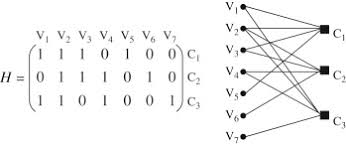
\includegraphics[width=0.7\textwidth]{./pic/Tanner Graph}}
    \caption{ Tanner Graph}
    \label{fig:Tanner Graph}
\end{figure}\cite{Tannerg} 

Die \autoref{fig:Tanner Graph} zeigt die variablen Knoten $V_j$  mit $j\in \left\{1, 2, 3, 4, 5, 6, 7\right\}$ und $C_k$ Prüfknoten mit $k\in \left\{1, 2, 3\right\}$.\\

\begin{Beispiel}[Der weiche Entscheidungsdekodieralgorithmus]
Angenommen, das Codewort $c$ wird gesendet und $y = c + e$ wird empfangen, wobei $e$ der unbekannte Fehlervektor ist. Angesichts des Syndroms $Hy^\intercal = He^\intercal = z^\intercal$ besteht das Ziel des dekodieres darin,\\ 

$prob(ek = 1 \mid z)$ für $1 \leq k \leq n$ zu berechnen.\\

Der Algorithmus berechnet iterativ zwei Wahrscheinlichkeiten für jede Kante des Tanner-Graphen und jedes $e\in \left\{0, 1\right\}$. 
Wenn der Graph Zyklen hat, sind diese Wahrscheinlichkeiten Annäherungen an\\

$prob(ek = 1 \mid z)$ für $1 \leq k \leq n$.\\

Letzten Endes ist es egal, wie diese Wahrscheinlichkeiten genau lauten; es geht nur darum, eine Lösung für $He^\intercal = z^\intercal$ zu erhalten.
Daher kann der Algorithmus auch dann erfolgreich eingesetzt werden, wenn lange Zyklen vorhanden sind.\cite[S. 11]{huffman}\\
\end{Beispiel}

% ----------------------------
\section{Vergleich von LDPC-Codes gegenüber herkömmlichen Blockcodes} 
% ----------------------------

\begin{Beispiel}[Vergleich von LDPC-Codes gegenüber herkömmlichen Blockcodes]

Bei LDPC - Codes werden, wie bei allen Blockcodes, den informationstragenden Bits zusätzliche Bits hinzugefügt. 
Diese zusätzlichen Bits, die als Paritätsbits bezeichnet werden, bilden zusammen mit den Informationsbits Paritätsgleichungen. 
Bei einer fehlerfreien Übertragung müssen diese Gleichungen bei einer  Paritätsprüfung null ergeben, dargestellt durch $Hc^\intercal=0$.\\

Ein Unterschied zu traditionellen Blockcodes liegt in der Dekodierungsmethode.
Klassische Blockcodes werden in einem einzigen Durchlauf dekodiert, während LDPC-Codes iterative Verfahren nutzen.\\

Ein zusätzlicher Unterschied ist, dass LDPC-Codes durch ihre Kontroll- Paritätsprüfmatrix charakterisiert sind und nicht, wie bei herkömmlichen Blockcodes, durch ihre Generatormatrix.
\end{Beispiel}

    

\chapter{Definition von Turbo Codes}
% ----------------------------

\autoref{fig:Codierungsgewinn in der Satellitenkommunikation} beschreibt die Turbocodierung, annhand vier Turbocodes, mit  satelliten Kommunikationspaketen. Der Wert von \(m\) ist die Nachrichtenlänge.\cite[S. 7]{huffman}

\begin{figure}[!ht]
    \centering
     {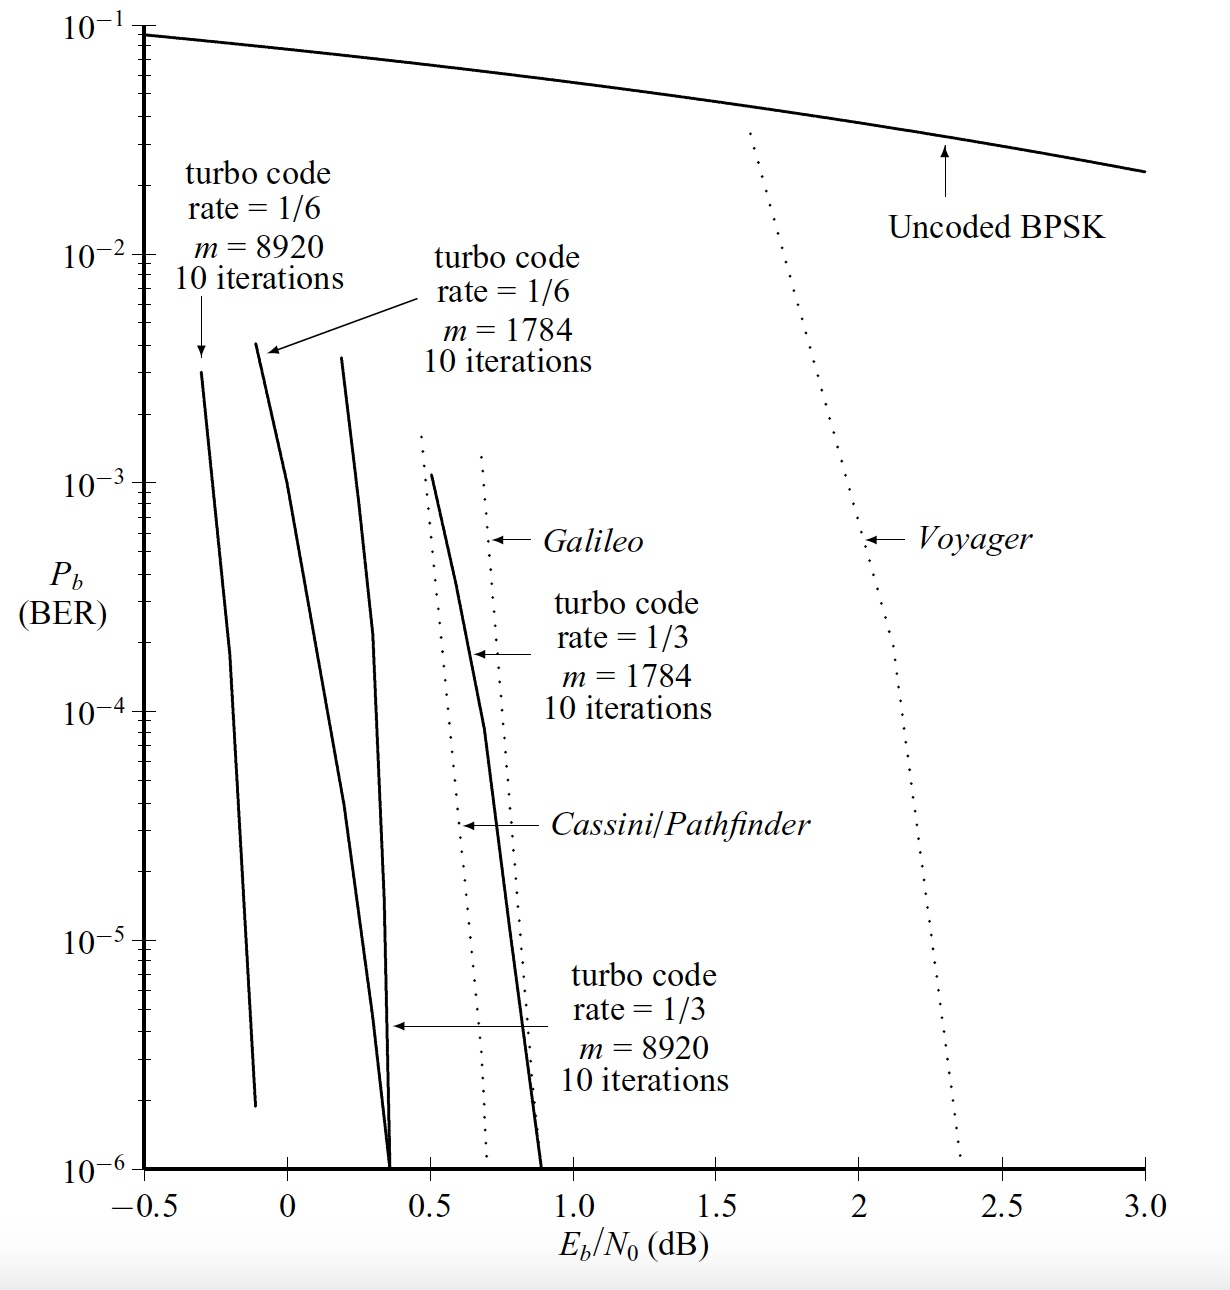
\includegraphics[width=0.7\textwidth]{./pic/Codierungsgewinn in der Satellitenkommunikation}}
    \caption{ Codierungsgewinn in der Satellitenkommunikation}
    \label{fig:Codierungsgewinn in der Satellitenkommunikation}
\end{figure} 
\autoref{fig:Codierungsgewinn in der Satellitenkommunikation}

In \autoref{fig:kommunikationskanal}
wird gezeigt, 
dass ein Ziel der Kodierung darin besteht, mit Signal-Rausch-Verhältnissen nahe der 
Shannon-Grenze zu kommunizieren. 
\autoref{fig:Codierungsgewinn in der Satellitenkommunikation}
zeigt den Vergleich zwischen dem Signal-Rausch-Verhältnis 
Eb/N0 und der Bitfehlerrate Pb der in einigen Satelliten Kommunikationspaketen 
verwendeten Codes.
\pagebreak

\begin{definition}[parallel verketteter Code]
Ein parallel verketteter Code besteht aus zwei oder mehr Komponenten-Codes, 
bei denen es sich in der Regel entweder um 
binäre Faltungscodes oder um Blockcodes mit einer Trellis-Struktur handelt, 
die zu einer effizienten Dekodierung mit weichen Entscheidungen führt.\\

Wenn die
Komponentencodes des parallel verketteten Codes faltbar sind, wird der resultierende Code als parallel
verketteter Faltungscode oder PCCC bezeichnet. Der Komponentencode hat die Coderate $1/2$, da jedes Nachrichtenbit zwei Codewortbits erzeugt.\\

Im einfachsten Fall, 
handelt es sich um zwei Komponenten-Codes, $C_1$ und $C_2$, 
mit jeweils systematischen Kodierern. Tatsächlich können die Kodierer 
für die beiden Codes identisch sein. \cite[S. 8]{huffman}
\\ 
\end{definition}


\begin{Beispiel}[parallel verketteter Code]
Angenommen, es Existieren Komponentencodes $C_i$ zu einem $[n, n/2]$ Binär-
blockcode mit der Generatormatrix $G_i$ = $[I_{n/2} \quad A_{i}]$, die als Kodierer bezeichnet werden.\\

Bei der vorgehnsweise wendet man die übliche Kodierung an, bei der die Nachricht mit
$xG_i$ kodiert wird. Ein Kodierer für den parallel-verketteten Code mit den Komponenten-Kodierern $xG_1$ und $xG_2$
wird wie folgt gebildet.\\

Die Nachricht $x$ wird mit dem ersten Code kodiert, um $(x, c_1)$ zu erzeugen, wobei $c_1 = xG_1$ ist, wenn der Code ein Blockcode ist. Als nächstes wird die Nachricht $x$ an einen Permuter, auch Interleaver genannt,
weitergeleitet. Der Permuter wendet eine feste Permutation auf die Koordinaten von $x$ an und erzeugt die permutierte Nachricht $\bar{x}$. Die permutierte Nachricht $\bar{x}$ wird mit $G_2$ kodiert, um $(\bar{x}, c_2)$ zu erzeugen, wobei $c_2 = \bar{x}G_2$.\\

Das Codewort, dass an den Kanal weitergegeben wird, ist eine verschachtelte Version der ursprünglichen Nachricht $x$ und der beiden Redundanzzeichenfolgen $c_1$ und $c_2$, die durch die Codes $C_1$ und $C_2$ erzeugt
wurden.\\

Dieser Vorgang ist in im nächstes Abschnitt in
\autoref{fig:Parallel verketteter Code mit zwei Komponenten} dargestellt und wird anhand einer mathematischen Aufgabe genauer erläutert.\\
\end{Beispiel}
\pagebreak

% ----------------------------
\section{Beispielmodell: Ein parallel verketteter Code}
% ---------------------------- 

\begin{Beispiel}[parallel verketteter Code]
Seien $C_1$ und $C_2$ jeweils der erweiterte $[8, 4, 4]$ Hamming-Code mit Generatormatrix


$G_{1}=G_2=\left( \begin{array}{rrrrrrrr}
    1 & 0 & 0 & 0 & 0 & 1 & 1 & 1 \\
    0 & 1 & 0 & 0 & 1 & 0 & 1 & 1 \\
    0 & 0 & 1 & 0 & 1 & 1 & 0 & 1 \\
    0 & 0 & 0 & 1 & 1 & 1 & 1 & 0 \\
   \end{array}\right). 
$\\

Angenommen, der Permuter ist durch die Permutation $(1,\quad 3)(2,\quad 4)$ gegeben.

Die zu kodierende Nachricht ist beispielsweise $x = (1,0,1,1).$ Dann ist $xG_1 = (1,0,1,1,0,1,0,0)$ und   $c_1 = (0,1,0,0)$. Die permutierte Nachricht ist $\bar{x} = (1,1,1,0)$, die als $\bar{x}G_2 = (1,1,1,0,0,0,0,1)$ kodiert wird und $c_2 = (0,0,0,1)$ ergibt.


\begin{figure}[!ht]
    \centering
     {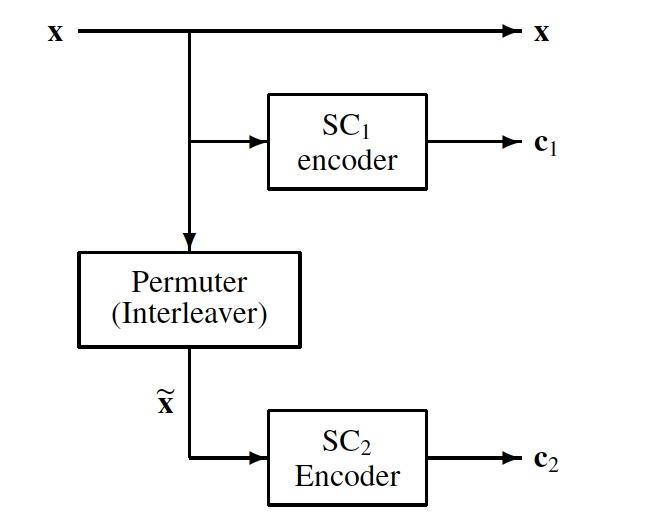
\includegraphics[width=0.7\textwidth]{./pic/Parallel verketteter Code mit zwei Komponenten}}
    \caption{ Parallel verketteter Code mit zwei Komponenten}
    \label{fig:Parallel verketteter Code mit zwei  Komponenten}
\end{figure} 

Dann wird $(x, c_1, c_2) = ((1,0,1,1), (0,1,0,0), (0,0,0,1))$ in verschachtelter Form übertragen, wobei die ersten Bits von $x, c_1, c_2$, gefolgt werden von den zweiten Bits, dritten Bits und vierten Bits, als $((1,0,0), (0,1,0), (1,0,0), (1,0,1)).$\\

In der \autoref{fig:Parallel verketteter Code mit zwei Komponenten} zeigen $SC_1$ und $SC_2$, 
dass die Kodierer in Standardform vorliegen. 
Der resultierende parallel verkettete Code hat die Coderate von $1/3$.
\end{Beispiel} \cite[S. 9]{huffman}
\pagebreak

\begin{Beispiel}[parallel verketteter Code]
    Finde die Permuter Form aller $16$ Codewörter des in Beispielaufgabe $a$ beschriebenen parallel verketteten Codes und bestimme den minimalen Abstand des resultierenden $[12, 4]$ Binärcodes.\\
    
    Um die Aufgabe zu Lösen, geht man schrittweise vor:
    
    Zu einem $[8, 4, 4]$ Hamming-Code findet man alle $2^4 = 16$ empfangenen Nachrichten $x$, da der Code vier Informationsbits aufweist.
    
    Die $16$ möglichen $x$ Nachrichten sind:\\
    
    $x_1= (0,0,0,0)$
    
    $x_2= (0,0,0,1)$
    
    $x_3= (0,0,1,0)$ 
    
    $x_4= (0,1,0,0)$ 
    
    $x_5= (1,0,0,0)$ 
    
    $x_6= (0,0,1,1)$ 
    
    $x_7= (0,1,0,1)$ 
    
    $x_8= (1,0,0,1)$ 
    
    $x_9= (0,1,1,0)$ 
    
    $x_{10}= (1,0,1,0)$ 
    
    $x_{11}= (1,1,0,0)$ 
    
    $x_{12}= (0,1,1,1)$ 
    
    $x_{13}= (1,1,1,0)$ 
    
    $x_{14}= (1,1,0,1)$ 
    
    $x_{15}= (1,0,1,1)$ 
    
    $x_{16}= (1,1,1,1)$\\
    \pagebreak
    
    Durch Multiplikation dieser $16$ Nachricht mit $xG_1$ erhält man die Codewörter $c_1$.\\
    
    $x_1G_1= (0,0,0,0,0,0,0,0) \Rightarrow c_1= (0,0,0,0)$
    
    $x_2G_1= (0,0,0,1,1,1,1,0) \Rightarrow c_1= (1,1,1,0)$
    
    $x_3G_1= (0,0,1,0,1,1,0,1) \Rightarrow c_1= (1,1,0,1)$
    
    $x_4G_1= (0,1,0,0,1,0,1,1) \Rightarrow c_1= (1,0,1,1)$
    
    $x_5G_1= (1,0,0,0,0,1,1,1) \Rightarrow c_1= (0,1,1,1)$
    
    $x_6G_1= (0,0,1,1,2,2,1,1) \bmod 2 = (0,0,1,1,0,0,1,1) \Rightarrow c_1= (0,0,1,1)$
    
    $x_7G_1= (0,1,0,1,2,1,2,1) \bmod 2 = (0,1,0,1,0,1,0,1) \Rightarrow c_1= (0,1,0,1)$
    
    $x_8G_1= (1,0,0,1,1,2,2,1) \bmod 2 = (1,0,0,1,1,0,0,1) \Rightarrow c_1= (1,0,0,1)$
    
    $x_9G_1= (0,1,1,0,2,1,1,2) \bmod 2 = (0,1,1,0,0,1,1,0) \Rightarrow c_1= (0,1,1,0)$
    
    $x_{10}G_1= (1,0,1,0,1,2,1,2) \bmod 2 = (1,0,1,0,1,0,1,0) \Rightarrow c_1= (1,0,1,0)$
    
    $x_{11}G_1= (1,1,0,0,1,1,2,2) \bmod 2 = (1,1,0,0,1,1,0,0) \Rightarrow c_1= (1,1,0,0)$
    
    $x_{12}G_1= (0,1,1,1,3,2,2,2) \bmod 2 = (0,1,1,1,1,0,0,0) \Rightarrow c_1= (1,0,0,0)$
    
    $x_{13}G_1= (1,1,1,0,2,2,2,3) \bmod 2 = (1,1,1,0,0,0,0,1) \Rightarrow c_1= (0,0,0,1)$
    
    $x_{14}G_1= (1,1,0,1,2,2,3,2) \bmod 2 = (1,1,0,1,0,0,1,0) \Rightarrow c_1= (0,0,1,0)$
    
    $x_{15}G_1= (1,0,1,1,2,3,2,2) \bmod 2 = (1,0,1,1,0,1,0,0) \Rightarrow c_1= (0,1,0,0)$
    
    $x_{16}G_1= (1,1,1,1,3,3,3,3) \bmod 2 = (1,1,1,1,1,1,1,1) \Rightarrow c_1= (1,1,1,1)$\\
    
    Die Permutation $(1,\quad 3)(2,\quad 4)$ tauscht die ersten beiden Bits der Nachricht $x$ mit den dritten und vierten Bits.\\
    Angenommen, es existiert eine Nachricht $x$ mit vier Bits $x = (a,b,c,d)$\\
    
    $(1,\quad 3)$: Bit $a$ wird mit dem dritten Bit $c$ getauscht.
    
    $(2,\quad 4)$: Bit $b$ wird mit dem vierten Bit $d$ getauscht.
    
    Dies führt zu einer permutierten neuen Nachricht $\bar{x}=(c,d,a,b).$\\
    
    Die Nachricht $x_1= (0,0,0,0)$ und $x_{16}=(1,1,1,1)$\\ bleiben unverändert, da alle Bits gleich sind.\\
    
    Die Nachricht $x_{15}=(1,0,1,1)$:\\
    Ursprüngliche Form: $(a= 1, b=0, c=1, d=1)$\\
    Nach Permutation: $\bar{x}_{15}=(c,d,a,b)=(1,1,1,0)$\\
    
    Die Nachricht $x_9= (0,1,1,0):$\\
    Ursprüngliche Form: $(a=0, b=1, c=1, d=0)$\\
    Nach Permutation: $\bar{x}_{9}=(c,d,a,b)=(1,0,0,1)$\\
    \pagebreak

    Angewandt auf alle $16$ möglichen Empfangenen Nachrichten $x$ erhält man:\\
    
    $x_1= (0,0,0,0) \Rightarrow \bar{x}_{1} = (0,0,0,0)$
    
    $x_2= (0,0,0,1) \Rightarrow \bar{x}_{2} = (0,1,0,0)$
    
    $x_3= (0,0,1,0) \Rightarrow \bar{x}_{3} = (1,0,0,0)$
    
    $x_4= (0,1,0,0) \Rightarrow \bar{x}_{4} = (0,0,0,1)$
    
    $x_5= (1,0,0,0) \Rightarrow \bar{x}_{5} = (0,0,1,0)$
    
    $x_6= (0,0,1,1) \Rightarrow \bar{x}_{6} = (1,1,0,0)$
    
    $x_7= (0,1,0,1) \Rightarrow \bar{x}_{7} = (0,1,0,1)$
    
    $x_8= (1,0,0,1) \Rightarrow \bar{x}_{8} = (0,1,1,0)$
    
    $x_9= (0,1,1,0) \Rightarrow \bar{x}_{9} = (1,0,0,1)$
    
    $x_{10}= (1,0,1,0) \Rightarrow \bar{x}_{10} = (1,0,1,0)$
    
    $x_{11}= (1,1,0,0) \Rightarrow \bar{x}_{11} = (0,0,1,1)$
    
    $x_{12}= (0,1,1,1) \Rightarrow \bar{x}_{12} = (1,1,0,1)$
    
    $x_{13}= (1,1,1,0) \Rightarrow \bar{x}_{13} = (1,0,1,1)$
    
    $x_{14}= (1,1,0,1) \Rightarrow \bar{x}_{14} = (0,1,1,1)$
    
    $x_{15}= (1,0,1,1) \Rightarrow \bar{x}_{15} = (1,1,1,0)$
    
    $x_{16}= (1,1,1,1) \Rightarrow \bar{x}_{16} = (1,1,1,1)$\\
    
    Durch Multiplikation dieser permutierten Nachrichten mit  $\bar{x}G_2$ erhält man die Codewörter $c_2$:\\
    
    $\bar{x}_{1}G_2= (0,0,0,0,0,0,0,0) \Rightarrow c_2= (0,0,0,0)$
    
    $\bar{x}_{2}G_2= (0,1,0,0,1,0,1,1) \Rightarrow c_2= (1,0,1,1)$
    
    $\bar{x}_{3}G_2= (1,0,0,0,0,1,1,1) \Rightarrow c_2= (0,1,1,1)$
    
    $\bar{x}_{4}G_2= (0,0,0,1,1,1,1,0) \Rightarrow c_2= (1,1,1,0)$
    
    $\bar{x}_{5}G_2= (0,0,1,0,1,1,0,1) \Rightarrow c_2= (1,1,0,1)$
    
    $\bar{x}_{6}G_2= (1,1,0,0,1,1,2,2) \bmod 2 = (1,1,0,0,1,1,0,0) \Rightarrow c_2= (1,1,0,0)$
    
    $\bar{x}_{7}G_2= (0,1,0,1,2,1,2,1) \bmod 2 = (0,1,0,1,0,1,0,1) \Rightarrow c_2= (0,1,0,1)$
    
    $\bar{x}_{8}G_2= (0,1,1,0,2,1,1,2) \bmod 2 = (0,1,1,0,0,1,1,0) \Rightarrow c_2= (0,1,1,0)$
    
    $\bar{x}_{9}G_2= (1,0,0,1,1,2,2,1) \bmod 2 = (1,0,0,1,1,0,0,1) \Rightarrow c_2= (1,0,0,1)$
    
    $\bar{x}_{10}G_2= (1,0,1,0,1,2,1,2) \bmod 2 = (1,0,1,0,1,0,1,0) \Rightarrow c_2= (1,0,1,0)$
    
    $\bar{x}_{11}G_2= (0,0,1,1,2,2,1,1) \bmod 2 = (0,0,1,1,0,0,1,1) \Rightarrow c_2= (0,0,1,1)$
    
    $\bar{x}_{12}G_2= (1,1,0,1,2,2,3,2) \bmod 2 = (1,1,0,1,0,0,1,0) \Rightarrow c_2= (0,0,1,0)$
    
    $\bar{x}_{13}G_2= (1,0,1,1,2,3,2,2) \bmod 2 = (1,0,1,1,0,1,0,0) \Rightarrow c_2= (0,1,0,0)$
    
    $\bar{x}_{14}G_2= (0,1,1,1,3,2,2,2) \bmod 2 = (0,1,1,1,1,0,0,0) \Rightarrow c_2= (1,0,0,0)$
    
    $\bar{x}_{15}G_2= (1,1,1,0,2,2,2,3) \bmod 2 = (1,1,1,0,0,0,0,1) \Rightarrow c_2= (0,0,0,1)$
    
    $\bar{x}_{16}G_2= (1,1,1,1,3,3,3,3) \bmod 2 = (1,1,1,1,1,1,1,1) \Rightarrow c_2= (1,1,1,1)$\\
    \pagebreak
    
    Für jede der $16$ Nachrichten $x$ und jedes Paar $(c_1,c_2)$ erhält man die verschachtelte Form $(x,c_1,c_2):$\\
    
    $(x_1, c_1, c_2) = (0,0,0,0, 0,0,0,0, 0,0,0,0)$
    
    
    $(x_2, c_1, c_2) = (0,0,0,1, 1,1,1,0, 1,0,1,1)$
    
    
    $(x_3, c_1, c_2) = (0,0,1,0, 1,1,0,1, 0,1,1,1)$
    
    
    $(x_4, c_1, c_2) = (0,1,0,0, 1,0,1,1, 1,1,1,0)$
    
    
    $(x_5, c_1, c_2) = (1,0,0,0, 0,1,1,1, 1,1,0,1)$
    
    
    $(x_6, c_1, c_2) = (0,0,1,1, 0,0,1,1, 1,1,0,0)$
    
    
    $(x_7, c_1, c_2) = (0,1,0,1, 0,1,0,1, 0,1,0,1)$
    
    
    $(x_8, c_1, c_2) = (1,0,0,1, 1,0,0,1, 0,1,1,0)$
    
    
    $(x_9, c_1, c_2) = (0,1,1,0, 0,1,1,0, 1,0,0,1)$
    
    
    $(x_{10}, c_1, c_2) = (1,0,1,0, 1,0,1,0, 1,0,1,0)$
    
    
    $(x_{11}, c_1, c_2) = (1,1,0,0, 1,1,0,0, 0,0,1,1)$
    
    
    $(x_{12}, c_1, c_2) = (0,1,1,1, 1,0,0,0, 0,0,1,0)$
    
    
    $(x_{13}, c_1, c_2) = (1,1,1,0, 0,0,0,1, 0,1,0,0)$
    
    
    $(x_{14}, c_1, c_2) = (1,1,0,1, 0,0,1,0, 1,0,0,0)$
    
    
    $(x_{15}, c_1, c_2) = (1,0,1,1, 0,1,0,0, 0,0,0,1)$
     
    
    $(x_{16}, c_1, c_2) = (1,1,1,1, 1,1,1,1, 1,1,1,1)$\\
    
    Die verschachtelte Form $(x,c_1,c_2)$ kombiniert einige Bits aus der ursprünglichen Nachricht $x$, den ursprünglichen Codewörtern $c_1$ und den permutierten Codewörtern $c_2$ und ordnet sie wie folgt an, um sie schlie\ss{}lich als neues kodiertes Codewort mit wahrscheinlich unterschiedlichen Bits an denselben Stellen, also mit einen bestimmten Hamming-Abstand, zu übertragen:\\
    
    Ordnungsalgorithmus:\\
    
    $x= (a,b,c,d) \quad c_1= (e,f,g,h) \quad c_2= (i,j,k,l)\quad (x,c_1,c_2)= ((a,b,c,d), (e,f,g,h), (i,j,k,l))$\\
    
    Die erste Anordnung ordnet die ersten Bits von:\\
    $(x,c_1,c_2) = ((a,b,c,d), (e,f,g,h), (i,j,k,l)) = (a,e,i)$\\
    
    Die zweite Anordnung ordnet die zweiten Bits von:\\
    $(x,c_1,c_2) = ((a,b,c,d), (e,f,g,h), (i,j,k,l)) = ((a,e,i), (b,f,j))$\\
    
    Die letzte Anordnung ordnet die dritten und vierten Bits von:\\
    $(x,c_1,c_2) = ((a,b,c,d), (e,f,g,h), (i,j,k,l)) = ((a,e,i), (b,f,j),(c,g,k), (d,h,l))$\\ 
    
    Wendet man diesen Ordnungsalgorithmus auf alle $16$ verschachtelten Formen an erhält man:\\
    
    
    $(x_{1}, c_1, c_2) = ((0,0,0,0), (0,0,0,0), (0,0,0,0)) \Rightarrow$ Ordnungsalgorithmus: $((0,0,0),(0, 0,0),(0,0, 0),(0,0,0))$ mit Abstand $0$.\\
    
    $(x_{2}, c_1, c_2) = ((0,0,0,1), (1,1,1,0), (1,0,1,1)) \Rightarrow$ Ordnungsalgorithmus: $((0,1,1),(0, 1,0),(0,1, 1),(1,0,1))$ mit Abstand $8$.\\
    \pagebreak
    
    $(x_{3}, c_1, c_2) = ((0,0,1,0), (1,1,0,1), (0,1,1,1)) \Rightarrow$ Ordnungsalgorithmus: $((0,1,0),(0, 1,1),(1,0, 1),(0,1,1))$ mit Abstand $6$.\\
    
    $(x_{4}, c_1, c_2) = ((0,1,0,0), (1,0,1,1), (1,1,1,0)) \Rightarrow$ Ordnungsalgorithmus: $((0,1,1),(1, 0,1),(0,1, 1),(0,1,0))$ mit Abstand $6$.\\
    
    $(x_{5}, c_1, c_2) = ((1,0,0,0), (0,1,1,1), (1,1,0,1)) \Rightarrow$ Ordnungsalgorithmus: $((1,0,1),(0, 1,1),(0,1, 0),(0,1,1))$ mit Abstand $6$.\\
    
    $(x_{6}, c_1, c_2) = ((0,0,1,1), (0,0,1,1), (1,1,0,0)) \Rightarrow$ Ordnungsalgorithmus: $((0,0,1),(0, 0,1),(1,1, 0),(1,1,0))$ mit Abstand $4$.\\
    
    $(x_{7}, c_1, c_2) = ((0,1,0,1), (0,1,0,1), (0,1,0,1)) \Rightarrow$ Ordnungsalgorithmus: $((0,0,0),(1, 1,1),(0,0, 0),(1,1,1))$ mit Abstand $4$.\\
    
    $(x_{8}, c_1, c_2) = ((1,0,0,1), (1,0,0,1), (0,1,1,0)) \Rightarrow$ Ordnungsalgorithmus: $((1,1,0),(0, 0,1),(0,0, 1),(1,1,0))$ mit Abstand $6$.\\
    
    $(x_{9}, c_1, c_2) = ((0,1,1,0), (0,1,1,0), (1,0,0,1)) \Rightarrow$ Ordnungsalgorithmus: $((0,0,1),(1, 1,0),(1,1, 0),(0,0,1))$ mit Abstand $6$.\\
    
    $(x_{10}, c_1, c_2) = ((1,0,1,0), (1,0,1,0), (0,1,0,1)) \Rightarrow$ Ordnungsalgorithmus: $((1,1,1),(0, 0,0),(1,1, 1),(0,0,0))$ mit Abstand $4$.\\
    
    $(x_{11}, c_1, c_2) = ((1,1,0,0), (1,1,0,0), (0,0,1,1)) \Rightarrow$ Ordnungsalgorithmus: $((1,1,0),(1, 1,0),(0,0, 1),(0,0,1))$ mit Abstand $4$.\\
    
    $(x_{12}, c_1, c_2) = ((0,1,1,1), (1,0,0,0), (0,0,1,0)) \Rightarrow$ Ordnungsalgorithmus: $((0,1,0),(1, 0,0),(1,0, 1),(1,0,0))$ mit Abstand $6$.\\
    
    $(x_{13}, c_1, c_2) = ((1,1,1,0), (0,0,0,1), (0,1,0,0)) \Rightarrow$ Ordnungsalgorithmus: $((1,0,0),(1, 0,1),(1,0, 0),(0,1,0))$ mit Abstand $8$.\\
    
    $(x_{14}, c_1, c_2) = ((1,1,0,1), (0,0,1,0), (1,0,0,0)) \Rightarrow$ Ordnungsalgorithmus: $((1,0,1),(1, 0,0),(0,1 ,0),(1,0,0))$ mit Abstand $6$.\\
    
    $(x_{15}, c_1, c_2) = ((1,0,1,1), (0,1,0,0), (0,0,0,1)) \Rightarrow$ Ordnungsalgorithmus: $((1,0,0),(0, 1,0),(1,0, 0),(1,0,1))$ mit Abstand $6$.\\
    
    $(x_{16}, c_1, c_2) = ((1,1,1,1), (1,1,1,1), (1,1,1,1)) \Rightarrow$ Ordnungsalgorithmus: $((1,1,1),(1, 1,1),(1,1, 1),(1,1,1))$ mit Abstand $6$.\\
    
    
    
    
    
    Um den minimalen Abstand genau zu berechnen, müssten man die Hamming-Abstände aller möglichen Paare der $16$ Codewörter bestimmen und den kleinsten Abstand finden. Zwei verschachtelte Codewörter $(x_{1}, c_1, c_2) = ((0,0,0,0), (0,0,0,0), (0,0,0,0))$ und $(x_{16}, c_1, c_2) = ((1,1,1,1), (1,1,1,1), (1,1,1,1))$ sind nach dem Ordnungsalgorithmus identisch, was zu einem Hamming- Abstand von $0$ führt. Demzufolge scheint es so, dass der Mindestabstand des Codes $[12, 4]$ gleich $0$ beträgt. Dies würde jedoch bedeuten, dass der Code $[12, 4]$ keine Fehlererkennung bietet. Dementsprechend beträgt der minimale Abstand des ursprünglichen Codes $[12, 4]$ gleich $4$.\\
    \pagebreak
    
    Die folgenden verschachtelten Codewörtern weisen den minimalen Hamming-Abstand von $4$ auf und werden erfolgreich übertragen.\\
    
    $(x_{6}, c_1, c_2) = ((0,0,1,1), (0,0,1,1), (1,1,0,0)) \Rightarrow$ Ordnungsalgorithmus: $((0,0,1),(0, 0,1),(1,1, 0),(1,1,0))$ mit Abstand $4$.\\
    
    $(x_{7}, c_1, c_2) = ((0,1,0,1), (0,1,0,1), (0,1,0,1)) \Rightarrow$ Ordnungsalgorithmus: $((0,0,0),(1, 1,1),(0,0, 0),(1,1,1))$ mit Abstand $4$.\\
    
    $(x_{10}, c_1, c_2) = ((1,0,1,0), (1,0,1,0), (0,1,0,1)) \Rightarrow$ Ordnungsalgorithmus: $((1,1,1),(0, 0,0),(1,1, 1),(0,0,0))$ mit Abstand $4$.\\
    
    $(x_{11}, c_1, c_2) = ((1,1,0,0), (1,1,0,0), (0,0,1,1)) \Rightarrow$ Ordnungsalgorithmus: $((1,1,0),(1, 1,0),(0,0, 1),(0,0,1))$ mit Abstand $4$.\\
    
\end{Beispiel}


\begin{Beispiel}[parallel verketteter Code]
    Im folgenden ist der Permuter durch die Permutation $(3,\quad 2)(4,\quad 1)$ gegeben:\\

    Die Permutation $(3,\quad 2)(4,\quad 1)$ tauscht das dritte und zweite Bit der Nachricht $x$ mit den vierten und ersten Bit.\\
    
    Angenommen, eine Nachricht $x$ mit vier Bits $x = (a,b,c,d)$\\
    
    $(3,\quad 2)$ bedeutet: Bit $c$ wird mit dem zweiten Bit $b$ getauscht.\\
    $(4,\quad 1)$ bedeutet: Bit $d$ wird mit dem ersten Bit $a$ getauscht.\\
    
    Dies führt zu einer permutierten neuen Nachricht $\bar{x} = (d,c,b,a).$\\
    Die Nachricht  $x_{1} = (0,0,0,0)$ und  $x_{16} = (1,1,1,1)$  bleiben wie bisher unverändert, da alle Bits gleich sind.\\
    
    
    Die Nachricht $x_{15}=(1,0,1,1)$:\\
    Ursprüngliche Form: $(a= 1, b=0, c=1, d=1)$\\
    Nach Permutation: $\bar{x} = (d,c,b,a)=(1,1,0,1)$\\
    
    Die Nachricht $x_9= (0,1,1,0):$\\
    Ursprüngliche Form: $(a=0, b=1, c=1, d=0)$\\
    Nach Permutation: $\bar{x}_{9}=(d,c,b,a)=(0,1,1,0)$\\
    \pagebreak
    
    Angewandt auf alle $16$ möglichen Empfangenen Nachrichten $x$ erhält man:\\
    
    
    $x_1= (0,0,0,0) \Rightarrow \bar{x}_{1} = (0,0,0,0)$
    
    $x_2= (0,0,0,1) \Rightarrow \bar{x}_{2} = (1,0,0,0)$
    
    $x_3= (0,0,1,0) \Rightarrow \bar{x}_{3} = (0,1,0,0)$
    
    $x_4= (0,1,0,0) \Rightarrow \bar{x}_{4} = (0,0,1,0)$
    
    $x_5= (1,0,0,0) \Rightarrow \bar{x}_{5} = (0,0,0,1)$
    
    $x_6= (0,0,1,1) \Rightarrow \bar{x}_{6} = (1,1,0,0)$
    
    $x_7= (0,1,0,1) \Rightarrow \bar{x}_{7} = (1,0,1,0)$
    
    $x_8= (1,0,0,1) \Rightarrow \bar{x}_{8} = (1,0,0,1)$
    
    $x_9= (0,1,1,0) \Rightarrow \bar{x}_{9} = (0,1,1,0)$
    
    $x_{10}= (1,0,1,0) \Rightarrow \bar{x}_{10} = (0,1,0,1)$
    
    $x_{11}= (1,1,0,0) \Rightarrow \bar{x}_{11} = (0,0,1,1)$
    
    $x_{12}= (0,1,1,1) \Rightarrow \bar{x}_{12} = (1,1,1,0)$
    
    $x_{13}= (1,1,1,0) \Rightarrow \bar{x}_{13} = (0,1,1,1)$
    
    $x_{14}= (1,1,0,1) \Rightarrow \bar{x}_{14} = (1,0,1,1)$
    
    $x_{15}= (1,0,1,1) \Rightarrow \bar{x}_{15} = (1,1,0,1)$
    
    $x_{16}= (1,1,1,1) \Rightarrow \bar{x}_{16} = (1,1,1,1)$\\

    
    Durch Multiplikation dieser permutierten Nachrichten mit  $\bar{x}G_2$ erhält man die Codewörter $c_2$:\\
    
    
    $\bar{x}_{1}G_2= (0,0,0,0,0,0,0,0) \Rightarrow c_2= (0,0,0,0)$
    
    $\bar{x}_{2}G_2= (1,0,0,0,0,1,1,1) \Rightarrow c_2= (0,1,1,1)$
    
    $\bar{x}_{3}G_2= (0,1,0,0,1,0,1,1) \Rightarrow c_2= (1,0,1,1)$
    
    $\bar{x}_{4}G_2= (0,0,1,0,1,1,0,1) \Rightarrow c_2= (1,1,0,1)$
    
    $\bar{x}_{5}G_2= (0,0,0,1,1,1,1,0) \Rightarrow c_2= (1,1,1,0)$
    
    $\bar{x}_{6}G_2= (1,1,0,0,1,1,2,2) \bmod 2 = (1,1,0,0,1,1,0,0) \Rightarrow c_2= (1,1,0,0)$
    
    $\bar{x}_{7}G_2= (1,0,1,0,1,2,1,2) \bmod 2 = (1,0,1,0,1,0,1,0 ) \Rightarrow c_2= (1,0,1,0)$
    
    $\bar{x}_{8}G_2= (1,0,0,1,1,2,2,1) \bmod 2 = (1,0,0,1,1,0,0,1) \Rightarrow c_2= (1,0,0,1)$
    
    $\bar{x}_{9}G_2= (0,1,1,0,2,1,1,2) \bmod 2 = (0,1,1,0,0,1,1,0) \Rightarrow c_2= (0,1,1,0)$
    
    $\bar{x}_{10}G_2= (0,1,0,1,2,1,2,1) \bmod 2 = (0,1,0,1,0,1,0,1) \Rightarrow c_2= (0,1,0,1)$
    
    $\bar{x}_{11}G_2= (0,0,1,1,2,2,1,1) \bmod 2 = (0,0,1,1,0,0,1,1) \Rightarrow c_2= (0,0,1,1)$
    
    $\bar{x}_{12}G_2= (1,1,1,0,2,2,2,3) \bmod 2 = (1,1,1,0,0,0,0,1) \Rightarrow c_2= (0,0,0,1)$
    
    $\bar{x}_{13}G_2= (0,1,1,1,3,2,2,2) \bmod 2 = (0,1,1,1,1,0,0,0) \Rightarrow c_2= (1,0,0,0)$
    
    $\bar{x}_{14}G_2= (1,0,1,1,2,3,2,2) \bmod 2 = (1,0,1,1,0,1,0,0) \Rightarrow c_2= (0,1,0,0)$
    
    $\bar{x}_{15}G_2= (1,1,0,1,2,2,3,2) \bmod 2 = (1,1,0,1,0,0,1,0) \Rightarrow c_2= (0,0,1,0)$
    
    $\bar{x}_{16}G_2= (1,1,1,1,3,3,3,3) \bmod 2 = (1,1,1,1,1,1,1,1) \Rightarrow c_2= (1,1,1,1)$\\
    \pagebreak
    
    Für jede der $16$ Nachrichten $x$ und jedes Paar $(c_1,c_2)$ erhält man die verschachtelte Form $(x,c_1,c_2):$\\
    
    $(x_1, c_1, c_2) = ((0,0,0,0), (0,0,0,0), (0,0,0,0))$
    
    $(x_2, c_1, c_2) = ((0,0,0,1), (1,1,1,0), (0,1,1,1))$
    
    $(x_3, c_1, c_2) = ((0,0,1,0), (1,1,0,1), (1,0,1,1))$
    
    $(x_4, c_1, c_2) = ((0,1,0,0), (1,0,1,1), (1,1,0,1))$
    
    $(x_5, c_1, c_2) = ((1,0,0,0), (0,1,1,1), (1,1,1,0))$
    
    $(x_6, c_1, c_2) = ((0,0,1,1), (0,0,1,1), (1,1,0,0))$
    
    $(x_7, c_1, c_2) = ((0,1,0,1), (0,1,0,1), (1,0,1,0))$
    
    $(x_8, c_1, c_2) = ((1,0,0,1), (1,0,0,1), (1,0,0,1))$
    
    $(x_9, c_1, c_2) = ((0,1,1,0), (0,1,1,0), (0,1,1,0))$
    
    $(x_{10}, c_1, c_2) = ((1,0,1,0), (1,0,1,0), (0,1,0,1))$
    
    $(x_{11}, c_1, c_2) = ((1,1,0,0), (1,1,0,0), (0,0,1,1))$
    
    $(x_{12}, c_1, c_2) = ((0,1,1,1), (1,0,0,0), (0,0,0,1))$
    
    $(x_{13}, c_1, c_2) = ((1,1,1,0), (0,0,0,1), (1,0,0,0))$
    
    $(x_{14}, c_1, c_2) = ((1,1,0,1), (0,0,1,0), (0,1,0,0))$
    
    $(x_{15}, c_1, c_2) = ((1,0,1,1), (0,1,0,0), (0,0,1,0))$
    
    $(x_{16}, c_1, c_2) = ((1,1,1,1), (1,1,1,1), (1,1,1,1))$\\
    
    Die verschachtelte Form $(x,c_1,c_2)$ kombiniert einige Bits aus der ursprünglichen Nachricht $x$, den ursprünglichen Codewörtern $c_1$ und den permutierten Codewörtern $c_2$ und ordnet sie mit Hilfe eines Ordnungsalgorithmus an.\\
    Wendet man diesen Ordnungsalgorithmus auf alle $16$ verschachtelten Formen an erhält man:\\
    
    
    $(x_{1}, c_1, c_2) = ((0,0,0,0), (0,0,0,0), (0,0,0,0)) \Rightarrow$ Ordnungsalgorithmus: $((0,0,0),(0, 0,0),(0,0, 0),(0,0,0))$ mit Abstand $0$.\\
    
    $(x_{2}, c_1, c_2) = ((0,0,0,1), (1,1,1,0), (0,1,1,1)) \Rightarrow$ Ordnungsalgorithmus: $((0,1,0),(0, 1,1),(0,1, 1),(1,0,1))$ mit Abstand $0$.\\
    
    $(x_{3}, c_1, c_2) = ((0,0,1,0), (1,1,0,1), (1,0,1,1)) \Rightarrow$ Ordnungsalgorithmus: $((0,1,1),(0, 1,0),(1,0, 0),(0,1,1))$ mit Abstand $5$.\\
    
    $(x_{4}, c_1, c_2) = ((0,1,0,0), (1,0,1,1), (1,1,0,1)) \Rightarrow$ Ordnungsalgorithmus: $((0,1,1),(1, 0,1),(0,1, 0),(0,1,1))$ mit Abstand $8$.\\
    
    $(x_{5}, c_1, c_2) = ((1,0,0,0), (0,1,1,1), (1,1,1,0)) \Rightarrow$ Ordnungsalgorithmus: $((1,0,1),(0, 1,1),(0,1, 1),(0,1,0))$ mit Abstand $4$.\\
    
    $(x_{6}, c_1, c_2) = ((0,0,1,1), (0,0,1,1), (1,1,0,0)) \Rightarrow$ Ordnungsalgorithmus: $((0,0,1),(0, 0,1),(1,1, 0),(1,1,0))$ mit Abstand $4$.\\
    
    $(x_{7}, c_1, c_2) = ((0,1,0,1), (0,1,0,1), (1,0,1,0)) \Rightarrow$ Ordnungsalgorithmus: $((0,0,1),(1, 1,0),(0,0, 1),(1,1,0))$ mit Abstand $6$.\\
    
    $(x_{8}, c_1, c_2) = ((1,0,0,1), (1,0,0,1), (1,0,0,1)) \Rightarrow$ Ordnungsalgorithmus: $((1,1,1),(0, 0,0),(0,0, 0),(1,1,1))$ mit Abstand $8$.\\
    
    $(x_{9}, c_1, c_2) = ((0,1,1,0), (0,1,1,0), (0,1,1,0)) \Rightarrow$ Ordnungsalgorithmus: $((0,0,0),(1, 1,1),(1,1, 1),(0,0,0))$ mit Abstand $8$.\\
    
    $(x_{10}, c_1, c_2) = ((1,0,1,0), (1,0,1,0), (0,1,0,1)) \Rightarrow$ Ordnungsalgorithmus: $((1,1,0),(0, 0,1),(1,1, 0),(0,0,1))$ mit Abstand $6$.\\
    
    $(x_{11}, c_1, c_2) = ((1,1,0,0), (1,1,0,0), (0,0,1,1)) \Rightarrow$ Ordnungsalgorithmus: $((1,1,0),(1, 1,0),(0,0, 1),(0,0,1))$ mit Abstand $4$.\\
    
    $(x_{12}, c_1, c_2) = ((0,1,1,1), (1,0,0,0), (0,0,0,1)) \Rightarrow$ Ordnungsalgorithmus: $((0,1,0),(1, 0,0),(1,0, 0),(1,0,1))$ mit Abstand $4$.\\
    
    $(x_{13}, c_1, c_2) = ((1,1,1,0), (0,0,0,1), (1,0,0,0)) \Rightarrow$ Ordnungsalgorithmus: $((1,0,1),(1, 0,0),(1,0, 0),(0,1,0))$ mit Abstand $6$.\\
    
    $(x_{14}, c_1, c_2) = ((1,1,0,1), (0,0,1,0), (0,1,0,0)) \Rightarrow$ Ordnungsalgorithmus: $((1,0,0),(1, 0,1),(0,1, 0),(1,0,0))$ mit Abstand $5$.\\
    
    $(x_{15}, c_1, c_2) = ((1,0,1,1), (0,1,0,0), (0,0,1,0)) \Rightarrow$ Ordnungsalgorithmus: $((1,0,0),(0, 1,0),(1,0, 1),(1,0,0))$ mit Abstand $8$.\\
    
    $(x_{16}, c_1, c_2) = ((1,1,1,1), (1,1,1,1), (1,1,1,1)) \Rightarrow$ Ordnungsalgorithmus: $((1,1,1), (1, 1,1),(1,1, 1),(1,1,1))$ mit Abstand $0$.\\
    
    
    Die folgenden verschachtelten Codewörtern weisen den minimalen Hamming-Abstand von $4$ auf und werden erfolgreich übertragen.\\
    
    
    
    $(x_{5}, c_1, c_2) = ((1,0,0,0), (0,1,1,1), (1,1,1,0)) \Rightarrow$ Ordnungsalgorithmus: $((1,0,1),(0, 1,1),(0,1, 1),(0,1,0))$ mit Abstand $4$.\\
    
    $(x_{6}, c_1, c_2) = ((0,0,1,1), (0,0,1,1), (1,1,0,0)) \Rightarrow$ Ordnungsalgorithmus: $((0,0,1),(0, 0,1),(1,1, 0),(1,1,0))$ mit Abstand $4$.\\
    
    $(x_{11}, c_1, c_2) = ((1,1,0,0), (1,1,0,0), (0,0,1,1)) \Rightarrow$ Ordnungsalgorithmus: $((1,1,0),(1, 1,0),(0,0, 1),(0,0,1))$ mit Abstand $4$.\\
    
    $(x_{12}, c_1, c_2) = ((0,1,1,1), (1,0,0,0), (0,0,0,1)) \Rightarrow$ Ordnungsalgorithmus: $((0,1,0),(1, 0,0),(1,0, 0),(1,0,1))$ mit Abstand $4$.\\
    
    
    Somit besitzt der $[12, 4]$ Code für die beiden Permutation $(3,\quad 2)(4,\quad 1)$ und $(1,\quad 3)(2,\quad 4)$ den selben minimalen Hamming-Abstand.
    
\end{Beispiel}
\pagebreak

% ----------------------------
\section{Vergleich von  LDPC-Codes  gegenüber Turbo Codes}
% ---------------------------- 
\begin{Beispiel}[Vorteile und Nachteile von LDPC-Codes]
Vorteile von LDPC-Codes:\\

Keine Trellis Struktur notwendig.

Es gibt mehrere Dekodiervarianten.

Man brauch keine langen Permuter Formen, um eine gute Fehlerkorrektur zu erreichen.\\

Nachteile von LDPC-Codes:\\

Der Kodierungsprozess kann unter Umständen sehr komplex sein, aufgrund zahlreiche Iterrations Schritte.
\end{Beispiel}

% ----------------------------

% ----------------------------
\chapter{Aktuelle Anwendungen von LDPC-Codes}
% ----------------------------

% ----------------------------
\chapter{Zusammenfassung}
% ----------------------------

% ----------------------------
\chapter{Fazit}
% ----------------------------

\printbibliography
% ----------------------------
\appendix
% ----------------------------
\chapter{Anhang}

% ----------------------------
\end{document}